% loading packages
\documentclass[a4paper,12pt]{article}
\usepackage[a4paper,left=2.6cm, right=2.9cm,top=3.5cm, bottom=3.5cm]{geometry}
\usepackage[utf8]{inputenc} 
\usepackage[T1]{fontenc}
\usepackage{lmodern}
\usepackage[ngerman]{babel}
\usepackage{graphicx}
\usepackage{hyperref}
\usepackage{blindtext}
\usepackage{apacite}
\usepackage[document]{ragged2e}
\usepackage{enumitem}
\usepackage{acronym} %
\usepackage{scrpage2}
\usepackage{array}
\usepackage{amsmath}
\usepackage{amssymb}
\pagestyle{scrheadings}
\usepackage{wasysym}
\usepackage{xcolor}   % for \textcolor
\usepackage{listings}
\usepackage{subfig}
\usepackage{comment}
\usepackage{textcmds}
\usepackage{forest}
\forestset{
  dir node/.style={
    parent anchor=south west,
    child anchor=west,
    anchor=west,
    inner ysep=-3pt,
    align=left,
  },
  dir tree/.style={
    for tree={
      grow'=0,
      dir node,
      edge path={
        \noexpand\path [draw, \forestoption{edge}] (!u.parent anchor) ++(1em,0) |- node[fill,inner sep=1.25pt] {} (.child anchor)\forestoption{edge label};
      },
      if n children=0{}{
        delay={
          prepend={[text 1, dir node, phantom, calign with current]}
        }
      },
      fit=band,
      before computing xy={
        l=2em,
      }
    },
  }
}
\usepackage{float}
\usepackage[authoryear]{natbib}
\usepackage{diagbox}
\usepackage{slashbox}
%\bibliographystyle{apacite} % set the referencepage 

%\setcitestyle{authoryear, open={((},close={))}

\setlength{\footnotemargin}{4mm}


\let\oldfootnote\footnote
\renewcommand\footnote[1]{%
\oldfootnote{\hspace{2mm}#1}}

\let\oldfootnotetext\footnotetext
\renewcommand\footnotetext[1]{%
\oldfootnotetext{\hspace{2mm}#1}}

\usepackage[nopostdot,   nonumberlist]{glossaries}
\makeglossaries
\newglossaryentry{fahrtverlauf}{
name=Fahrtverlauf,
description={Der Fahrtverlauf beschreibt die Positionen, Zeiten und Geschwindigkeiten für alle Beschleunigungs- und Bremsvorgänge und \Gls{beharrungsfahrt}en eines Fahrzeugs von der aktuellen Position bis zum nächsten Halt.},
plural={Fahrtverläufe}
}
\newglossaryentry{echtzeitdaten}{
name=Echtzeitdaten,
description={Die Echtzeitdaten beschreiben für jedes Fahrzeug die Position und Geschwindigkeit bei Beschleunigungen und Verzögerungen in 2 $km/h$-Schritten und bei \Gls{beharrungsfahrt}en in regelmäßigen Distanz-Intervallen in Abhängigkeit von der \Gls{simulationszeit}.}
}
\newglossaryentry{simulationszeit}{
name=Simulationszeit,
description={Die Simulationszeit beschreibt die aktuelle Zeit, an der sich die Fahrzeuge orientieren (Startzeit, Ankunfts- und Abfahrtszeiten etc.). Die Startzeit der Simulation kann in der Session festgelegt werden und beginnt, sobald die Session gestartet wird.}
}
\newglossaryentry{realzeit}{
name=Realzeit,
description={Die Realzeit beschreibt die Zeit des Rechners/Servers, auf dem die Fahrzeuzgsteuerung ausgeführt wird.}
}
\newglossaryentry{beharrungsfahrt}{
name=Beharrungsfahrt,
description={Beschreibt den Teil des \Gls{fahrtverlauf}s, bei dem die Geschwindigkeit des Fahrzeugs konstant ist.}
}

\newglossaryentry{unix}{
name=Unix-Timestamp,
description={Die Unixzeit zählt die Sekunden, die seit dem 1. Januar 1970 00:00 (UTC) vergangen sind und wird im Unix-Timestamp-Format angegeben.\footnote{\cite{unixcite}}}
}

\newglossaryentry{fahrstrasse}{
name=Fahrstraße,
description={Beschreibt den Weg, der für das Fahrzeug durch die Stellung der Weichen vorgegeben ist.\footnote{\citet[S. 114]{maschek2018sicherung}}},
plural={Fahrstraßen}
}

\newglossaryentry{zugid}{
name=Zug-ID,
description={Die Zug-ID ordnet den Fahrzeugen die Fahrpläne zu und ist nicht mit der ID des Fahrzeugs, welche dem Eintrag der \textit{id}-Spalte aus der \textit{MySQL}-Tabelle \textit{fahrzeuge} entspricht, zu verwechseln}
}



%\setglossarystyle{alttree}
%\glssetwidest{Unix-Timestamp}
%\renewcommand{\glsnamefont}[3]{\textmd{#3}}



%\usepackage{xcolor}
\hypersetup{hidelinks}

\usepackage{makecell}

\renewcommand{\lstlistingname}{Code-Beispiel}% Listing -> Algorithm
\renewcommand\lstlistlistingname{Code-Beispiele}

\usepackage{inconsolata}

\definecolor{dkgreen}{rgb}{0.7,0,0.5}
\definecolor{dkblue}{rgb}{0,0,.6}
\definecolor{dkyellow}{rgb}{1, 0.4, 0}
\definecolor{textblue}{cmyk}{1,.3,0,0}

\usepackage{array}
\newcolumntype{L}[1]{>{\raggedright\let\newline\\\arraybackslash\hspace{0pt}}m{#1}}
\newcolumntype{C}[1]{>{\centering\let\newline\\\arraybackslash\hspace{0pt}}m{#1}}
\newcolumntype{R}[1]{>{\raggedleft\let\newline\\\arraybackslash\hspace{0pt}}m{#1}}

\newcommand{\abs}[1]{\ensuremath{\left\vert#1\right\vert}}


\usepackage{tikz}
\usetikzlibrary{arrows,positioning} 
\tikzset{
    %Define standard arrow tip
    >=stealth',
    %Define style for boxes
    punkt/.style={
           rectangle,
           draw=black, very thick,
           text width=10.5em,
           minimum height=2em,
           text centered},
    % Define arrow style
    pil/.style={
           ->,
           thick,
           shorten <=2pt,
           shorten >=2pt,}
}


\lstset{literate=%
    {Ö}{{\"O}}1
    {Ä}{{\"A}}1
    {Ü}{{\"U}}1
    {ß}{{\ss}}1
    {ü}{{\"u}}1
    {ä}{{\"a}}1
    {ö}{{\"o}}1
    {~}{{\textasciitilde}}1
}

\lstset{
  %basicstyle=\ttfamily,
  columns=fullflexible,
  frame=single,
  numbers=left,
  tabsize=2, 
  breaklines=true,
  breakatwhitespace=false,
  showstringspaces=false,
  postbreak=\mbox{\textcolor{blue}{$\hookrightarrow$}\space},
  language        = php,
  basicstyle      = \small\ttfamily,
  keywordstyle    = \color{dkblue},
  stringstyle     = \color{textblue},
  identifierstyle = \color{dkgreen},
  commentstyle    = \color{gray},
  emph            =[1]{php},
  emphstyle       =[1]\color{black},
  emph            =[2]{if,and,or,else, foreach, as, break},
  emphstyle       =[2]\color{dkyellow},
  emph            =[3]{global, function, as, null, return, int, float, bool, end,DB_MySQL,new,<?php},
  emphstyle       =[3]\color{dkblue},
  commentstyle=\color{black},
  numberstyle = \tiny,
  xleftmargin=3.4pt,
  xrightmargin=3.4pt,
  rulecolor=\color{black}
}




\usepackage{siunitx}
\clearscrheadfoot

\usepackage{float}
\usepackage{threeparttable}
\usepackage{url}

\usepackage{titlesec}

\titleformat*{\section}{\large\bfseries}
\titleformat*{\subsection}{\normalsize\bfseries}
\titleformat*{\subsubsection}{\normalsize\bfseries}





\cfoot{\pagemark}

% set the formation
\setlength{\parindent}{0mm} % Neuer Absatz nichteingerückt, sonder Abstand von 1mm
\setlength{\parskip}{1mm} % Neuer Absatz nichteingerückt, sonder Abstand von 1mm

\newenvironment{conditions}
  {\par\vspace{\abovedisplayskip}\noindent\begin{tabular}{>{$}l<{$} @{${}={}$} l}}
  {\end{tabular}\par\vspace{\belowdisplayskip}}
 

  
\usepackage{tablefootnote}

%\setlength\LTleft{0pt}
%\setlength\LTright{0pt}
%\setlength\glsdescwidth{0.8\hsize}

\hyphenation{Array}
\hyphenation{Arrays}


\usepackage{setspace}
\setstretch{1.2}
\setlength{\parskip}{3pt}

% document
\begin{document}
\pagenumbering{gobble}  % No Pagenumbers
\newpage
\centering

\includegraphics[width=0.15\textwidth]{../images/tu_Logo/TU_Logo_kurz_1c_schwarz.pdf}\par\vspace{1cm}
{\scshape\LARGE Technische Universität Berlin\par}
\vspace{0cm}
{\scshape\normalsize Fachgebiet Bahnbetrieb und Infrastruktur\par}
\vspace{1cm}
{\scshape\LARGE Bachelorarbeit\par}
\vspace{1.5cm}
{\LARGE\bfseries Realitätsnahe Fahrzeugsteuerung\\für die Eisenbahnbetriebssimulation\\im Eisenbahn-Betriebs- und Experimentierfeld\par}
\vspace{2cm}
{\Large\itshape Friedrich Kasper Völkers\par}
\vspace{0cm}
{\normalsize 391529\par}
\vfill
betreut von\par
Dr.-Ing. Christian \textsc{Blome}
\vfill
{\large Berlin, \today\par}
\justifying
\newpage
\newpage\null\thispagestyle{empty}\newpage
\section*{Aufgabenstellung}

Im \ac{ebuef} des Fachgebietes Bahnbetrieb und Infrastruktur der Technischen Universität Berlin können Prozesse des Bahnbetriebs unter realitätsnahen Bedingungen simuliert werden. Den Mittelpunkt der Anlagen bilden originale Stellwerke unterschiedlicher Entwicklungsstufen der Eisenbahnsicherungstechnik vom mechanischen Stellwerk bis zu aus einer Betriebszentrale gesteuerten Elektronischen Stellwerken.

Das „Ausgabemedium“ ist eine Modellbahnanlage, die in verkleinertem Maßstab die Abläufe darstellt. Das Betriebsfeld wird in der Lehre im Rahmen der Bachelor- und Masterstudiengänge am Fachgebiet sowie darüber hinaus zur Ausbildung von Fahrdienstleitern, für Schulungen und Weiterbildungen Externer sowie bei öffentlichen Veranstaltungen wie beispielsweise der Langen Nacht der Wissenschaften eingesetzt.

Neben den Stellwerken ist auch bei den Fahrzeugen ein möglichst realitätsnaher Betrieb Teil der umfassenden Eisenbahnbetriebssimulation.

Ziel dieser Arbeit ist die Entwicklung einer Steuerungssoftware, die auf dem (modellseitig nur) punktförmig überwachten Netz die Fahrzeuge kontinuierlich überwacht, um die Fahrzeuge realitätsnäher zu steuern (beispielsweise durch maßstäbliche Beschleunigung oder punktgenaues Anhalten an Bahnsteigen gemäß der aktuellen Zuglänge) und zukünftig auch andere und neue Betriebsverfahren wie Moving Block im \ac{ebuef} simulieren zu können.

Teil der kontinuierlichen Überwachung ist die exakte Positionsbestimmung der Fahrzeuge im Netz sowie die Übermittlung der aktuellen Geschwindigkeit.

Beschleunigungs- und Bremsvorgänge sowie Ausrollphasen für optional energieoptimales Fahren sind ebenso zu berücksichtigen. Zur Kalibrierung sind die schon vorhandenen Ortungsmöglichkeiten (Belegung von Gleisabschnitten) zu verwenden.

Weitere zu berücksichtigende Eingangsgrößen aus der vorhandenen Softwarelandschaft im \ac{ebuef} sind die Netztopologie (z.B. Streckenlängen, Signalstandorte), die Fahrzeugdaten, die aktuelle Zugbildung sowie die Prüfung (vorhandene API), ob ein Zug an einer Station anhalten muss und ob er abfahren darf. Damit sind in der Simulation Fahrplantreue, Verspätungen sowie Personalausfälle darstellbar.

Die Erkenntnisse sind in einem umfassenden Bericht und einer zusammenfassenden Textdatei darzustellen. Darüber hinaus sind die Ergebnisse der Arbeit ggf. im Rahmen einer Vortragsveranstaltung des Fachgebiets zu präsentieren.

Der Bericht soll in gedruckter Form als gebundenes Dokument sowie in elektronischer Form als ungeschütztes PDF-Dokument eingereicht werden. Methodik und Vorgehen bei der Arbeit sind explizit zu beschreiben und auf eine entsprechende Zitierweise ist zu achten. Alle genutzten bzw. verarbeiteten zugrundeliegenden Rohdaten sowie nicht-veröffentlichte Quellen müssen der Arbeit (ggf. in elektronischer Form) beiliegen.

In dem Bericht ist hinter dem Deckblatt der originale Wortlaut der Aufgabenstellung der Arbeit einzuordnen. Weiterhin muss der Bericht eine einseitige Zusammenfassung der Arbeit enthalten. Diese Zusammenfassung der Arbeit ist zusätzlich noch einmal als eigene, unformatierte Textdatei einzureichen.

Für die Bearbeitung der Aufgabenstellung sind die Hinweise zu beachten, die auf der Webseite mit der Adresse www.railways.tu-berlin.de/?id=66923 gegeben werden.

Der Fortgang der Abarbeitung ist in engem Kontakt mit dem Betreuer regelmäßig abzustimmen. Hierzu zählen insbesondere mindestens alle vier Wochen kurze Statusberichte in mündlicher oder schriftlicher Form.
\newpage
\section*{Zusammenfassung}
Im Rahmen dieser Arbeit wurde eine Fahrzeugsteuerung entwickelt, welche die Fahrzeuge im eingleisigen Netz des \acfp{ebuef} ansteuert. Dazu wurde ein allgemeingültiger Algorithmus entwickelt, der einen möglichst optimalen \Gls{fahrtverlauf} ermittelt. Die Berechnung des \Gls{fahrtverlauf}s basiert auf den gegebenen \aclp{infra}n inklusive deren Länge und zulässiger Höchstgeschwindigkeit, der aktuellen Position und Geschwindigkeit, der Zielposition und der Ankunftszeit. Durch den ermittelten \Gls{fahrtverlauf} ist eine kontinuierliche Fahrzeugüberwachung möglich und die aktuelle Position der Fahrzeuge ist zu jedem Zeitpunkt bekannt.
\vspace{3cm}


\noindent Todo-Liste (Beim Korrekturlesen bitte nicht beachten...)
\begin{itemize}
\item Was funktioniert nicht
\item Formeln?!
\item linebreak
\item glossaries
\item acronyms
\item leerzeichen zwischen zahl und einheit
\item doppelte leerzeichen
\item \textit{\$allTrains} beschreiben
\end{itemize}
\newpage
\section*{Anforderungen}
\subsection*{Prüfungsamt}
\begin{itemize}
\item bis zum 30. September elektronisch möglich (ib2@pruefungen.tu-berlin.de) (Cloud oder Anhang)
\item Foto/Scan Anmeldeformular
\item Dateiname: Abschlussarbeit\_391529.pdf
\item Inhalt: Name, Matrikelnummer, Abschluss, Studiengang, Name und E-Mail der Erst- und Zweiprüfer*in, Titel der eingereichten Arbeit, Erklärung, dass die Arbeit eine Selbständigkeitserklärung nach § 46 Abs. 8 AllgStuPO enthält.
\end{itemize}
\subsection*{Prüfer*in}
\begin{itemize}
\item Erstprüferin: Prof. Dr.-Ing. Birgit Milius (birgit.milius@tu-berlin.de)
\item Zweitprüfer: Dr.-Ing. Christian Blome (blome@campus.tu-berlin.de; christian.blome@ebuef.de)
\item Digitale Abgabe reicht aus: finale pdf-Datei, Projekt als ZIP oder TUB-Cloud
\item Zusammenfassung als reine Text-Datei
\end{itemize}
%\newpage
%\section*{ToDo-Liste}
\begin{itemize}
\item E-Mail wegen Prüfung
\item Start des Programms
\end{itemize}
\newpage
\pagenumbering{Roman} % roman pagenumbers
\tableofcontents % set the table of contents
\newpage % set new page
\listoffigures % set the table of figures
\newpage
\listoftables % set the table of tables
\newpage
\lstlistoflistings
\newpage
\section*{Abkürzungsverzeichnis}
\begin{acronym}[Infra-Abschnitt]
\acro{ebuef}[EBuEf]{Eisenbahn-Betriebs- und Experimentierfeld}
\acroplural{ebuef}[EBuEfs]{Eisenbahn-Betriebs- und Experimentierfelds}
\acro{infra}[Infra-Ab\-""schnitt]{Infra\-struk\-tur\-ab\-schnitt}
\acrodefplural{infra}[Infra-""Ab\-schnitte]{Infra\-struk\-tur\-ab\-schnitte}
\end{acronym}
\newpage
\printglossaries
\newpage
\pagenumbering{arabic} % arabic pagenumbers
\section{Einleitung}
In dieser Arbeit wird eine Fahrzeugsteuerung für das \ac{ebuef} entwickelt und dokumentiert. Das \ac{ebuef} ist eine Einrichtung des Fachgebiets Bahnbetrieb und Infrastruktur der Technischen Universität Berlin und bietet die Möglichkeit, theoretisch erlerntes Wissen realitätsnah zu vertiefen.\footnote{\cite{ebuef}}

Für die Dokumentierung werden in Kapitel \ref{grundlagenKapitel} die Grundlagen, die Ausgangssituation, die Herangehensweise und die Ziele beschrieben. Die Funktionsweise der Fahrzeugsteuerung wird in Kapitel \ref{hauptprogrammKapitel} in chronologischer Form beschrieben, wobei im Kapitel \ref{kapitelFahrtverlauf} die Ermittlung des \Gls{fahrtverlauf}s im Detail beschrieben ist. Damit die Allgemeingültigkeit der \Gls{fahrtverlauf}sberechnung in Kapitel \ref{kapitelFahrtverlauf} gezeigt werden kann, wurden Infrastrukturdaten verwendet, die in dieser Form im \ac{ebuef} nicht vorkommen. Aus diesem Grund wird in Kapitel \ref{beispielrechnungKapitel} die Funktionsweise anhand eines Beispiels im \ac{ebuef} gezeigt und mit Hilfe der in Kapitel \ref{formula} hergeleiteten Formeln auf die Richtigkeit überprüft.

Der Quellcode der Fahrzeugsteuerung befindet sich im Anhang der Arbeit und wird nur in Ausschnitten innerhalb der Arbeit abgebildet, wenn das der Erläuterung der Funktionsweise dient. Im Quellcode der Fahrzeugsteuerung wird auf Funktionen zugegriffen, welche bereits vorhanden waren und als Grundlage gedient haben. Diese Funktionen werden bei der Erwähnung mit einem Sternchen ($^\ast$) gekennzeichnet und nicht näher erläutert.
\newpage
\section{Grundlagen}

\subsection{Zitate}

At vero eos et accusam et justo duo dolores et ea rebum. Stet clita kasd gubergren, no sea takimata sanctus est Lorem ipsum dolor sit amet. Duis autem vel eum iriure dolor in hendrerit in vulputate velit esse molestie consequat, vel illum dolore eu feugiat nulla facilisis at vero eros et accumsan et iusto odio dignissim qui blandit praesent luptatum zzril delenit augue duis dolore te feugait nulla facilisi. Lorem ipsum dolor sit amet.

Lorem ipsum dolor sit amet, consetetur sadipscing elitr, sasd gubergren, no sea takimata sanctus est Lorem ipsum dolor sit amet. L consequat, vel illum dolore eu feugiat nulla facilisis at vero eros et accumsan et iusto odio dignissim qui blandit praesent luptatum zzril delenit augue duis dolore te feugait nulla facilisi. Lorem ipsum dolor sit amet.\cite{maschek2013zugbeeinflussung}, \cite{wende2013fahrdynamik} Lorem ipsum dolor sit amem nonumore et dolore magna aliquyam erat, sed diam voluptua. At vero eos et accusam et justo duo dolores et ea rebum. Stet clita kasd gubimata sanctus est Lorem ipsum dolor sit amet. Lorem ipsum dolor sit amet, consetetur sadipscing elitr, sed diam nonumgnoluptua. At vero eos lor sit amet. Loreonumy eirmod tempor invidunt ut labore et dolore magna aliquyam clita kasd gubergren, no sea takimata sanctus est Lorem ipsum dolor sit amet. Duis autem vel eum iriure dolor in hendrerit in vulputate velit esse molestie consequat, vel illum dolore eu feugiat nulla facilisis at vero eros et accumsan et iusto odio dignissim qui blandit praesent luptatum zzril delenit augue duis dolore te feugait nulla facilisi. Lorem ipsum dolor sit amet.\cite{maschek2013zugbeeinflussung}, \cite{wende2013fahrdynamik}

\subsection{Abkürzungen}

Lorem ipsum dolor sit amet, consetetur sadipscing elitr, sed diam nonumy eirmod tempor invidunt ut labore et dolore magna aliquyam erat, sed diam voluptua. At vero eos et accusam et justo duo dolores et ea rebum. Stet clita kasd gubergren, no sea takimata  sanctus est Lorem ipsum dolor sit amet. Lorem ipsum dolor sit amet, consetetur sadipscing elitr, \ac{re} sed diam nonumy eirmod tempor invidunt ut labore et dolore magna aliquyam erat, sed diam voluptua. At vero eos et accusam et justo duo dolores et ea rebum. Stet clita kasd gubergren, no sea takimata sanctus est Lorem ipsum dolor sit amet. Lorem ipsum dolor sit amet, consetetur sadipscing elitr, sed diam nonumy eirmod tempor invidunt ut labore et \ac{ice} dolore magna aliquyam erat, sed diam  \ac{pz} voluptua. At vero eos et accusam et justo duo dolores et ea rebum. Stet clita kasd gubergren, no sea takimata sanctus est Lorem ipsum dolor sit amet. Duis autem vel eum iriure dolor in hendrerit in vulputate velit esse molestie consequat, vel illum dolore eu feugiat nulla facilisis at vero eros et accumsan et iusto odio dignissim qui blandit praesent luptatum zzril delenit augue duis dolore te feugait nulla facilisi. Lorem ipsum dolor sit amet \ac{pz}.

\subsection{Zitat}

\begin{quote}
\label{intro}„Hongkong must build a [...] rapid transit system, or a more expensive roads system, in the next 16 years – or face potentially devastating effects on its economy.“
\end{quote}

\subsection{Bild}

\begin{figure}[h]
  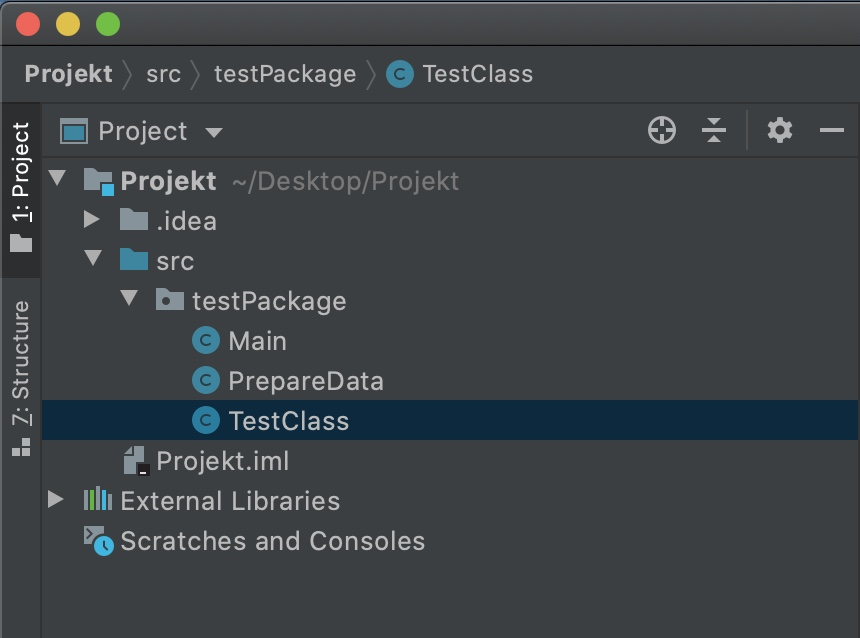
\includegraphics[width=\linewidth]{Images/img1.jpg}
  \caption{Darstellung eines Bahnhofs}
\end{figure}

\subsection{Tabelle}

\begin{table}[h]
\begin{center}
\begin{tabular}[h]{c|c|c}
ICE 1 & ICE 2 & ICE 3 \\ \hline
200 km/h & 250 km/h  & 300 km/h  \\
\end{tabular}
\caption{Sehr sehr schöne Tabelle}
\end{center}
\end{table}
\newpage
\section{Ablauf der Fahrzeugsteuerung} \label{hauptprogrammKapitel}
Damit die Fahrzeugsteuerung gestarten werden kann, muss die Datei \textit{fahrzeugsteuerung.php} ausgeführt werden. Obligatorisch für die Fahrzeugsteuerung ist die Abschnittsüberwachung (\textit{abschnittueberwachung.php}), welche vor dem Start der Fahrzeugsteuerung ausgeführt werden muss und auf deren Verwendung und Funktionsweise in Kapitel \ref{main_5} eingegangen wird. Der Aufbau dieses Kapitels orientiert sich an dem Ablauf der Fahrzeugsteuerung, welcher in Abbildung \ref{fig:hauptprogramm} schematisch dargestellt wird.
\begin{center}
\begin{figure}
\centering
\begin{tikzpicture}[node distance=0.7cm, auto,]
\node[punkt] (a) {Einbindung aller benötigten Dateien};
\node[below=of a, punkt] (b) {Einlesen von statischen und mehrfach verwendeter Daten aus der \textit{MySQL}-Datenbank in den Cache};
\node[below=of b, punkt](c) {Ermittlung aller Fahrzeuge im eingleisigen Netz und den zugehörigen Daten};
\node[below=of c, punkt](d) {Berechnung der Fahrtverläufe aller Fahrzeuge};
\node[right=of d, punkt](e) {Übermittlung der \Gls{echtzeitdaten} an die Fahrzeuge};
\node[right=of e, punkt](f) {Überprüfung nach neuen Fahrzeugen, Fahrplanänderungen, Fahrstraßenänderungen und Positionskalibrierung};
\node[above=of f, punkt](g) {Neuberechnung der Fahrtverläufe (falls notwendig)};
\draw [pil] (a) -- (b);
\draw [pil] (b) -- (c);
\draw [pil] (c) -- (d);
\draw [pil] (d) -- (e);
\draw [pil] (e) -- (f);
\draw [pil] (f) -- (g);
\draw [pil] (g.west) -- +(-0.5,0) -| (e.north);
\end{tikzpicture}
\caption{Ablauf der Fahrzeugsteuerung}
\label{fig:hauptprogramm}
\end{figure}
\end{center}
\subsection{Einlesen von statischen und mehrfach verwendeten Daten aus der \textit{MySQL}-Datenbank in den Cache} \label{main_1}
Die Fahrzeugsteuerung benötigt als Grundlage für viele Berechnungen Daten aus der \textit{MySQL}-Daten\-bank. Damit diese Daten nicht bei jeder Verwendung erneut aus der Datenbank geladen werden müssen und somit die Anzahl an Datenbank-Abfragen möglichst gering gehalten werden kann, werden die wichtigsten Daten beim Programmstart bzw. bei der ersten Verwendung in den Cache geladen (Code-Beispiel \ref{lst:cacheVars}). Beispielhaft zu nennen sind hierbei \textit{\$cache\-Infra\-Laenge} (Länge aller \acp{infra} in Metern), \textit{\$cache\-Haltepunkte} (zugehörige \ac{infra}e für alle Betriebsstellen und Richtung), \textit{\$cacheZwischenhaltepunkte} (zugehörige \acp{infra} für alle Zwischen-Betriebsstellen, die nur einem \ac{infra} zugeordnet sind), \textit{\$cache\-Gbt\-To\-Infra} (Zuordnung der \acp{infra} zu den GBT-Abschnitten) und \textit{\$cache\-Infra\-To\-Gbt} (Zuordnung der GBT-Abschnitte zu  den \acp{infra}n).
\begin{lstlisting}[caption={Initialisierung der Cache Variablen \textit{(fahrzeug\-steu\-e\-rung.php)}},captionpos=b,label={lst:cacheVars}]
// Statische Daten einlesen
$cacheInfranachbarn = createCacheInfranachbarn();
$cacheInfradaten = createCacheInfradaten();
$cacheSignaldaten = createCacheSignaldaten();
$cacheInfraLaenge = createcacheInfraLaenge();
$cacheHaltepunkte = createCacheHaltepunkte();
$cacheZwischenhaltepunkte = createChacheZwischenhaltepunkte();
$cacheInfraToGbt = createCacheInfraToGbt();
$cacheGbtToInfra = createCacheGbtToInfra();
$cacheFmaToInfra = createCacheFmaToInfra();
$cacheInfraToFma = array_flip($cacheFmaToInfra);
$cacheFahrplanSession = createCacheFahrplanSession();
$cacheSignalIDToBetriebsstelle = createCacheToBetriebsstelle();
$cacheFahrzeugeAbschnitte = createCacheFahrzeugeAbschnitte();
$cacheIDTDecoder = createCacheDecoderToAdresse();
$cacheDecoderToID = array_flip($cacheIDTDecoder);
$cacheAdresseToID = array();		// Filled with data in getAllTrains()
$cacheIDToAdresse = array();		// Filled with data in getAllTrains()
\end{lstlisting}
\subsection{Ermittlung der Session-Daten} \label{main_12}
In der \textit{MySQL}-Tabelle \textit{fahrplan\_session} sind alle Fahrplansessions aufgelistet und der aktuell gültigen wurde der Wert 1 in der \textit{status}-Spalte zugeordnet. Die Daten der gültigen Fahrplansession wurden bei dem Start der Fahrzeugsteuerung in dem Array \textit{\$cacheFahrplanSession} gespeichert und werden benötigt, um die Zeitdifferenz zwischen Real- und \Gls{simulationszeit} zu ermitteln. Dafür wird im ersten Schritt das Datum der \textit{sim\_startzeit} und \textit{sim\_endzeit}, welche die Start- und Endzeit (\Gls{simulationszeit}) der Simulation im \Gls{unix}-Format angeben, auf das aktuelle Datum der \Gls{realzeit} geändert und im zweiten Schritt mit der \Gls{realzeit} verglichen (Code-Beispiel \ref{lst:readTime}).

Das Datum der \Gls{simulationszeit} wird angepasst, damit auch Fahrplansessions ausgeführt werden können, die nicht dem aktuellen Datum der \Gls{realzeit} entsprechen. Für die Umwandlung des Datums werden die Zeiten mittels der Funktion \textit{getUhrzeit$($$)$}$^\ast$ in das \textit{hh:mm:ss}-Format umgewandelt und mit derselben Funktion wieder in das \Gls{unix}-Format zurück umgewandelt.

Für die Ermittlung der \Gls{realzeit} und der Zeitdifferenz zwischen Real- und \Gls{simulationszeit} wird die Funktion \textit{time$($$)$} aufgerufen, mit der Start-\Gls{simulationszeit} verglichen und unter der Variable \textit{\$timeDifference} abgespeichert.

Die Differenz zwischen Real- und \Gls{simulationszeit} ist es­sen­zi­ell, damit die Fahrzeuge zur richtigen Zeit die \Gls{echtzeitdaten} übermittelt bekommen und die \Gls{realzeit} in die \Gls{simulationszeit} umgewandelt werden kann, ohne bei jeder Umrechnung die Funktion \textit{getUhrzeit$($$)$}$^\ast$ aufzurufen.
\begin{figure}
\begin{lstlisting}[caption={Ermittlung der Real- und Simulationszeit \textit{(fahrzeug\-steu\-e\-rung.php)}},captionpos=b,label={lst:readTime}]
// Real- und Simulationszeit ermitteln
$simulationStartTimeToday = getUhrzeit(getUhrzeit($cacheFahrplanSession->sim_startzeit, "simulationszeit", null, array("outputtyp"=>"h:i:s")), "simulationszeit", null, array("inputtyp"=>"h:i:s"));
$simulationEndTimeToday = getUhrzeit(getUhrzeit($cacheFahrplanSession->sim_endzeit, "simulationszeit", null, array("outputtyp"=>"h:i:s")), "simulationszeit", null, array("inputtyp"=>"h:i:s"));
$simulationDuration = $cacheFahrplanSession->sim_endzeit - $cacheFahrplanSession->sim_startzeit;
$realStartTime = time();
$realEndTime = $realStartTime + $simulationDuration;
$timeDifference = $simulationStartTimeToday - $realStartTime;
\end{lstlisting}
\end{figure}
\subsection{Ermittlung aller Fahrzeuge im eingleisigen Netz und den zugehörigen Daten} \label{main_2}
Das eingleisige Netz des \acp{ebuef} kann mittels der RailCom-Technik und den Decodern in den Fahrzeugen ermitteln, welches Fahrzeug aktuell welche \ac{infra}e belegt. Belegt ein Fahrzeug einen \ac{infra}, wird in der Tabelle \textit{fma} in der Spalte \textit{decoder\_adresse} die Adresse des Fahrzeugs hinterlegt und in der \textit{infra\_zustand}-Tabelle in der Spalte \textit{dir} der Wert 1 hinterlegt. Durch diese Informationen werden alle Fahrzeuge, die sich beim Start des Programms im eingleisigen Netz befinden, mit der Funktion \textit{find\-Trains\-On\-The\-Tracks$($$)$} (\textit{functions.php}) eingelesen und die zugehörige Adresse wird der Funktion \textit{prepare\-Train\-For\-Ride$($$)$} (\textit{functions.php}) übergeben. Für jedes Fahrzeug, welches dieser Funktion übergeben wird, wird in dem Array \textit{\$allUsedTrains} ein neuer Eintrag erstellt, für jedes Fahrzeug die exakte Position bestimmt und der Fahrplan geladen. Das Array \textit{\$all\-Used\-Trains} beinhaltet alle Fahrzeuge, die aktuell von der Fahrzeugsteuerung berücksichtigt werden und deren zugehörige Informationen, wobei der Index der ID des Fahrzeugs entspricht. 

Bei der Positionsbestimmung wird davon ausgegangen, dass die Fahrzeuge direkt vor dem zugehörigen Signal stehen, da ansonsten die Position nicht exakt ermittelt werden kann. Belegt ein Fahrzeug mehrere \acp{infra}, wird mittels der Fahrtrichtung der Züge der \ac{infra} ermittelt, in dem sich der Zugkopf befindet. Die aktuelle Position wird daraufhin mit dem \ac{infra} und der relativen Position (in Metern) innerhalb des Abschnitts angegeben. Es wird davon ausgegangen, dass das Fahrzeug sich direkt vor dem Signal befindet, wodurch die relative Position der \ac{infra}slänge entspricht.

Für die Überprüfung, ob ein Fahrzeug nach Fahrplan fährt, wird die Funktion \textit{get\-Fahrzeug\-ZugIds$($$)$}$^\ast$ (\textit{functions\_ebuef.php}) aufgerufen. Wenn einem Fahrzeug kein Fahrplan zugewiesen wurde (Rückgabewert der Funktion \textit{get\-Fahrzeug\-ZugIds$($$)$}$^\ast$ (\textit{func\-tions\_""ebuef\-.php}) ist ein leeres Array), wird in dem \textit{\$allUsedTrains}-Array dem Fahrzeug unter dem Eintrag \textit{operates\_on\_timetable} der Wert \textit{false} zugewiesen. In dem Fall, dass für das Fahrzeug ein Fahrplan hinterlegt ist (Rückgabewert der Funktion \textit{get\-Fahrzeug\-ZugIds$($$)$}$^\ast$ (\textit{functions\_ebuef.php}) ist ein Array mit allen \Gls{zugid}s), wird mittels der Funktion \textit{getNextBetriebsstellen$($$)$} (\textit{functions.php}) der Fahrplan für den ersten Eintrag des \Gls{zugid} Arrays aus der Datenbank geladen. Der Fahrplan wird in dem \textit{\$all\-Used\-Trains}-Array in dem \textit{next\_betriebsstellen\_data}-Array hinterlegt, welches für jede Betriebsstelle ein Array mit den benötigten Daten enthält. Die Indizierung dieser Einträge entspricht dabei den natürlichen Zahlen in aufsteigender Reihenfolge angefangen bei der 0 ($\mathbb{N}_0$). Hierbei werden alle Betriebsstellen hinzugefügt, bei denen ein fahrplanmäßiger Halt vorgesehen ist. Damit ein Fahrzeug nicht erst losfahren kann, wenn die \Gls{fahrstrasse} bis zur nächsten Betriebsstelle mit fahrplanmäßigem Halt gestellt ist, werden auch alle Betriebsstellen ohne fahrplanmäßigem Halt hinzugefügt, welche eindeutig einem \ac{infra} zugeordnet sind (\textit{\$cacheZwischenhaltepunkte}). Das hat den Vorteil, dass Fahrzeuge losfahren können, auch wenn die \Gls{fahrstrasse} noch nicht bis zum nächsten fahrplanmäßigen Halt gestellt ist, das aber nur machen, wenn sichergestellt werden kann, dass die Zwischen-Betriebsstelle auf der Strecke zum nächsten fahrplanmäßigen Halt liegt. In Tabelle \ref{table:betriebsstellen} ist für eine bessere Übersicht der Aufbau eines Betriebsstellen-Eintrags abgebildet.
\begin{table}
\begin{center}
\renewcommand{\arraystretch}{1.2}
\begin{tabular}{c|c}
Bezeichnung & Funktion \\ \hline
\textit{is\_on\_fahrstrasse} (Boolescher Wert)                  		&    \makecell{Befindet sich die Betriebsstelle\\auf der \Gls{fahrstrasse}}                  \\ \hline
\textit{betriebstelle} (String)                  		&    Name der Betriebsstelle                  \\ \hline
\textit{zeiten} (Array)                  		&    \makecell{Verspätung und Ankunfts- und\\Abfahrtszeiten (siehe Tabelle \ref{table:betriebsstellenzeiten})}                  \\ \hline
\textit{haltepunkte} (Array)                  		&    Alle zugehörigen \acp{infra}                 \\ \hline
\textit{fahrplanhalt} (Boolescher Wert)             	&    Ist diese Betriebsstelle ein Fahrplanhalt               \\ 
\end{tabular}
\renewcommand{\arraystretch}{1}
\caption{Aufbau eines Arrays in \textit{next\_betriebsstellen\_data}}
\label{table:betriebsstellen}
\end{center}
\end{table}
Für die Ermittlung der Ankunfts- und Abfahrtzeiten wird die Funktion \textit{get\-Fahr\-plan\-zei\-ten$($$)$}$^\ast$ (\textit{functions\_ebuef.php}) aufgerufen, welche als Parameter den Namen der Betriebsstelle und die \Gls{zugid} übergeben bekommt. Die zurückgegebenen Daten werden unter dem Eintrag \textit{zeiten} abgespeichert und um den Eintrag \textit{verspaetung} ergänzt. Zudem werden die Ankunfts- und Abfahrtszeiten in das \Gls{unix}-Format mittels der Funktion \textit{getUhrzeit$($$)$}$^\ast$ (\textit{functions\_ebuef.php}) umgewandelt. Der Aufbau des \textit{zeiten}-Arrays ist in der Tabelle \ref{table:betriebsstellenzeiten} dargestellt.
\begin{table}
\begin{center}
\renewcommand{\arraystretch}{1.2}
\begin{tabular}{c|c}
Bezeichnung & Funktion \\ \hline
\textit{ankunft\_soll} (String)                  		&    Ankunftszeit (hh:mm:ss)                  \\ \hline
\textit{abfahrt\_soll} (String)                  		&     Abfahrtszeit (hh:mm:ss)                 \\ \hline
\textit{ankunft\_soll\_timestamp} (Integer)             	&   Ankunftszeit (Unixtimestamp)              \\ \hline
\textit{abfahrt\_soll\_timestamp} (Integer)             	&    Abfahrtszeit (Unixtimestamp)             \\ \hline
\textit{fahrtrichtung} (Array)                  		&   \makecell{Fahrtrichtung (Eintrag aus der Tabelle\\\textit{fahrplan\_sessionfahrplan})}                  \\ \hline
\textit{ist\_durchfahrt} (Integer)             	&    \makecell{Fahrplanhalt (Eintrag aus der Tabelle\\\textit{fahrplan\_sessionfahrplan})}               \\ \hline
\textit{used\_haltepunkt} (Integer)             	&    \makecell{\ac{infra} der Betriebsstelle,\\welcher auf der \Gls{fahrstrasse} liegt}             \\ \hline
\textit{wendet} (Integer)             	&    \makecell{Wendeauftrag nach\\Erreichen der Betriebsstelle}                \\ \hline
\textit{verspaetung} (Integer)             	&    \makecell{Verspätung, mit der das Fahrzeug\\diese Betriebsstelle erreicht hat}               \\ 
\end{tabular}
\renewcommand{\arraystretch}{1}
\caption{Aufbau des \textit{zeiten}-Arrays in \textit{next\_""betriebs\-stellen\_""data}}
\label{table:betriebsstellenzeiten}
\end{center}
\end{table}
Für die Überprüfung, ob eine Betriebsstelle durch die aktuelle \Gls{fahrstrasse} erreichbar ist, müssen den Betriebsstellen die \ac{infra}e zugeordnet werden. Dafür werden mit Hilfe der Arrays \textit{\$cache\-Zwischen\-halte\-punkte} und \textit{\$cache\-Halte\-punkte}, jeder Betriebsstelle mögliche \ac{infra}e zugeordnet. Die Arrays sind so aufgebaut, dass jeder Betriebsstelle für jede Richtung alle \ac{infra}e zugeteilt sind, welchen ein Ausfahrsignal zugeordnet ist.

Nach der Zuordnung der \ac{infra}e zu den Betriebsstellen, wird anhand der aktuellen Positionen der Fahrzeuge überprüft, ob die Fahrzeuge an einer Betriebsstelle des Fahrplans stehen. Stimmt der aktuelle \ac{infra} eines Fahrzeugs mit dem einer Betriebsstelle überein, wird dieser und allen vorherigen der Wert \textit{true} unter der Variablen \textit{angekommen} zugewiesen. Dadurch können Fahrzeuge auch nach Fahrplan fahren, wenn diese nicht an der ersten Betriebsstelle des Fahrplans stehen. 
\subsection{Berechnung der Fahrtverläufe aller Fahrzeuge} \label{main_3}
Nachdem für alle Fahrzeuge die Fahrplandaten (falls vorhanden) hinterlegt wurden, wird für jedes Fahrzeug die aktuelle  \Gls{fahrstrasse} ermittelt. Dafür wird die Funktion \textit{calculateNextSections$($$)$} (\textit{functions.php}) aufgerufen und das Array \textit{\$allUsedTrains} für jedes Fahrzeug um die Einträge \textit{next\_sections}, \textit{next\_lenghts} und \textit{next\_""v\_""max} als Array ergänzt. Diese Arrays speichern die IDs, Längen und zulässigen Höchstgeschwindigkeiten der nächsten \acp{infra} ab, welche auf der \Gls{fahrstrasse} liegen. 

Im ersten Schritt wird überprüft, ob das Fahrzeug aktuell in einem \ac{infra} steht, welchem ein auf Halt stehendes Signal zugeordnet ist. Wenn das der Fall ist, wird den Arrays \textit{next\_sections}, \textit{next\_lenghts} und \textit{next\_v\_max} ein leeres Array zugewiesen. Wenn das Fahrzeug aktuell nicht in einem Abschnitt steht, welchem ein auf Halt stehendes Signal zugeordnet ist, wird über die Funktion \textit{getNaechsteAbschnitte$($$)$}$^\ast$ (\textit{functions\_ebuef.php}) die aktuelle \Gls{fahrstrasse} ermittelt und der Rückgabewert der Funktion \textit{getNaechsteAbschnitte$($$)$}$^\ast$ (\textit{functions\_ebuef.php}) in dem \textit{\$allUsedTrains}-Array unter dem Eintrag \textit{last\_get\_naechste\_abschnitte} gespeichert. Diese Speicherung ist notwendig, um zu überprüfen, ob sich die \Gls{fahrstrasse} geändert hat. 

Nach der Ermittlung der \Gls{fahrstrasse} und der Zuordnung der \acp{infra} zu den Betriebsstellen wird im nächsten Schritt überprüft, welche Betriebsstellen des Fahrplans auf der aktuellen \Gls{fahrstrasse} liegen. Dafür iteriert die Funktion \textit{check\-If\-Fahr\-strasse\-Is\-Corrrect$($$)$} (\textit{functions.php}) in aufsteigender Reihenfolge über alle Betriebsstellen der Fahrzeuge und die \textit{haltepunkte} der Betriebsstellen werden mit den Werten aus dem Array \textit{next\_sections} verglichen. Bei jedem Aufruf der Funktion wird dem Fahrzeug anfangs (falls das Fahrzeug nach Fahrplan fährt) in dem Array \textit{\$allUsedTrains} der Eintrag \textit{fahrstrasse\_is\_correct} der Wert \textit{false} zugewiesen und erst auf \textit{true} gesetzt, wenn eine Betriebsstelle auf der \Gls{fahrstrasse} liegt. Bei dem Iterieren über die Betriebsstellen wird jeder Betriebsstelle anfangs der Wert \textit{false} für den Eintrag \textit{is\_on\_fahrstrasse} zugeordnet und sobald ein \ac{infra} einer Betriebsstelle in dem Array \textit{next\_sections} ebenfalls vorhanden ist, wird dem Eintrag \textit{is\_on\_fahrstrasse} der Wert \textit{true} zugewiesen und unter dem Eintrag \textit{used\_haltepunkt} der \ac{infra} gespeichert, welcher auf der \Gls{fahrstrasse} liegt. Bei dem Iterieren über alle Betriebsstellen werden nur die Betriebsstellen beachtet, welche das Fahrzeug noch nicht erreicht hat (\textit{angekommen} == \textit{false}). Für Fahrzeuge ohne Fahrplan wird der Eintrag \textit{fahrstrasse\_is\_correct} direkt auf \textit{true} gesetzt.

Durch die Ermittlung der \Gls{fahrstrasse} kann für jedes Fahrzeug der Fahrtverlauf berechnet werden. Für die Berechnung der Fahrtverläufe wird für jedes Fahrzeug die Funktion \textit{calculateFahrtverlauf$($$)$} (\textit{functions.php}) aufgerufen und innerhalb der Funktion überprüft, ob die \Gls{fahrstrasse} richtig eingestellt ist (\textit{fahrstrasse\_is\_correct} == \textit{true}). Wenn die \Gls{fahrstrasse} richtig eingestellt ist, wird zwischen Fahrzeugen unterschieden, die nach Fahrplan fahren und Fahrzeugen, die keinen Fahrplan haben. 

Für Fahrzeuge mit Fahrplan muss im ersten Schritt die nächste Betriebsstelle ermittelt werden, an der das Fahrzeug anhalten muss. Dafür wird mit einer \textit{for}-Schleife über alle in \textit{next\_betriebsstellen\_data} hinterlegten Betriebsstellen iteriert, die das Fahrzeug noch nicht angefahren hat (\textit{angekommen} == \textit{false}), die auf der \Gls{fahrstrasse} liegen (\textit{is\_on\_fahrstrasse} == \textit{true}) und die ein fahrplanmäßiger Halt sind (\textit{fahrplanhalt} == \textit{true}). Sobald eine Betriebsstelle gefunden wurde, wird die \textit{for}-Schleife abgebrochen und der Index der Betriebsstelle als \textit{\$nextBetriebsstelleIndex} abgespeichert. Sollte unter den nächsten Betriebsstellen keine dabei sein, auf die diese Kriterien zutreffen, wird in einer zweiten \textit{for}-Schleife nach den selben Kriterien (außer dem des fahrplanmäßigen Halts) nach einer Betriebsstelle gesucht und sobald eine Betriebsstelle gefunden wurde, wird die Schleife abgebrochen und der Index der Betriebsstelle unter der Variablen \textit{\$nextBetriebsstelleIndex} abgespeichert. Sollte eine nächste Betriebsstelle für das Fahrzeug existieren wird in einer dritten \textit{for}-Schleife überprüft, ob zwischen der aktuellen Position und der nächsten Betriebsstelle eine Betriebsstelle ist, bei der das Fahrzeug einen Wendeauftrag bekommt. Sollte eine solche Betriebsstelle existieren, wird diese unter der Variablen \textit{\$nextBetriebsstelleIndex} abgespeichert. In dem Fall, dass keine nächste Betriebsstelle ermittelt werden konnte und das Fahrzeug aktuell eine Geschwindigkeit hat, für die gilt: $v>0$ $km/h$, wird eine Gefahrenbremsung eingeleitet (siehe Kapitel \ref{notbremsung}). 

Für alle Fahrzeuge, für die eine nächste Betriebsstelle ermittelt werden konnte, werden im Folgenden alle notwendigen Daten ermittelt. Dazu zählt, ob die Fahrzeuge nach dem Erreichen der Betriebsstelle einen Wendeauftrag erhalten sollen (\textit{wendet}-Eintrag der nächsten Betriebsstelle), in welchen \ac{infra} das Fahrzeug zum Stehen kommen soll (\textit{used\_haltepunkt}-Eintrag der nächsten Betriebsstelle) und an welcher relativen Position innerhalb des Abschnitts das Fahrzeug angehalten soll (Länge des \ac{infra}s). Neben den Informationen zur Position müssen die Informationen zur Zeit ermittelt werden. 

Für die Ermittlung der Ankunftszeit muss neben dem zugehörigen Eintrag \textit{ankunft\_soll\_timestamp} der Betriebsstelle die Verspätung berücksichtigt werden. Aus diesem Grund wird im ersten Schritt die zuletzt angefahren Betriebsstelle unter der Variablen \textit{\$prevBetriebsstelle} abgespeichert. Sollte die nächste Betriebsstelle der erste fahrplanmäßige Halt sein (Ankunftszeit nicht definiert), so wird als Start- und Zielzeit (\textit{\$startTime} und \textit{\$endTime}) die aktuelle \Gls{simulationszeit} verwendet. Wenn die nächste Betriebsstelle nicht dem ersten fahrplanmäßigen Halt entspricht, wird als Zielzeit die Ankunftszeit der Betriebsstelle festgelegt und als Startzeit die Abfahrtszeit der vorherigen Betriebsstelle (\textit{\$prevBetriebsstelle}) plus die eingetragene Verspätung der vorherigen Betriebsstelle. Sollte es zu dem Zeitpunkt der Berechnung keine vorherige Betriebsstelle geben (\textit{\$prevBetriebsstelle} == \textit{null}), so wird als Startzeit die aktuelle \Gls{simulationszeit} gewählt. Im zweiten Schritt wird überprüft, ob die Startzeit kleiner als die aktuelle \Gls{simulationszeit} ist und wenn das der Fall ist, wird die Startzeit gleich der \Gls{simulationszeit} gesetzt. Im dritten Schritt wird die Startzeit gleich der frühstmöglichen Startzeit des Fahrzeugs (\textit{earliest\_possible\_start\_time}-Eintrag des Fahrzeugs) gesetzt, falls die Startzeit kleiner ist. Der Eintrag \textit{earliest\_possible\_start\_time} der Züge gibt die frühstmögliche Abfahrtzeit der Züge an und wird zum Beispiel bei einem Wendeauftrag auf die aktuelle \Gls{simulationszeit} gesetzt und um 30 $s$ erhöht. 

Für alle Fahrzeuge, die ohne Fahrplan unterwegs sind, wird als Ziel-\ac{infra} der letzte \ac{infra} aus dem Array \textit{last\_get\_naechste\_abschnitte} verwendet, welchem ein Signal zugeordnet ist. Die Ziel-Position innerhalb des \ac{infra}s entspricht dabei ebenfalls der Länge des Abschnitts und die Überprüfung, ob ein Wendeauftrag nach dem Erreichen des Ziel-\ac{infra} dem Fahrzeug übermittelt werden soll, wird von dem Signalbegriff abgeleitet. Die Start- und Zielzeit entsprechen der aktuellen \Gls{simulationszeit}, bzw. der \textit{earliest\_possible\_start\_time}. Sollte keinem der nächsten \ac{infra}e aus dem \textit{last\_get\_naechste\_abschnitte}-Array ein Signal zugeordnet sein und die aktuelle Geschwindigkeit des Fahrzeugs ist größer als 0 $km/h$ sein, so wird eine Gefahrenbremsung eingeleitet. Andernfalls wird die Funktion an dieser Stelle abgebrochen und es wird wieder versucht einen \Gls{fahrtverlauf} zu berechnen, wenn sich die \Gls{fahrstrasse} geändert hat.

Nach der Ermittlung aller notwendigen Daten für die Berechnung des Fahrtverlaufs, wird für jedes Fahrzeug die Funktion \textit{updateNextSpeed$($$)$} (\textit{functions\_fahrtverlauf.php}) aufgerufen, welche den Fahrtverlauf berechnet und in Kapitel \ref{kapitelFahrtverlauf} im Detail beschrieben wird. Wichtig an dieser Stelle ist der Rückgabewert der Funktion, welcher für Fahrzeuge mit Fahrplan die Verspätung in Sekunden angibt, mit der das Fahrzeug die Ziel-Betriebsstelle erreicht, und wird unter dem Eintrag \textit{verspaetung} der zugehörigen Betriebsstelle gespeichert. Ob ein Fahrzeug eine Betriebsstelle mit einer Verspätung erreicht, kann nur ermittelt werden, wenn die Ankunftszeit definiert ist. Für den Fall, dass für ein Fahrzeug ein Fahrplan hinterlegt ist, das Fahrzeug in einem \ac{infra} steht, welchem keine Betriebsstelle des Fahrplans zugeordnet ist und die \Gls{fahrstrasse} so eingestellt ist, dass das Fahrzeug den ersten fahrplanmäßigen Halt anfahren könnte, kann nicht ermittelt werden, ob das Fahrzeug diese Betriebsstelle mit einer Verspätung erreicht, da für den ersten fahrplanmäßigen Halt in der \textit{MySQL}-Tabelle \textit{fahrplan\_sessionfahrplan} keine Ankunftszeit hinterlegt ist. Aus diesem Grund, wurde in der Datei \textit{global\_variables.php} die Variable \textit{\$globalFirstHaltMinTime} definiert, welche angibt, wie lange ein Fahrzeug an der ersten Betriebsstelle des Fahrplans halten soll. Wenn diese Zeit eingehalten werde kann, wird das Fahrzeug (sofern die \Gls{fahrstrasse} richtig eingestellt ist) zur Abfahrtszeit die Betriebsstelle verlassen. Andernfalls gilt für die Verspätung der ersten Betriebsstelle:
\begin{equation*}
\textrm{Verspätung} = \textrm{Ankunftszeit} + \textit{\$globalFirstHaltMinTime} - \textrm{Abfahrtszeit}
\end{equation*}
\subsection{Übermittlung der \Gls{echtzeitdaten} an die Fahrzeuge} \label{main_4}
Nach dem Aufruf der Funktion \textit{updateNextSpeed$($$)$} (\textit{functions\_fahrtverlauf.php}) sind für alle Fahrzeuge -- für die ein Fahrtverlauf berechnet wurde -- in dem Array \textit{\$allTimes} alle \Gls{echtzeitdaten} enthalten. Das Array beinhaltet für jedes Fahrzeug wiederum ein Array, welches unter der Adresse des Fahrzeugs abgespeichert ist, und beinhaltet alle \Gls{echtzeitdaten} eines Fahrzeugs. Der Aufbau eines Array mit \Gls{echtzeitdaten} ist in Tabelle \ref{table:aufbauAllTimes} dargestellt.
\begin{table}
\begin{center}
\renewcommand{\arraystretch}{1.4}
\begin{tabular}{c|c}
Bezeichnung & Funktion \\ \hline
\textit{live\_position} (Float)                  		&    absolute Position (kann weg...)                \\ \hline
\textit{live\_speed} (Integer)                  		&    Geschwindigkeit des Fahrzeugs                \\ \hline
\textit{live\_time} (Float)                  		&    Zeit der Übermittlung an das Fahrzeug                 \\ \hline
\makecell{\textit{live\_relative\_position}\\(Integer)}                  		&    relative Position im \ac{infra}                \\ \hline
\textit{live\_section} (Integer)                  		&    \ac{infra}                \\ \hline
\makecell{\textit{live\_is\_speed\_change}\\(Boolescher Wert)}                  		&    \makecell{Angabe, ob bei diesen \Gls{echtzeitdaten}\\die Geschwindigkeit verändert wird}                \\ \hline
\makecell{\textit{live\_target\_reached}\\(Boolescher Wert)}                  		&    Das Fahrzeug hat sein Ziel erreicht                \\ \hline
\textit{id} (String)                  		&    ID des Zugs                \\ \hline
\textit{wendet} (Boolescher Wert)                  		&    \makecell{Angabe, ob ein Wendeauftrag\\durchgeführt werden soll}                \\ \hline
\textit{betriebsstelle} (String)                  		&    Name der Betriebsstelle des nächsten Halts                \\ \hline
\makecell{\textit{live\_all\_targets\_reached}\\(Integer)}                  		&    Index der Betriebsstelle, die erreicht wurde                \\ 
\end{tabular}
\renewcommand{\arraystretch}{1}
\caption{Aufbau eines Eintrags aus dem\textit{\$allTimes}-Array}
\label{table:aufbauAllTimes}
\end{center}
\end{table}
In einer \textit{while}-Schleife wird über alle Einträge des \textit{\$allTimes}-Arrays iteriert und überprüft, ob der erste Eintrag eines Fahrzeugs \Gls{echtzeitdaten} enthält, welche an das Fahrzeug übermittelt werden müssen. Dafür wird der Eintrag \textit{live\_time} mit der aktuellen \Gls{simulationszeit} verglichen und die zugehörigen  \Gls{echtzeitdaten} an das Fahrzeug übermittelt, wenn der Eintrag \textit{live\_time} kleiner als die aktuelle \Gls{simulationszeit} ist. Nach jedem Durchlauf der \textit{while}-Schleife wird diese mit der Funktion \textit{sleep$($$)$} für 0,03 $s$ pausiert. An dieser Stelle wurde sich für einen Wert von 0,03 $s$ entschieden, da so die Position auf einen Meter genau bestimmt werden kann, wenn das Fahrzeug eine Geschwindigkeit von 120 $km/h$ hat.

Wenn für ein Fahrzeug neue \Gls{echtzeitdaten} vorliegen, wird im ersten Schritt überprüft, ob eine Geschwindigkeitsveränderung vorliegt (\textit{live\_is\_speed\_change} == \textit{true}) und die neue Geschwindigkeit (falls vorhanden) über die Funktion \textit{sendFahrzeugbefehl$($$)$}$^\ast$ (\textit{functions\_ebuef.php}) dem Fahrzeug übergeben und mittels einer Terminal-Ausgabe angezeigt. Im zweiten Schritt wird der aktuelle \ac{infra}, die aktuelle Position innerhalb des Abschnitts und die Geschwindigkeit in dem Array \textit{\$allUsedTrains} abgespeichert. 

Sollte das Fahrzeug nach dem Ausführen der \Gls{echtzeitdaten} einen Wendeauftrag bekommen und dementsprechend der Eintrag \textit{wendet} \textit{true} sein, so wird die Funktion \textit{change\-Direction$($$)$} (\textit{functions.php}) aufgerufen. In der Funktion wird neben der Fahrtrichtungsänderung die neue Position ermittelt (die Position eines Fahrzeugs wird durch den Zugkopf beschrieben) und überprüft, ob die Fahrtrichtung geändert werden kann. 
\begin{figure}
  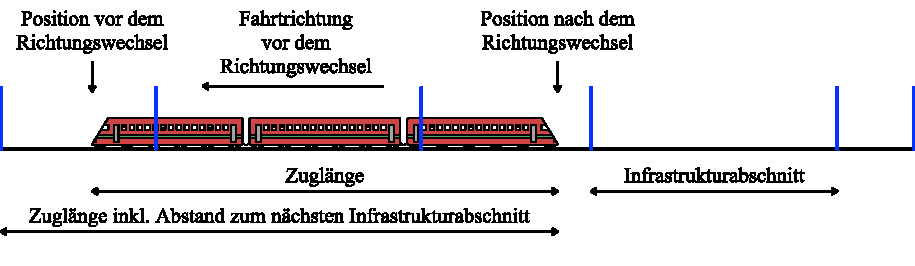
\includegraphics[width=\linewidth]{../images/vector/richtungsaenderung.pdf}
  \caption{Eigene Darstellung der Positionsbestimmung bei einem Richtungswechsel}
  \label{fig:richtungsaenderung}
\end{figure}
Damit die Fahrtrichtungsänderung ebenfalls funktioniert, wenn das Fahrzeug nicht am Ende eines \ac{infra}s steht, wird für die Ermittlung der neuen Position auf die Fahrzeuglänge der Abstand bis zum Ende \ac{infra}s addiert (siehe Abbildung \ref{fig:richtungsaenderung}). Über den aktuellen und die folgenden \acp{infra} (ermittelt durch die Funktion \textit{getNaechsteAbschnitte$($$)$}$^\ast$ (\textit{functions\_ebuef.php}), des aktuellen \ac{infra}s und der neuen Fahrtrichtung) wird iteriert und die Summe der Längen gebildet, bis die Fahrzeuglänge (zuzüglich des Abstands bis zum Ende des \ac{infra}s) überschritten wird. Der \ac{infra}, in dem die Fahrzeuglänge inkl. des Abstands zum ersten Mal überschritten wird, entspricht dem \ac{infra} der neuen Position.

Sollte die Länge aller nächsten Abschnitte inklusive des aktuellen Abschnitts in der Summe kleiner sein, als die Zuglänge inkl. dem Abstands bis zum Ende des Infra-Abschnitts, kann die neue Position nicht ermittelt werden und dem Fahrzeug wird eine Fehlermeldung übergeben, sodass das Fahrzeug nicht weiter fahren wird. Andernfalls wird die Richtung des Fahrzeugs in der Datenbank geändert und dem Fahrzeug mit der Funktion \textit{send\-Fahrzeugbefehl$($$)$}$^\ast$ (\textit{functions\_ebuef.php}) die Geschwindigkeit \mbox{-4 $km/h$} (entspricht einem Wendeauftrag) übergeben.

Bei einem \Gls{fahrtverlauf} kann es vorkommen, dass Fahrzeuge mit Fahrplan auf der Fahrt mehrere Betriebsstellen passieren. Damit dem Eintrag \textit{angekommen} dieser Betriebsstellen auch der Wert \textit{true} zugewiesen werden kann, wird überprüft, ob in den \Gls{echtzeitdaten} dem Eintrag \textit{live\_all\_targets\_reached} ein Wert zugewiesen ist. Dieser Eintrag enthält -- falls das Fahrzeug eine Betriebsstelle erreicht hat -- den Index der Betriebsstelle und weist der Betriebsstelle unter dem Eintrag \textit{angekommen} den Wert \textit{true} zu.

Wenn die letzten \Gls{echtzeitdaten} eines Fahrzeugs übermittelt wurden (\textit{live\_""target\_""reached} == \textit{true}) und das Fahrzeug dementsprechend zum Stehen gekommen ist, wird überprüft, wie sich das Fahrzeug als nächstes verhalten soll. Dafür wird zwischen vier Fällen (siehe Tabelle \ref{table:vierfaelle}) unterschieden.
\begin{table}
\begin{center}
\renewcommand{\arraystretch}{1.2}
\begin{tabular}{c|c|c}
 & Fährt jetzt ohne Fahrplan & Fährt jetzt nach Fahrplan \\ \hline
Fuhr davor ohne Fahrplan                 		&    1. Fall         & 2. Fall       \\ \hline
Fuhr davor nach Fahrplan                   		&    3. Fall         & 4. Fall       \\ 
\end{tabular}
\renewcommand{\arraystretch}{1}
\caption{Verhalten eines Fahrzeugs nach dem Erreichen des Ziels}
\label{table:vierfaelle}
\end{center}
\end{table}
Für die Überprüfung, ob sich der Fahrplan eines Fahrzeugs geändert hat, wird über die Funktion \textit{getFahrzeugZugIds$($$)$} (\textit{functions\_ebuef.php}) die aktuelle \Gls{zugid} abgefragt und mit der vorherigen verglichen. In dem \textbf{1. Fall} (alte und neue \Gls{zugid} haben beide den Wert \textit{null}) werden dem Fahrzeug keine neue Daten übergeben und ein neuer Fahrtverlauf wird versucht zu berechnen, sobald die \Gls{fahrstrasse} sich verändert hat. In dem \textbf{2.} und \textbf{4. Fall} wird die neue \Gls{zugid} dem Fahrzeug übergeben, der Eintrag \textit{operates\_on\_time\-table} auf \textit{true} gesetzt und die Funktionen \textit{get\-Fahr\-plan\-And\-Po\-sition\-For\-One\-Train$($$)$} (\textit{func\-tions.php}), \textit{add\-Stop\-sections\-For\-Time\-table$($$)$} (\textit{func\-tions.php}), \textit{calculate\-Next\-Sec\-tions$($$)$} (\textit{func\-tions\_fahrtverlauf.php}), \textit{check\-If\-Fahrstrasse\-Is\-Corrrect$($$)$} (\textit{func\-tions.php}) und \textit{calculate\-Fahrt\-ver\-lauf$($$)$} (\textit{func\-tions\-.php}) aufgerufen. Abgesehen von der ersten Funktion, werden diese Funktionen auch beim Start des Programms ausgeführt, welcher in Kapitel \ref{main_2} beschrieben wird. Die Funktion \textit{get\-Fahrplan\-And\-Position\-For\-One\-Train$($$)$} (\textit{func\-tions.php}) ähnelt der in Kapitel \ref{main_2} beschrieben Funktion \textit{pre\-pare\-Train\-For\-Ride$($$)$} (\textit{func\-tions.php}), fügt aber nur die Position und den Fahrplan hinzu, da alle anderen Daten schon eingelesen wurden. In dem \textbf{3. Fall} (die neu ermittelte \Gls{zugid} hat den Wert \textit{null}) wird der Eintrag \textit{operates\_on\_timetable} auf \textit{false} gesetzt und die Funktionen \textit{cal\-cu\-late\-Next\-Sec\-tions$($$)$} (\textit{func\-tions.php}) und \textit{cal\-cu\-late\-Fahrt\-ver\-lauf$($$)$} (\textit{func\-tions.php}) aufgerufen.
\subsection{Überprüfung nach einer Änderung der \Gls{fahrstrasse}}
Für die Überprüfung, ob sich die \Gls{fahrstrasse} der Züge verändert hat, wird in regelmäßigen Abständen die \Gls{fahrstrasse} der Fahrzeuge ermittelt und mit der aktuell hinterlegten \Gls{fahrstrasse} verglichen. Das Intervall, in dem diese Überprüfung stattfindet kann über die Variable \textit{\$timeCheckFahrstrasseInterval} (\textit{fahrzeugsteuerung.php}) festgelegt werden und ist standardgemäß auf 3 Sekunden festgelegt. Bei der Ermittlung und dem Vergleich der \Gls{fahrstrasse} wird für jedes Fahrzeug die Funktion \textit{compare\-Two\-Naechste\-Abschnitte$($$)$} (\textit{functions.php}) aufgerufen. Innerhalb dieser Funktion wird die in Kapitel \ref{main_2} erläutere Funktion \textit{calculateNextSections$($$)$} (\textit{functions.php}) aufgerufen, mit dem Unterschied, dass die ermittelten nächsten \acp{infra} inkl. der Längen und zulässigen Höchstgeschwindigkeiten nicht dem Fahrzeug hinterlegt werden, sondern lokal in der Funktion gespeichert. Damit die ermittelten Daten für ein Fahrzeug berechnet werden, aber nicht dem Fahrzeug hinterlegt werden, kann der Parameter \textit{\$writeResultToTrain} der Funktion \textit{calculateNextSections$($$)$} (\textit{functions.php}) (standardgemäß auf \textit{true} gesetzt) auf \textit{false} gesetzt werden. Sollte sich die \Gls{fahrstrasse} geändert haben, wird mit der Funktion \textit{check\-If\-Fahr\-strasse\-Is\-Corrrect$($$)$} (\textit{functions.php}) überprüft, ob die \Gls{fahrstrasse} dem Fahrplan (falls vorhanden) entspricht und im Anschluss die Funktion \textit{cal\-cu\-late\-Fahrt\-verlauf$($$)$} (\textit{functions.php}) aufgerufen.
\subsection{Neukalibrierung der Fahrzeugposition}  \label{main_5}
Für eine genau Fahrzeugsteuerung ist die aktuelle Position der Züge es­sen­zi­ell und muss während der Fahrt kalibriert werden, damit Ungenauigkeiten ausgeglichen werden können. Dafür werden die Daten aus der \textit{MySQL}-Tabelle \textit{fahrzeuge\_abschnitte} benötigt, welche durch die Abschnittsüberwachung ermittelt werden. Die Abschnittsüberwachung schreibt für jedes Fahrzeug den aktuellen \ac{infra} in die Datenbank, sobald der Zugkopf den Abschnitt befährt inklusive der aktuellen Zeit (\Gls{realzeit}). Für jedes Fahrzeug, welches durch die Übermittlung der \Gls{echtzeitdaten} in einen neuen \ac{infra} einfährt und seit der Einfahrt in den Abschnitt die Geschwindigkeit nicht verändert hat, wird die aktuelle Position neu ermittelt. Würde sich das Fahrzeug in einem \ac{infra} befinden und hätte seit der Einfahrt die Geschwindigkeit angepasst, könnte mit der Fahrzeugsteuerung die Position nicht neu berechnet werden, da nicht bekannt ist, welche Strecke das Fahrzeug seit der Einfahrt zurückgelegt hat. Aus diesem Grund wird, sobald das Fahrzeug nach den \Gls{echtzeitdaten} einen neuen Abschnitt befährt und aktuell nicht die Geschwindigkeit anpasst (\textit{live\_is\_speed\_change} == \textit{false}) dem Eintrag \textit{calibrate\_section\_one} der aktuelle \ac{infra} hinzugefügt und dem Eintrag \textit{calibrate\_section\_two} wird ebenfalls der aktuelle \ac{infra} hinzugefügt, wenn \textit{calibrate\_section\_one} ein Wert zugewiesen ist und dieser nicht dem aktuellen \ac{infra} der \Gls{echtzeitdaten} entspricht. Soabld das Fahrzeug seine Geschwindigkeit anpasst (\textit{live\_""is\_""speed\_""change} == \textit{true}), wird beiden Einträgen der Wert \textit{null} zugewiesen. Dadurch ist dem Eintrag \textit{calibrate\_section\_two} nur dann ein \ac{infra} zugewiesen, wenn das Fahrzeug in diesem seit der Einfahrt die Geschwindigkeit nicht verändert hat. Wenn dem Eintrag \textit{\$useRecalibration} aus der Datei \textit{global\_variables.php} der Wert \textit{true} zugewiesen ist, wird in regelmäßigen Abständen überprüft, ob eine Neukalibrierung möglich ist. Das Zeitintervall, in dem die Überprüfung stattfindet ist standardmäßig auf 3 Sekunden eingestellt, kann aber mittels der Variable \textit{\$timeCheckCalibrationInterval} (\textit{fahrzeugsteuerung.php}) angepasst werden.

Für die Neukalibrierung wird die Funktion \textit{getCalibratedPosition$($$)$} (\textit{functions.php}) (Code-Beispiel \ref{lst:getCalibratedPosition}) aufgerufen, welche als Rückgabewert die aktuelle relative Position und den aktuellen \ac{infra} zurückgibt.
\begin{figure}
\begin{lstlisting}[caption={\textit{getCalibratedPosition$($$)$} (\textit{functions\_db.php})},captionpos=b,label={lst:getCalibratedPosition}]
// Kalibriert die Position des Fahrzeugs neu anhand der Daten in der Tabelle
// 'fahrzeuge_abschnitte'
function getCalibratedPosition ($id, $speed) {
	global $cacheFahrzeugeAbschnitte;
	$DB = new DB_MySQL();
	$positionReturn = $DB->select("SELECT `".DB_TABLE_FAHRZEUGE_ABSCHNITTE."`.`infra_id`,`".DB_TABLE_FAHRZEUGE_ABSCHNITTE."`.`unixtimestamp` FROM `".DB_TABLE_FAHRZEUGE_ABSCHNITTE."` WHERE `".DB_TABLE_FAHRZEUGE_ABSCHNITTE."`.`fahrzeug_id` = $id")[0];
	unset($DB);
	if (in_array($id, array_keys($cacheFahrzeugeAbschnitte))) {
		if ($positionReturn->unixtimestamp == $cacheFahrzeugeAbschnitte[$id]["unixtimestamp"]) {
			return array("possible" => false);
		}
	}
	$timeDiff = time() - $positionReturn->unixtimestamp;
	$position = ($speed / 3.6) * $timeDiff;
	return array("section" => $positionReturn->infra_id, "position" => $position);
}
\end{lstlisting}
\end{figure}

Sollte die ermittelte Position innerhalb des \ac{infra}s größer als die Länge des \ac{infra}s sein, welche in dem Array \textit{\$cacheInfraLaenge} abgespeichert ist, wird die Neukalibrierung nicht durchgeführt. Der aktuelle \ac{infra} wird aus der Tabelle \textit{fahrzeuge\_abschnitte} der \textit{MySQL}-Datenbank geladen und durch die aktuelle Geschwindigkeit des Fahrzeugs und die Differenz der Zeit zwischen dem Einfahren in den \ac{infra} und der aktuellen Zeit wird die relative Position innerhalb des \ac{infra}s berechnet.
\begin{equation*}
\textrm{relative Position} = \textrm{Geschwindigkeit} \cdot \textrm{Zeitdifferenz (aktuelle Zeit} - \textrm{Zeit des Einfahrens)}
\end{equation*}
\subsection{Ermittlung von neuen Fahrzeugen im eingleisigen Netz} \label{main_6}
Die Fahrzeugsteuerung betrachtet neben den Fahrzeugen, welche sich schon zu Beginn des Programmstarts im eingleisigen Netz befinden auch alle Fahrzeuge, die nach dem Programmstart hinzugefügt werden. Für alle Fahrzeuge, die beim Start des Programms erkannt werden, wird in dem Array \textit{\$allTrainsOnTheTrack} die zugehörige Adresse gespeichert (\textit{find\-Trains\-On\-The\-Tracks$($$)$}) (\textit{functions.php}). Für die Überprüfung, ob Fahrzeuge entfernt wurden oder neu hinzugekommen sind, wird die Funktion \textit{up\-date\-All\-Trains\-On\-The\-Track$($$)$} (\textit{functions.php}) verwendet. Diese Funktion wird -- wie die Neukalibrierung in Kapitel \ref{main_5} -- alle 3 Sekunden ausgeführt. Bei dem Aufruf der Funktion werden alle Fahrzeuge geladen, denen in der \textit{fma}-Tabelle aus der Datenbank ein \ac{infra} zugeordnet ist und mit dem Array \textit{\$allTrainsOnTheTrack} verglichen. Fahrzeugadressen, die nicht in dem Array hinterlegt sind, werden in dem Rückgabe-Array unter dem Eintrag \textit{new} zurückgegeben und alle Fahrzeugadressen, die in dem Array enthalten sind, aber bei dem Aufruf der Funktion keinem \ac{infra} zugeordnet sind, werden in dem Rückgabe-Array unter dem Eintrag \textit{removed} zurückgegeben. Nach dem Aufruf der Funktion, werden für alle neuen Fahrzeuge die Funktion \textit{pre\-pare\-Train\-For\-Ride$($$)$} (\textit{func\-tions.php}), \textit{add\-Stop\-sec\-tions\-For\-Time\-table$($$)$} (\textit{func\-tions.php}), \textit{cal\-culate\-Next\-Sec\-tions$($$)$} (\textit{func\-tions.php}), \textit{check\-If\-Train\-Reached\-Halte\-punkt$($$)$} (\textit{func\-tions.php}), \textit{check\-If\-Fahr\-strasse\-Is\-Corrrect$($$)$} (\textit{func\-tions.php}) und \textit{calculate\-Fahrt\-ver\-lauf$($$)$} (\textit{func\-tions\-.php}) aufgerufen (siehe Kapitel \ref{main_2} und \ref{main_3}). Alle entfernten Fahrzeuge werden aus dem Array \textit{\$allUsedTrains} entfernt und somit nicht mehr von der Fahrzeugsteuerung beachtet. 
\subsection{Fehlerbehebung von Fahrzeugen} \label{main_7}
Wenn es bei einem Fahrzeug zu einem Konflikt kommt, der eine Steuerung des Fahrzeugs verhindert, wird dem Fahrzeug eine Fehlermeldungs-ID unter dem Eintrag \textit{error} in dem \textit{\$allUsedTrains} zugewiesen. Fahrzeuge, denen eine Fehlermeldung zugeordnet wurde, werden ab diesem Zeitpunkt nicht weiter von der Fahrzeugsteuerung berücksichtigt. Für das Erkennen von Fahrzeugen mit Fehlermeldungen, wird in regelmäßigen Zeitintervallen (\textit{\$time\-Check\-All\-Train\-Sta\-tus\-Inter\-val}) die Funktion \textit{showErrors$($$)$} (\textit{functions.php}) aufgerufen, welche die Fehlermeldungen aller Fahrzeuge ausgibt (Code-Beispiel \ref{lst:showErrors}).
\begin{figure}
\begin{lstlisting}[caption={\textit{showErrors$($$)$} (\textit{functions.php})},captionpos=b,label={lst:showErrors}]
// Gibt für alle Fahrzeuge die vorhanden Fehlermeldungen an.
function showErrors() {

	global $allUsedTrains;
	global $trainErrors;

	$foundError = false;
	echo "Hier werden für alle Züge mögliche Fehler angezeigt:\n\n";

	foreach ($allUsedTrains as $trainIndex => $trainValue) {
		if (sizeof($trainValue["error"]) != 0) {
			$foundError = true;
			echo "Zug ID: ", $trainValue["id"], "\n";
			$index = 1;

			foreach ($trainValue["error"] as $error) {
				echo "\t", $index, ". Fehler:\t", $trainErrors[$error], "\n";
				$index++;
			}

			echo "\n";
		}
	}

	if (!$foundError) {
		echo "Keiner der Züge hat eine Fehlermeldung.\n";
	}
}
\end{lstlisting}
\end{figure}
Für das Beheben einer Fehlermeldung muss das Fahrzeug händisch vom Schienennetz genommen werden, gewartet werden, bis die Fahrzeugsteuerung das Entfernen registriert hat und das Fahrzeug wieder händisch auf das Schienennetz gesetzt werden.

Die möglichen Fehlermeldungen sind in dem Array \textit{\$trainErrors} gespeichert und können um beliebig viele weitere Fehlermeldungen ergänzt werden. Für die Implementierung einer neuen Fehlermeldung muss lediglich die Fehlermeldungs-ID (Index der Fehlermeldung in dem \textit{\$trainErrors}-Array) dem Eintrag \textit{error} aus dem \textit{\$allUsedTrains}-Array hinzugefügt werden, sobald der Konflikt in der Fahrzeugsteuerung auftritt.
\begin{table}
\begin{center}
\renewcommand{\arraystretch}{1.2}
\begin{tabular}{c|c}
Fehlermeldungs-ID & Beschreibung  \\ \hline
0 &    \makecell{Fahrtrichtung des Fahrzeugs musste geändert werden\\und die Positionsbestimmung war nicht möglich} \\\hline
1              &    \makecell{In der Datenbank ist für das Fahrzeug\\keine Zuglänge angegeben}             \\ \hline
2         &    \makecell{In der Datenbank ist für das Fahrzeug\\keine v\_max angegeben}             \\ \hline
3        &   \makecell{Das Fahrzeug musste eine\\Gefahrenbremsung durchführen}          \\ 
\end{tabular}
\renewcommand{\arraystretch}{1}
\caption{Übersicht der Fehlermeldungen}
\label{table:fehlertabelle}
\end{center}
\end{table}
In Tabelle \ref{table:fehlertabelle} sind alle Fehlermeldungen aufgelistet, welche aktuell in der Fahhrzeugsteuerung implementiert sind.
%\linebreak[4] -> behält blocksatz bei








































\newpage
\section{Berechnung des \Gls{fahrtverlauf}s} \label{kapitelFahrtverlauf}
Der \Gls{fahrtverlauf} eines Fahrzeuges wird bei der Berechnung auf zwei verschiedenen Arten gespeichert. Einmal in so genannten \textit{\$keyPoints}, welche in einem Array die Start- und Zielgeschwindigkeit (\textit{speed\_0} und \textit{speed\_1}), die Start- und Endposition (\textit{position\_0} und \textit{position\_1}) und die Start- und Endzeit (\textit{time\_0} und \textit{time\_1}) der einzelnen Beschleunigungen bzw. Verzögerungen abspeichern. Für die Überprüfung, ob ein Fahrzeug die zulässige Höchstgeschwindigkeit in einem \ac{infra} überschreitet, für die spätere Übermittlung der \Gls{echtzeitdaten} an das Fahrzeug und die exakte Positionsbestimmung, werden mittels der \textit{\$keyPoints} für jede Geschwindigkeitsänderungen (und bei \Gls{beharrungsfahrt}en in 1 Meter Abständen) unter anderem die aktuelle relative Position innerhalb eines \ac{infra}s (\textit{\$trainRelativePosition}), der \ac{infra} (\textit{\$trainSection}), die aktuelle Zeit (\textit{\$trainTimeChange}) und die aktuelle Geschwindigkeit (\textit{\$trainSpeedChange}) in gespeichert. 

Als Grundlage für die Berechnung des \Gls{fahrtverlauf}s werden zudem die Variablen \textit{\$indexCurrentSection} und \textit{\$indexTargetSection} benötigt, welche die Indexe der Start- und Ziel-\ac{infra}e in Bezug auf das Array \textit{\$next\_sections} beschreiben und die Arrays \textit{\$cumulativeSectionLengthStart} und \textit{\$cumulativeSectionLengthEnd}, welche für jeden \ac{infra} den Abstand zur aktuellen Position von dem Anfang und dem Ende des \ac{infra}s angeben.

Der \Gls{fahrtverlauf} wird mit der Funktion \textit{updateNextSpeed$($$)$} (\textit{functions\_fahrt\-ver\-lauf.php}) berechnet, welche als Parameter unter anderem die Zugdaten aus dem \textit{\$all\-Used\-Trains}-Array, Start- und Endzeit der Fahrt (\textit{\$startTime} und \textit{\$endTime}), den Ziel-\ac{infra} (\textit{\$targetSection}) und die relative Position in dem Ziel-\ac{infra} (\textit{\$targetPosition}) übergeben bekommt.
\begin{table}
\begin{center}
\renewcommand{\arraystretch}{1.2}
\begin{tabular}{c|c}
Bezeichnung & Funktion \\ \hline
\textit{\$keyPoint} (Array)                   			&   \makecell{Beschreibt eine Beschleunigung bzw.\\Verzögerung (\textit{position\_0}, \textit{position\_1},\\ \textit{time\_0}, \textit{time\_1}, \textit{speed\_0}, \textit{speed\_1})}           \\ \hline
\textit{\$next\_section} (Array)                  		&    IDs aller \ac{infra}e                  \\ \hline
\textit{\$next\_lenghts} (Array)                  		&    Längen aller \ac{infra}e                  \\ \hline
\textit{\$next\_v\_max} (Array)                  		&    Höchstgeschwindigkeit aller \ac{infra}e                  \\ \hline
\textit{\$indexCurrentSection} (Integer)             	&    Index des aktuellen \ac{infra}s               \\ \hline
\textit{\$indexTargetSection} (Integer)               	&    Index des Ziel-\ac{infra}s                  \\ \hline
\makecell{\textit{\$cumulativeSectionLengthStart}\\(Array) }	&    Absolute Startposition aller \ac{infra}e                  \\ \hline
\makecell{\textit{\$cumulativeSectionLengthEnd}\\(Array)  }	&    Absolute Endposition aller \ac{infra}e                  \\ \hline
\textit{\$trainPositionChange} (Array)                	&    Alle absoluten Positionen des \Gls{fahrtverlauf}s                  \\ \hline
\textit{\$trainSpeedChange} (Array)                  	&   Alle Geschwindigkeiten des \Gls{fahrtverlauf}s                  \\
\end{tabular}
\renewcommand{\arraystretch}{1}
\caption{Beschreibung der verwendeten Variablen für die \Gls{fahrtverlauf}sberechnung}
\label{table:vars}
\end{center}
\end{table}

In dem folgenden Abschnitt werden die einzelnen Schritte beschrieben, die durchlaufen werden, um den optimalen \Gls{fahrtverlauf} zu berechnen. In der Darstellung \ref{fig:fahrtverlauf} wird der Ablauf grob schematisch dargestellt.
\begin{figure}
\resizebox{1\textwidth}{!}{
\begin{tikzpicture}[node distance=1cm, auto]
\node[punkt] (a) {Berechnung bei einer Beschleunigung auf die maximal mögliche Geschwindigkeit};
\node[below=of a, punkt] (b) {Wird die Geschwindigkeit in \ac{infra}n überschritten?};
\node[right=of b, punkt](c) {Neuberechnung unter Berücksichtigung der Geschwindigkeitsüberschreitung};
\node[below=of b, punkt] (d) {Wird die Mindestzeit auf den \Gls{beharrungsfahrt}en eingehalten?};
\node[right=of d, punkt](e) {Neuberechnung unter Berücksichtigung der Mindestzeit auf einer Geschwindigkeit};
\node[below=of d, punkt] (f) {Erreicht der Fahrzeug mit einer Verspätung das Ziel?};
\node[right=of f, punkt] (g) {Kann die Geschwindigkeit reduziert werden, ohne dass das Fahrzeug eine Verspätung hat?};
\node[below=of f, punkt] (h) {Übermittlung der \Gls{echtzeitdaten} an das Fahrzeug};
\node[right=of g, punkt] (i) {Reduzierung der Geschwindigkeit unter Einhaltung der Ankunftszeit};
\node[right=of a, punkt] (j) {Ist eine Fahrt ohne Gefahrenbremsung möglich?};
\node[right=of j, punkt] (k) {Berechnung der Gefahrenbremsung};
\node[above=of j, punkt] (l) {Start der \Gls{fahrtverlauf}sberechnung};
\draw [pil] (a) -- (b);
\draw [pil] (b) --  node[pos=0.5] {Ja} (c);
\draw [pil] (c.north) -- +(0,0.4) -|  (b.north); 
\draw [pil] (b) -- node[pos=0.5,left] {Nein} (d);
\draw [pil] (d) --  node[pos=0.5] {Nein} (e);
\draw [pil] (e.north) -- +(0,0.3) -|  (d.north); 
\draw [pil] (d) -- node[pos=0.5,left] {Ja} (f);
\draw [pil] (f) -- node[pos=0.5] {Ja} (g);
\draw [pil] (f) -- node[pos=0.5,left] {Nein} (h);
\draw [pil] (g) -- node[pos=0.5] {Ja} (i);
\draw [pil] (g.south) -- node[pos=0.5,left] {Nein} +(0,-1) |-  (h.east); 
\draw [pil] (i.south) -- +(0,-1) |-  (h.east); 
\draw [pil] (j) -- node[pos=0.5,above] {Ja} (a);
\draw [pil] (j) -- node[pos=0.5] {Nein} (k);
\draw [pil] (l) -- (j);
\draw [pil] (k.east) -- +(0.5,0) |- (h.east);
\end{tikzpicture}
}
\caption{Ablaufplan der \Gls{fahrtverlauf}sberechnung}
\label{fig:fahrtverlauf}
\end{figure}
\subsection{Ermittlung der Start- und Endposition der einzelnen \ac{infra}e unter Berücksichtigung der Zuglänge}
Für die Berechnung eines exemplarischen \Gls{fahrtverlauf}s wurden die in Tabelle \ref{table:infraex} definierten \ac{infra}e verwendet. Diese \ac{infra}e wurden so gewählt, dass alle Funktionen und die Allgemeingültigkeit des Algorithmus gezeigt werden können und existieren in dieser Form im \ac{ebuef} nicht. 
\begin{table}
\begin{center}
\renewcommand{\arraystretch}{1.2}
\begin{tabular}{c| C{2cm} |c}
\ac{infra}s-ID & Länge & zulässige Höchstgeschwindigkeit \\ \hline
1000                   &   300 $m$    & 120 $km/h$                        \\ \hline
1001                  &    400 $m$   & 120 $km/h$                        \\ \hline
1002                   &   300 $m$    &        120 $km/h$                         \\ \hline
1003                   &    400 $m$   &         90 $km/h$                        \\ \hline
1004                   &    300 $m$   &            60 $km/h$                     \\ \hline
1005                   &   200 $m$    &           60 $km/h$                      \\ \hline
1006                   &  400 $m$     &      90 $km/h$                           \\ \hline
1007                   &  500 $m$     &      120 $km/h$                           \\ \hline
1008                   &   300 $m$    &      120 $km/h$                           \\ \hline
1009                   &   400 $m$    &      100 $km/h$                           \\ \hline
1010                   &   300 $m$    &      60 $km/h$                           \\ \hline
1011                   &   300 $m$    &         40 $km/h$                        \\ 
\end{tabular}
\renewcommand{\arraystretch}{1}
\caption{Exemplarische \ac{infra}e}
\label{table:infraex}
\end{center}
\end{table}
Als exemplarisch gewählte Zugdaten wurden die in Tabelle \ref{table:train-ex} definierten Daten verwendet.
\begin{table}[]
\begin{center}
\renewcommand{\arraystretch}{1.2}
\begin{tabular}{r L{3cm}}
relative Startposition                   &   10 $m$                         \\ 
relative Zielposition                  &    290 $m$                         \\ 
aktueller \ac{infra}                   &   1001                         \\ 
Ziel-\ac{infra}                  &    1010                         \\ 
Startgeschwindigkeit                   &   0 $km/h$                          \\ 
Zielgeschwindigkeit                   &    0 $km/h$                        \\ 
Zuglänge                   &    50 $m$                        \\ 
Bremsverzögerung                   &    0,8 $m/s^{2}$                        \\ 
Fahrplan vorhanden                   &    ja                        \\ 
Zeit bis zur nächsten Betriebsstelle                   &    210 $s$                        \\ 
\end{tabular}
\renewcommand{\arraystretch}{1}
\caption{Exemplarische Zugdaten}
\label{table:train-ex}
\end{center}
\end{table}

Die zuvor ermittelten nächsten \ac{infra}e inklusive derer Längen und zulässigen Höchstgeschwindigkeit müssen für die Berechnung des \Gls{fahrtverlauf}s angepasst werden, da ein Fahrzeug erst beschleunigen darf, wenn das komplette Fahrzeug in den \ac{infra} eingefahren ist. In Darstellung \ref{fig:it1} sind die \ac{infra}e dargestellt, wie sie von der Fahrzeugsteuerung ermittelt wurden. Dabei werden alle \ac{infra}e, die das Fahrzeug bereits durchfahren hat oder hinter dem Ziel-\ac{infra} liegen nicht dargestellt. Zudem wird in dem aktuellen \ac{infra} die relative Position von der Länge abgezogen und der Ziel-\ac{infra} wird nur bis zur relativen Zielposition abgebildet. Dementsprechend ist der erste \ac{infra} in der Darstellung \ref{fig:it1} der \ac{infra} mit der ID 1001. Dieser hat aufgrund der aktuellen relativen Position des Fahrzeugs eine Länge von 290 $m$. Und der letzte \ac{infra} ist der \ac{infra} mit der ID 1010 und einer Länge von ebenfalls 290 $m$.
\begin{figure}
  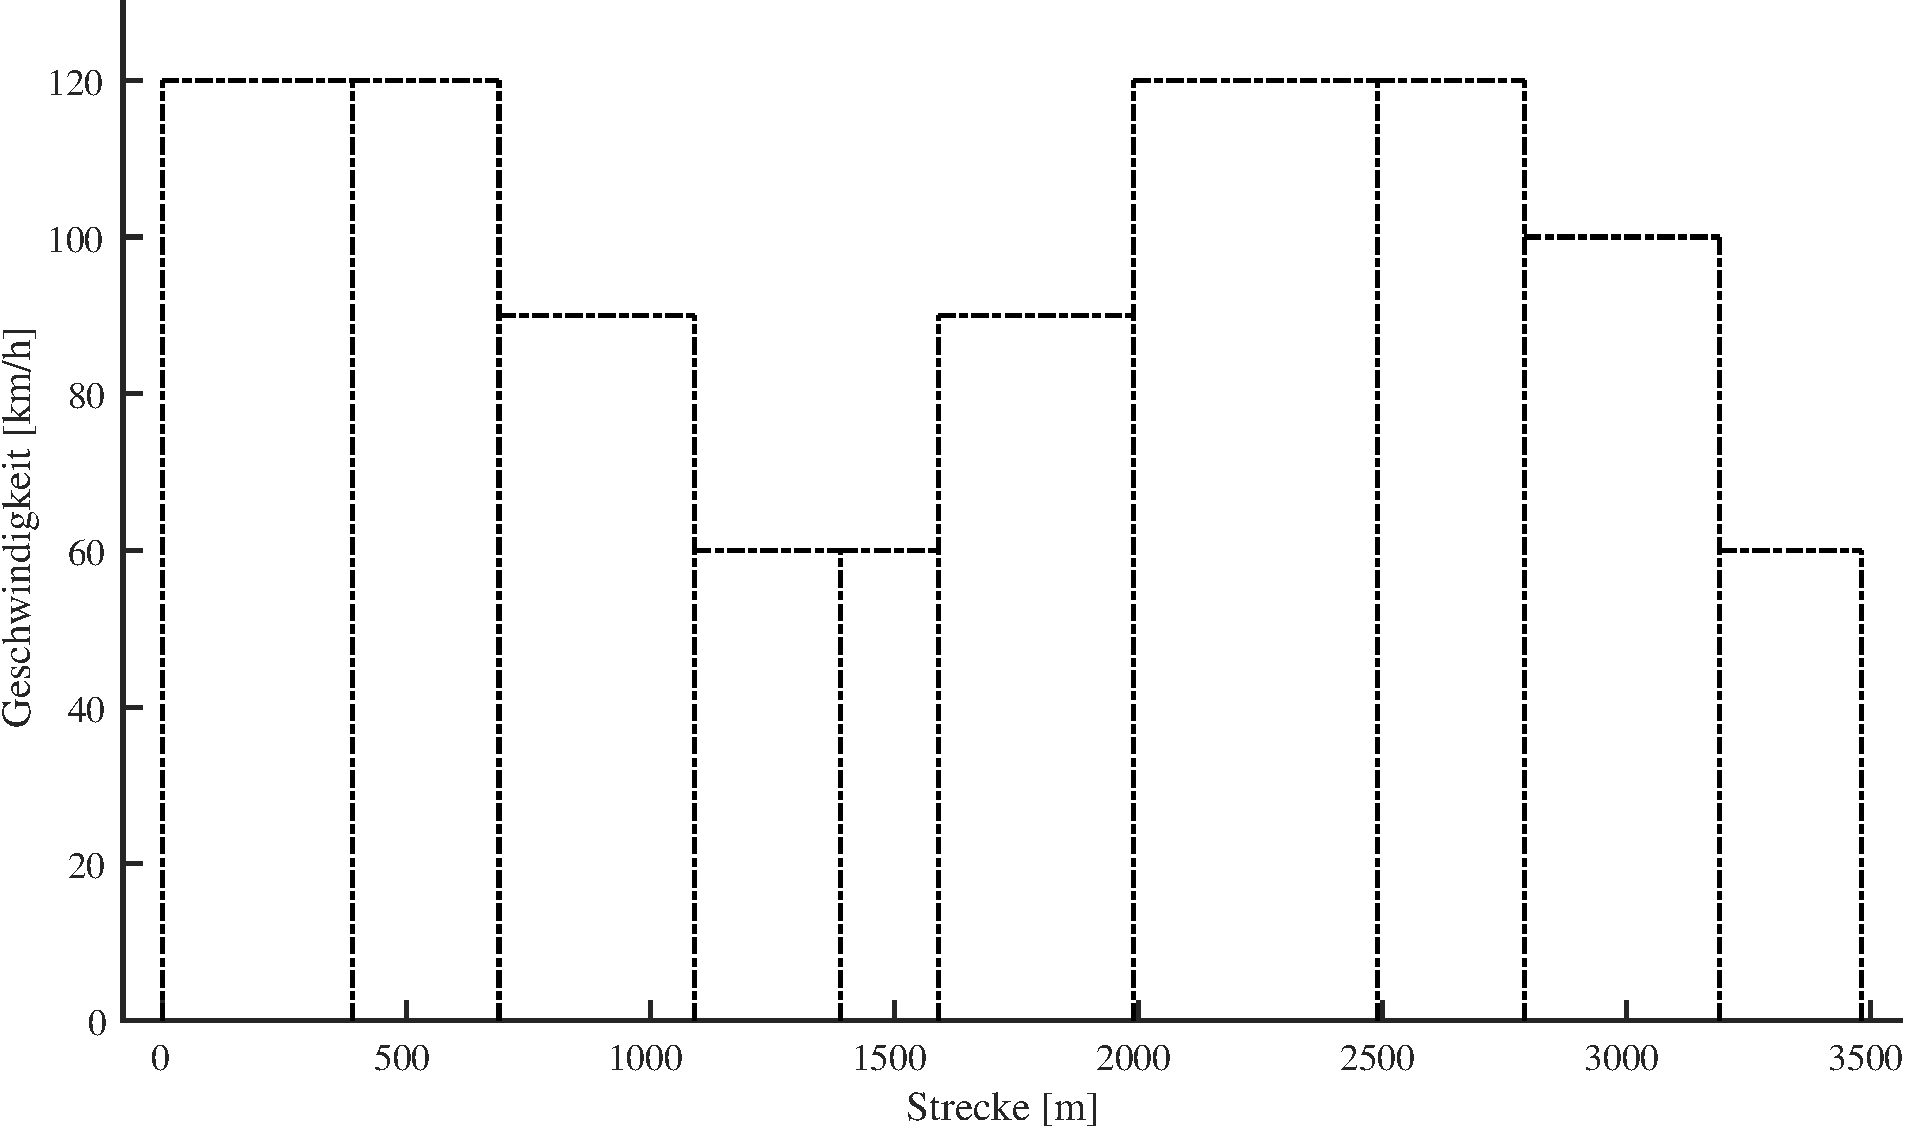
\includegraphics[width=\linewidth]{../images/matlab/it1.pdf}
  \caption{Infra-Abschnitte und die zugehörige Höchstgeschwindigkeit}
  \label{fig:it1}
\end{figure}

Bei der Berücksichtigung der Fahrzeuglänge wird mit einer \textit{for}-Schleife über alle \ac{infra}e iteriert und die Zuglänge auf die Länge das \ac{infra}s addiert. Von dieser neu ermittelten Endposition des \ac{infra}s wird überprüft, ob zwischen der vorherigen Endposition und der neu ermittelten Endposition ein \ac{infra} liegt, dessen zulässige Höchstgeschwindigkeit geringer ist, als die des ursprünglichen \ac{infra}s. Wenn dieser Fall eintritt, wird der \ac{infra} nur so weit verlängert, dass keine Höchstgeschwindigkeit der folgenden \ac{infra}e überschritten wird. Nach der Ermittlung der neuen Endposition, startet die \textit{for}-Schleife mit dem \ac{infra}, in dem sich die Endposition sich befindet. Sobald der Ziel-\ac{infra} erreicht wurde, wird die Schleife abgebrochen. Die neu ermittelten \ac{infra}e werden in den Arrays \textit{\$next\_lengths\_mod} und \textit{\$next\_v\_max\_mod} abgespeichert (analog zu den Arrays \textit{\$next\_lengths} und \textit{\$next\_v\_max}). 

Durch diesen Algorithmus kann es dazu kommen, dass sich die Anzahl der \ac{infra}e verändert hat, wodurch die \ac{infra}e nicht mehr eindeutig mit der Infrastruktur-ID bezeichnet werden können. Mittels \textit{\$next\_""lengths\_""mod} und \textit{\$next\_""v\_""max\_""mod} werden mit der Funktion \textit{create\-Cumulative\-Sec\-tions$($$)$} (\textit{func\-tions\_""fahrt\-ver\-lauf.php}) für jeden \ac{infra} die absolute Start- und Endposition in den Arrays \textit{\$cumulative\-Section\-Length\-Start\-Mod} und \textit{\$cumulativeSectionLengthEndMod} gespeichert. Diese Umwandlung ist essentiell für die Überprüfung, in welchem \ac{infra} ein Fahrzeug sich aktuell befindet. Die neu berechneten \ac{infra}e sind in der Darstellung \ref{fig:it2} in rot abgebildet und beschreiben die maximale Geschwindigkeit, die ein Fahrzeug an der jeweiligen Position fahren darf.
\begin{figure}
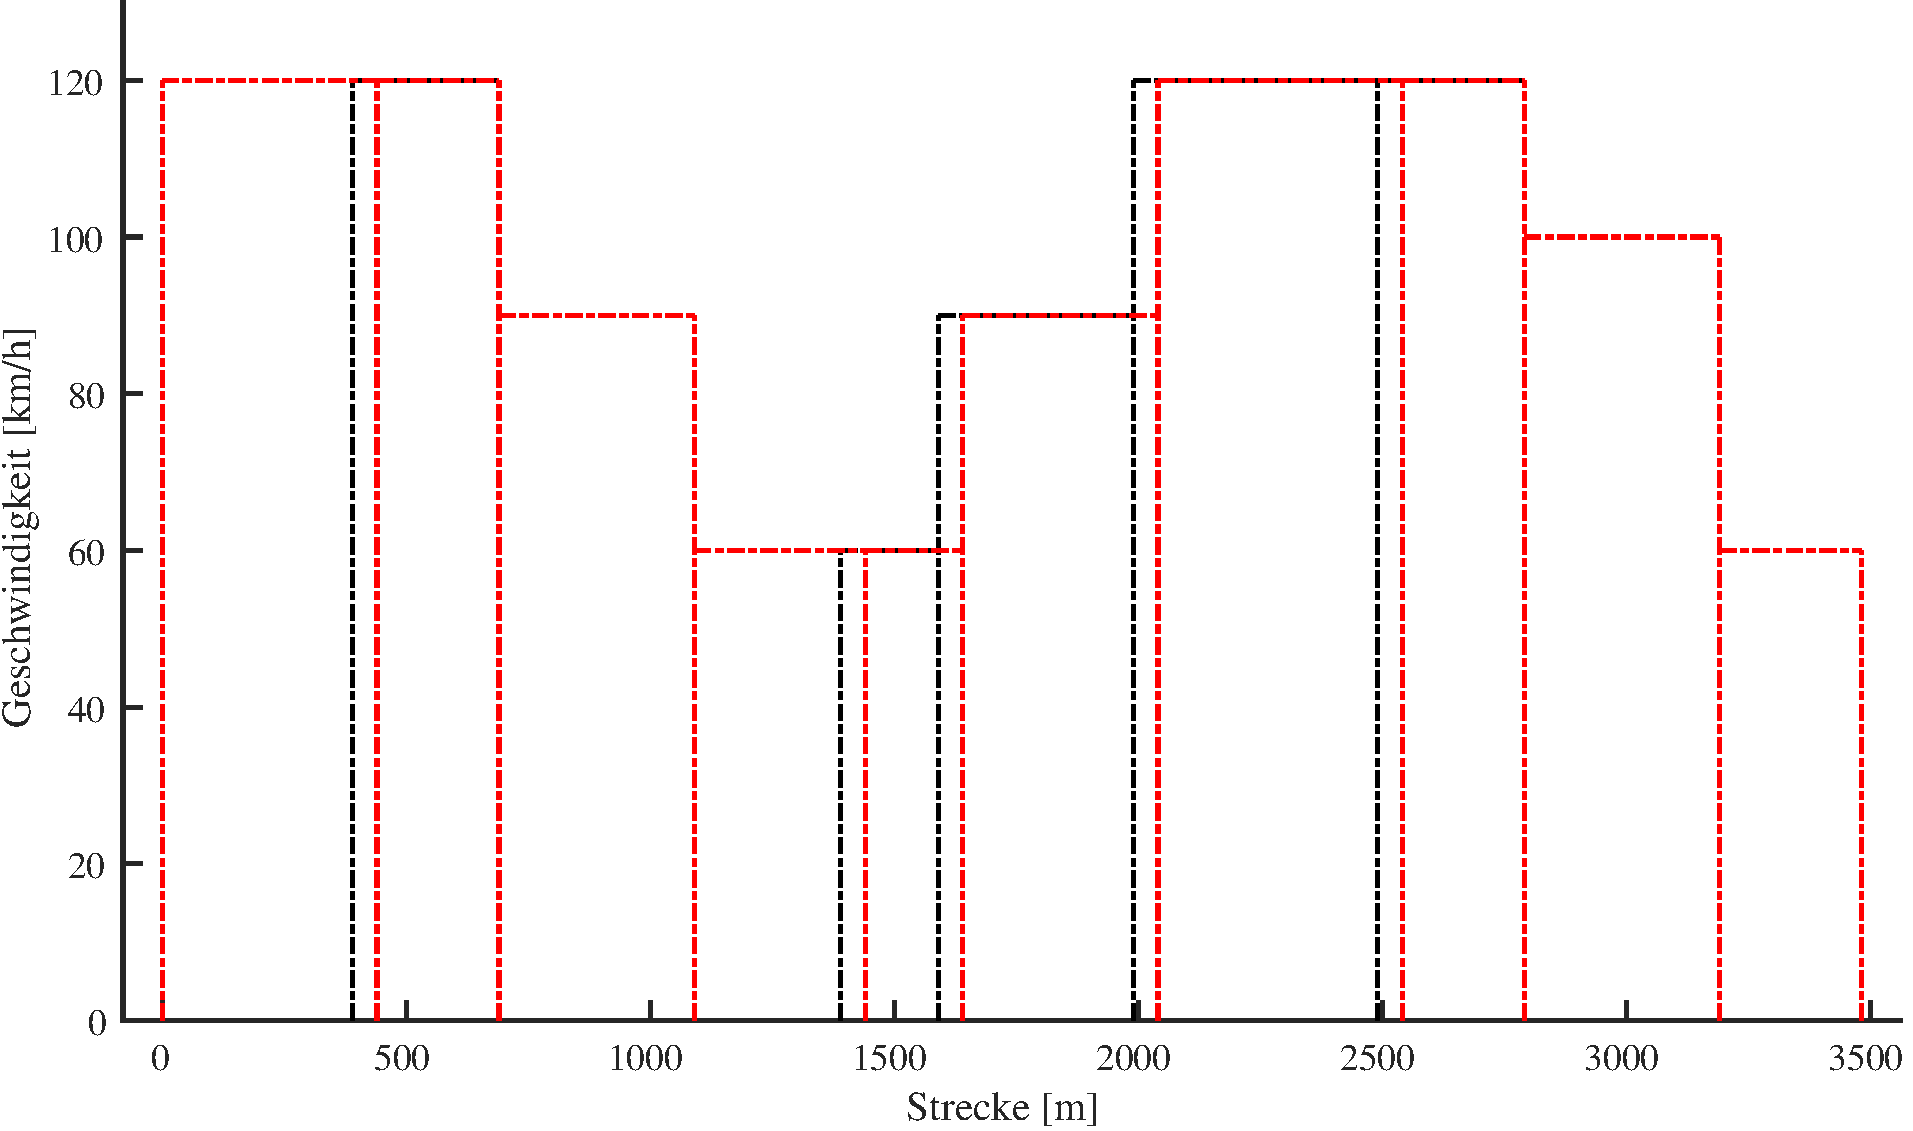
\includegraphics[width=\linewidth]{../images/matlab/it2.pdf}
\caption{Infra-Abschnitte und die zugehörige Höchstgeschwindigkeit unter Berücksichtigung der Fahrzeuglänge}
\label{fig:it2}
\end{figure}
\subsection{Berechnung bei einer Beschleunigung auf die maximal mögliche Geschwindigkeit} \label{v_max}
Im ersten Schritt der \Gls{fahrtverlauf}sberechnung wird die Distanz zwischen der aktuellen Position und der Ziel-Position mittels \textit{\$cumulativeSectionLengthStart}, \textit{\$cumulativeSectionLengthEnd}, \textit{\$indexCurrentSection} und \textit{\$indexTargetSection} berechnet. Für die Distanz und die Startgeschwindigkeit wird mit Hilfe der Funktion \textit{get\-V\-Max\-Be\-tween\-Two\-Points$($$)$} (\textit{func\-tions\_fahrt\-ver\-lauf.php}) (Code-Beispiel \ref{lst:getVMaxBetweenTwoPoints}) die maximale Geschwindigkeit ermittelt, auf die das Fahrzeug beschleunigen kann, um bis zum Ziel rechtzeitig bremsen zu können. Dabei wird in 10 $km/h$-Schritten iteriert und der maximale Wert zurückgegeben. Innerhalb der Funktion wir die Funktion \textit{getBrakeDistance$($$)$} (\textit{functions\_math.php}) (Code-Beispiel \ref{lst:getBrakeDistance}) aufgerufen, welche die benötigte Distanz für eine Beschleunigung bzw. Verzögerung berechnet und auf der Gleichung \ref{eq:s_v_ges} aus Kapitel \ref{formulaBeschleunigung} basiert.
\begin{figure}
\begin{lstlisting}[caption={\textit{getVMaxBetweenTwoPoints$($$)$} (\textit{functions\_fahrtverlauf.php})},captionpos=b,label={lst:getVMaxBetweenTwoPoints}]
// Ermittelt die maximale Geschwindigkeit zwischen zwei Punkten
function getVMaxBetweenTwoPoints(float $distance, int $v_0, int $v_1) {

	global $verzoegerung;
	global $globalFloatingPointNumbersRoundingError;

	$v_max = array();

	for ($i = 0; $i <= 120; $i = $i + 10) {
		if ((getBrakeDistance($v_0, $i, $verzoegerung) + getBrakeDistance($i, $v_1, $verzoegerung)) < ($distance + $globalFloatingPointNumbersRoundingError)) {
			array_push($v_max, $i);
		}
	}

	if (sizeof($v_max) == 0) {
		if ($v_0 == 0 && $v_1 == 0 && $distance > 0) {
			echo "Der zug müsste langsamer als 10 km/h fahren, um das Ziel zu erreichen.";
		} else {
			//emergencyBreak($id);
		}
	} else {
		if ($v_0 == $v_1 && max($v_max) < $v_0) {
			$v_max = array($v_0);
		}
	}

	return max($v_max);
}
\end{lstlisting}
\end{figure}

Durch die gegebene Startgeschwindigkeit und die größtmögliche Geschwindigkeit wird ein erster \Gls{fahrtverlauf} berechnet, wobei zwei \textit{\$keyPoints} erzeugt werden. Mithilfe der Funktion \textit{createTrainChanges$($$)$} (\textit{functions\_fahrtverlauf.php}) wird aus diesen beiden \textit{\$keyPoints} für jede Geschwindigkeitsveränderung die aktuelle absolute Position und Geschwindigkeit ermittelt. An den Positionen, an denen das Fahrzeug eine konstante Geschwindigkeit hat, wird in 1 Meter Abständen die absolute Position und die Geschwindigkeit gespeichert. Die ermittelten Daten werden in den Arrays \textit{\$trainPositionChange} und \textit{\$trainSpeedChange} gespeichert und sind in der Darstellung \ref{fig:it3} abgebildet.
\begin{figure}
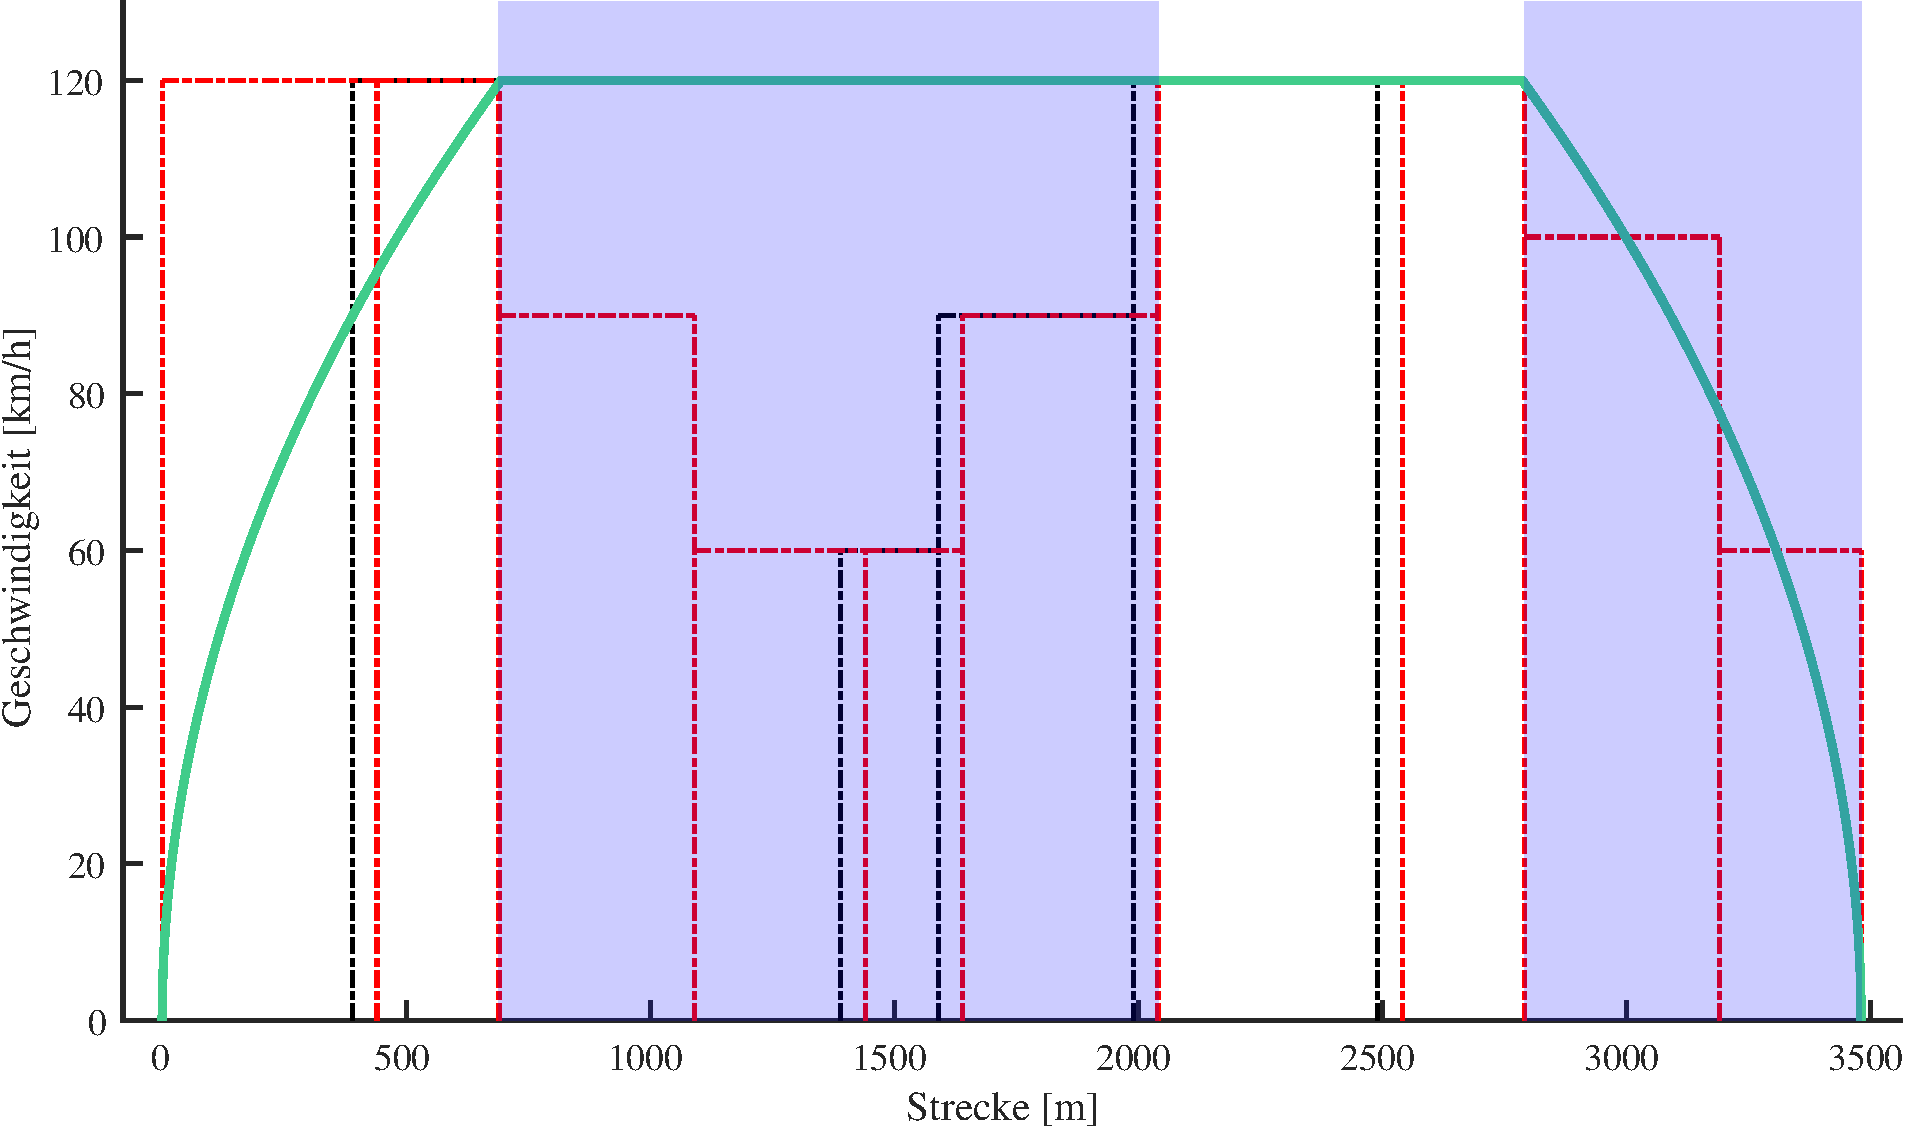
\includegraphics[width=\linewidth]{../images/matlab/it3.pdf}
\caption{\Gls{fahrtverlauf}sberechnung (1. Iterationsschritt)}
\label{fig:it3}
\end{figure}
\subsection{Überprüfung des \Gls{fahrtverlauf}s nach Geschwindigkeitsüberschreitungen} \label{überprüfung}
Für die Überprüfung, ob es bei einem \Gls{fahrtverlauf} zu einer Überschreitung der zulässigen Höchstgeschwindigkeit kommt, wird nach jeder Berechnung die Funktion \textit{check\-If\-Train\-Is\-To\-Fast\-In\-Certain\-Sec\-tions$($$)$} (\textit{functions\_fahrtverlauf.php}) (Code-Beispiel \ref{lst:checkIfTrainIsToFastInCertainSections}) aufgerufen. In dieser Funktion wird über alle absoluten Positionen (\textit{\$trainPositionChange}) iteriert, überprüft in welchem \ac{infra} sich diese Position befindet und überprüft, ob die zugehörige Geschwindigkeit aus dem \textit{\$trainSpeedChange}-Array die zulässige Höchstgeschwindigkeit überschreitet. Sobald in einem \ac{infra} eine Geschwindigkeitsüberschreitung vorliegt, wird der zugehörige Index des \ac{infra}s in dem \textit{\$faildSections}-Array gespeichert. Diese \ac{infra}e sind in der Darstellung \ref{fig:it3} Lila hinterlegt. 

Als Rückgabewert der Funktion wird ein Array zurückgegeben, welches abspeichert, ob und in welchen \ac{infra}en es zu einer Geschwindigkeitsüberschreitung gekommen ist (\textit{failed} und \textit{failed\_""sec\-tions}).
\begin{figure}
\begin{lstlisting}[caption={\textit{checkIfTrainIsToFastInCertainSections$($$)$} (\textit{func\-tions\_""fahrt\-ver\-lauf\-.php})},captionpos=b,label={lst:checkIfTrainIsToFastInCertainSections}]
// Überprüft, ob das Fahrzeug in Infra-Abschnitten die zulässige
// Höchstgeschwindigkeit überschreitet
function checkIfTrainIsToFastInCertainSections() {

	global $trainPositionChange;
	global $trainSpeedChange;
	global $cumulativeSectionLengthStartMod;
	global $next_v_max_mod;
	global $indexTargetSectionMod;

	$faildSections = array();

	foreach ($trainPositionChange as $trainPositionChangeKey => $trainPositionChangeValue) {
		foreach ($cumulativeSectionLengthStartMod as $cumulativeSectionLengthStartKey => $cumulativeSectionLengthStartValue) {
			if ($trainPositionChangeValue < $cumulativeSectionLengthStartValue) {
				if ($trainSpeedChange[$trainPositionChangeKey] > $next_v_max_mod[$cumulativeSectionLengthStartKey - 1]) {
					array_push($faildSections, ($cumulativeSectionLengthStartKey -1));
				}

				break;
			} else if ($cumulativeSectionLengthStartKey == $indexTargetSectionMod) {
				if ($trainPositionChangeValue > $cumulativeSectionLengthStartValue) {
					if ($trainSpeedChange[$trainPositionChangeKey] > $next_v_max_mod[$cumulativeSectionLengthStartKey]) {
						array_push($faildSections, $cumulativeSectionLengthStartKey);
					}

					break;
				}
			}
		}
	}

	if (sizeof($faildSections) == 0) {
		return array("failed" => false);
	} else {
		return array("failed" => true, "failed_sections" => array_unique($faildSections));
	}
}
\end{lstlisting}
\end{figure}
\subsection{Neuberechnung unter Berücksichtigung der Geschwindigkeitsüber-\\schreitung} \label{neuberechnung}
In dem Fall, dass es zu einer Geschwindigkeitsüberschreitung gekommen ist, wird der \Gls{fahrtverlauf} neu berechnet. Als Grundlage dafür dienen die \textit{failed\_sections} aus der \textit{check\-If\-Train\-Is\-To\-Fast\-In\-Certain\-Sections$($$)$}-Funktion (\textit{functions\_fahrtverlauf.php}) (Code-Beispiel \ref{lst:checkIfTrainIsToFastInCertainSections}). Die Funktion \textit{recalculate\-Key\-Points$($$)$} (\textit{functions\_fahrtverlauf.php}) vergleicht dabei immer zwei benachbarte \textit{\$keyPoints} und berechnet in dem Fall einer Geschwindigkeitsüberschreitung mit der Funktion \textit{check\-Between\-Two\-Key\-Points$($$)$} (\textit{func\-tions\_fahrt\-ver\-lauf\-.php}) diese neu. In dem Fall, dass zwischen zwei benachbarten \textit{\$keyPoints} die zulässige Höchst\-ge\-schwin\-dig\-keit überschritten wird, wird die absolute Start- und End-Position dieser Ge\-schwin\-digkeits\-über\-schrei\-tung gespeichert. 

In dem fol\-gen\-den Schritt wird wie in dem Abschnitt \ref{v_max} zwischen den Start-Werten des ersten \textit{\$keyPoints} und der ersten Geschwindigkeitsüberschreitung die maximale Geschwindigkeit berechnet und zwei neue \textit{\$keyPoints} erzeugt. Das gleiche passiert zwischen der Position der letzten Geschwindigkeitsüberschreitung und den End-Werten des zweiten \textit{\$keyPoints}. Dadurch wird sichergestellt, dass immer eine gerade Anzahl an \textit{\$keyPoints} existiert und somit in jedem Iterationsschritt zwei benachbarte \textit{\$keyPoints} verglichen werden können. Nachdem alle \textit{\$keyPoint}-Paare überprüft wurden, werden mit Hilfe der \textit{create\-Train\-Changes$($$)$}-Funktion (\textit{functions\_fahrtverlauf.php}) die Arrays \textit{\$train\-Position\-Change} und \textit{\$train\-Speed\-Change} erzeugt. Der neu berechnete \Gls{fahrtverlauf} wird erneut der Funktion \textit{check\-If\-Train\-Is\-To\-Fast\-In\-Certain\-Sections$($$)$} (\textit{func\-tions\_""fahrt\-ver\-lauf\-.php}) (Code-Bei\-spiel \ref{lst:checkIfTrainIsToFastInCertainSections}) übergeben. Dieser Prozess wird solange durchlaufen, bis es zu keiner Geschwindigkeitsüberschreitung mehr kommt. In den folgenden Abbildungen (Darstellung \ref{fig:it4}, \ref{fig:it5} und \ref{fig:it6}) werden die Ergebnisse der einzelnen Iterationsschritte visuell abgebildet, wobei die grau gepunkteten Linien die Ergebnisse der vorherigen Iterationsschritte darstellen.
\begin{figure}
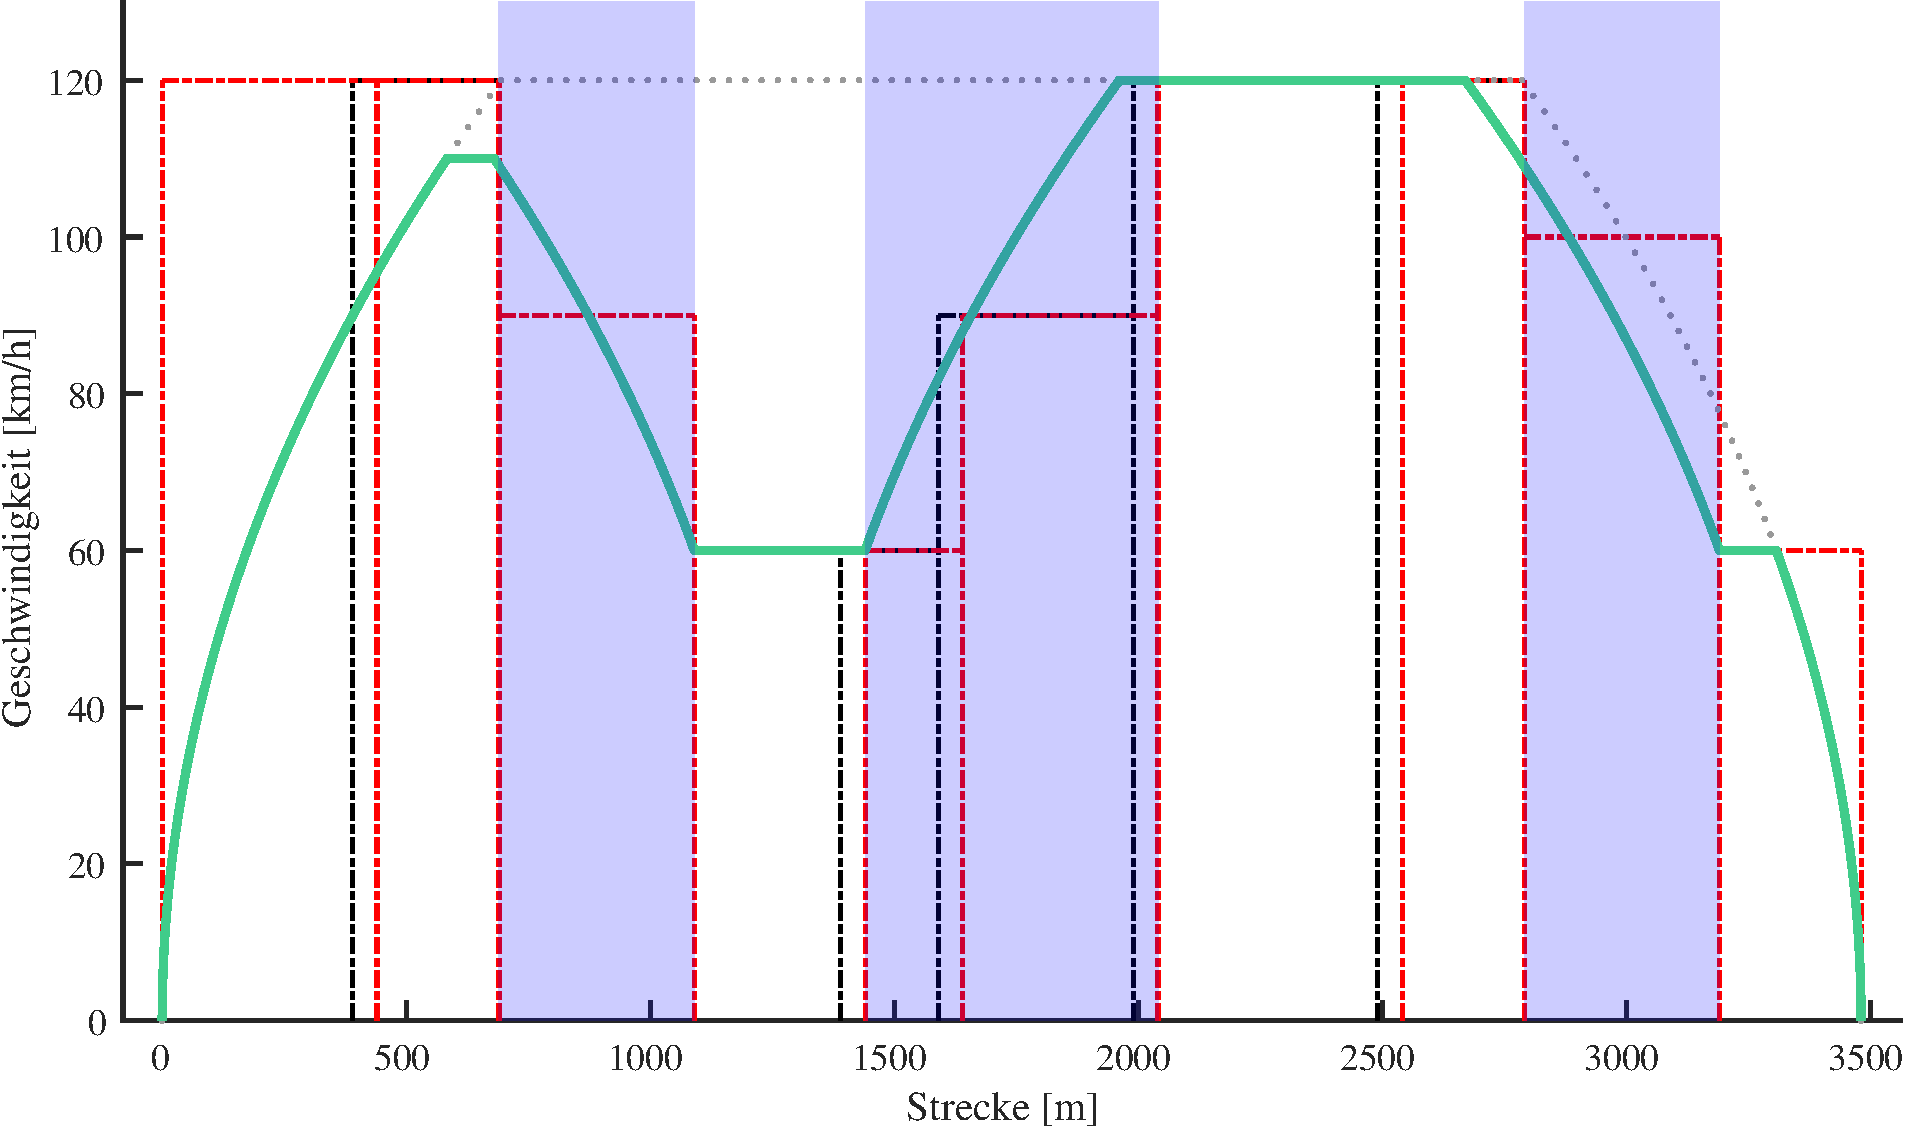
\includegraphics[width=\linewidth]{../images/matlab/it4.pdf}
\caption{\Gls{fahrtverlauf}sberechnung (2. Iterationsschritt)}
\label{fig:it4}
\end{figure}
\begin{figure}
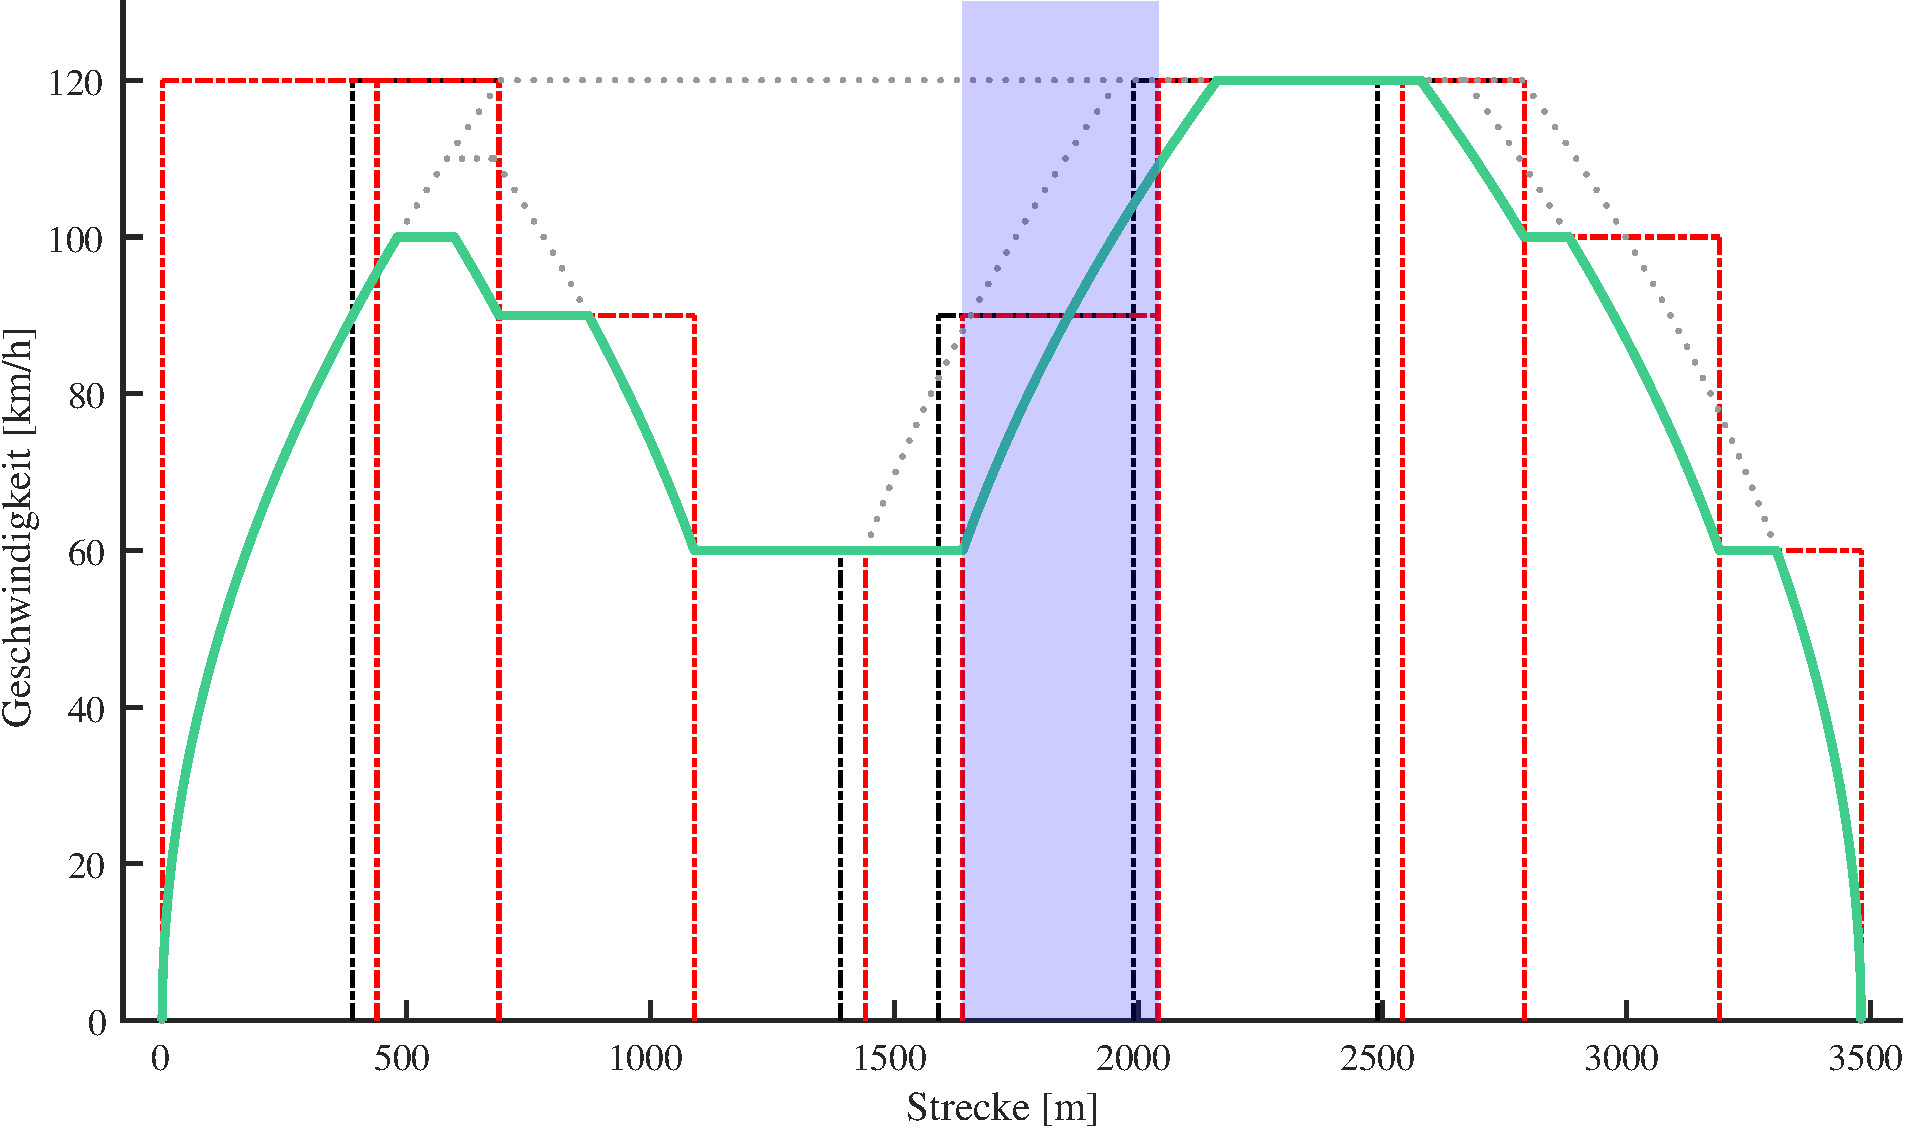
\includegraphics[width=\linewidth]{../images/matlab/it5.pdf}
\caption{\Gls{fahrtverlauf}sberechnung (3. Iterationsschritt)}
\label{fig:it5}
\end{figure}
\begin{figure}
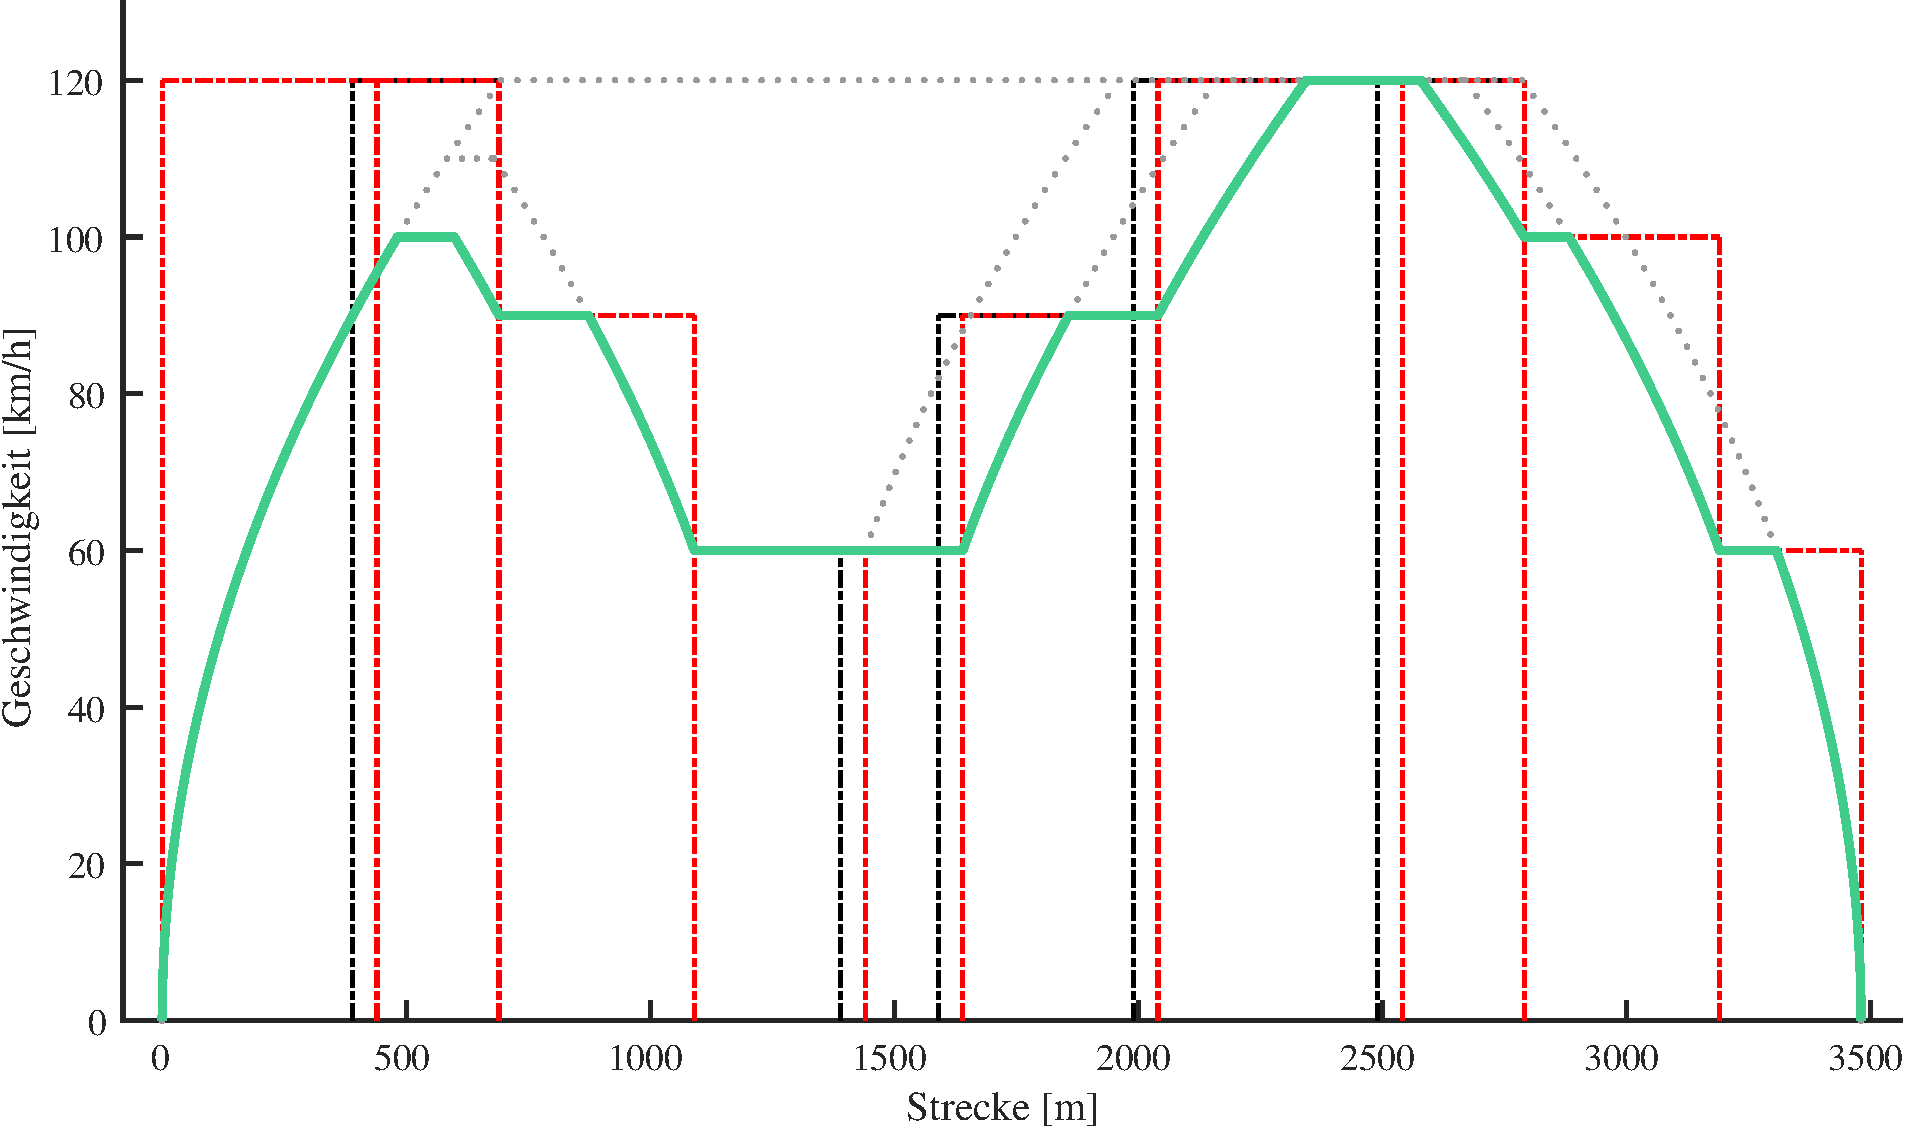
\includegraphics[width=\linewidth]{../images/matlab/it6.pdf}
\caption{\Gls{fahrtverlauf}sberechnung (4. Iterationsschritt)}
\label{fig:it6}
\end{figure}
\subsection{Einhaltung der Mindestzeit auf einer \Gls{beharrungsfahrt}} \label{minTime}
Für eine möglichst realitätsnahe Simulation kann über die Variable \textit{\$global\-Time\-On\-One\-Speed} in der Datei \textit{global\_variables.php} eine Mindestzeit festgelegt werden, die ein Fahrzeug auf einer Geschwindigkeit mindestens einhalten muss (\Gls{beharrungsfahrt}). Ebenfalls kann über die Variablen \textit{\$useMinTimeOnSpeed} und \textit{\$errorMinTimeOnSpeed} festgelegt werden, ob die Funktion aktiviert sein soll und ob es in dem Fall, dass diese Zeit nicht eingehalten werden kann, zu einer Fehlermeldung kommen soll. Im Falle einer Fehlermeldung würde das Fahrzeug nicht losfahren bzw. eine Gefahrenbremsung einleiten, falls das Fahrzeug aktuell eine Geschwindigkeit $v > 0$ $km/h$ hat. 

Wenn auf einem Abschnitt die Mindestzeit nicht eingehalten werden kann, kann eine Beschleunigung später eingeleitet werden, eine Verzögerung vorzeitiger eingeleitet werden oder auf eine kleinere Geschwindigkeit beschleunigt werden. Dadurch, dass sich eine Verschiebung einer Beschleunigung bzw. Verzögerung auf die nächsten Abschnitte auswirken kann, wird der \Gls{fahrtverlauf} in \textit{\$subsections} unterteilt. Eine \textit{\$subsection} beschreibt dabei den Bereich des \Gls{fahrtverlauf}s, in dem das Fahrzeug zum ersten Mal beschleunigt und zum letzten Mal abbremst. In der Darstellung \ref{fig:it7} wurde der exemplarische \Gls{fahrtverlauf} somit in zwei \textit{\$subsection} unterteilt, welche Lila bzw. Gelb hinterlegt sind.
\begin{figure}
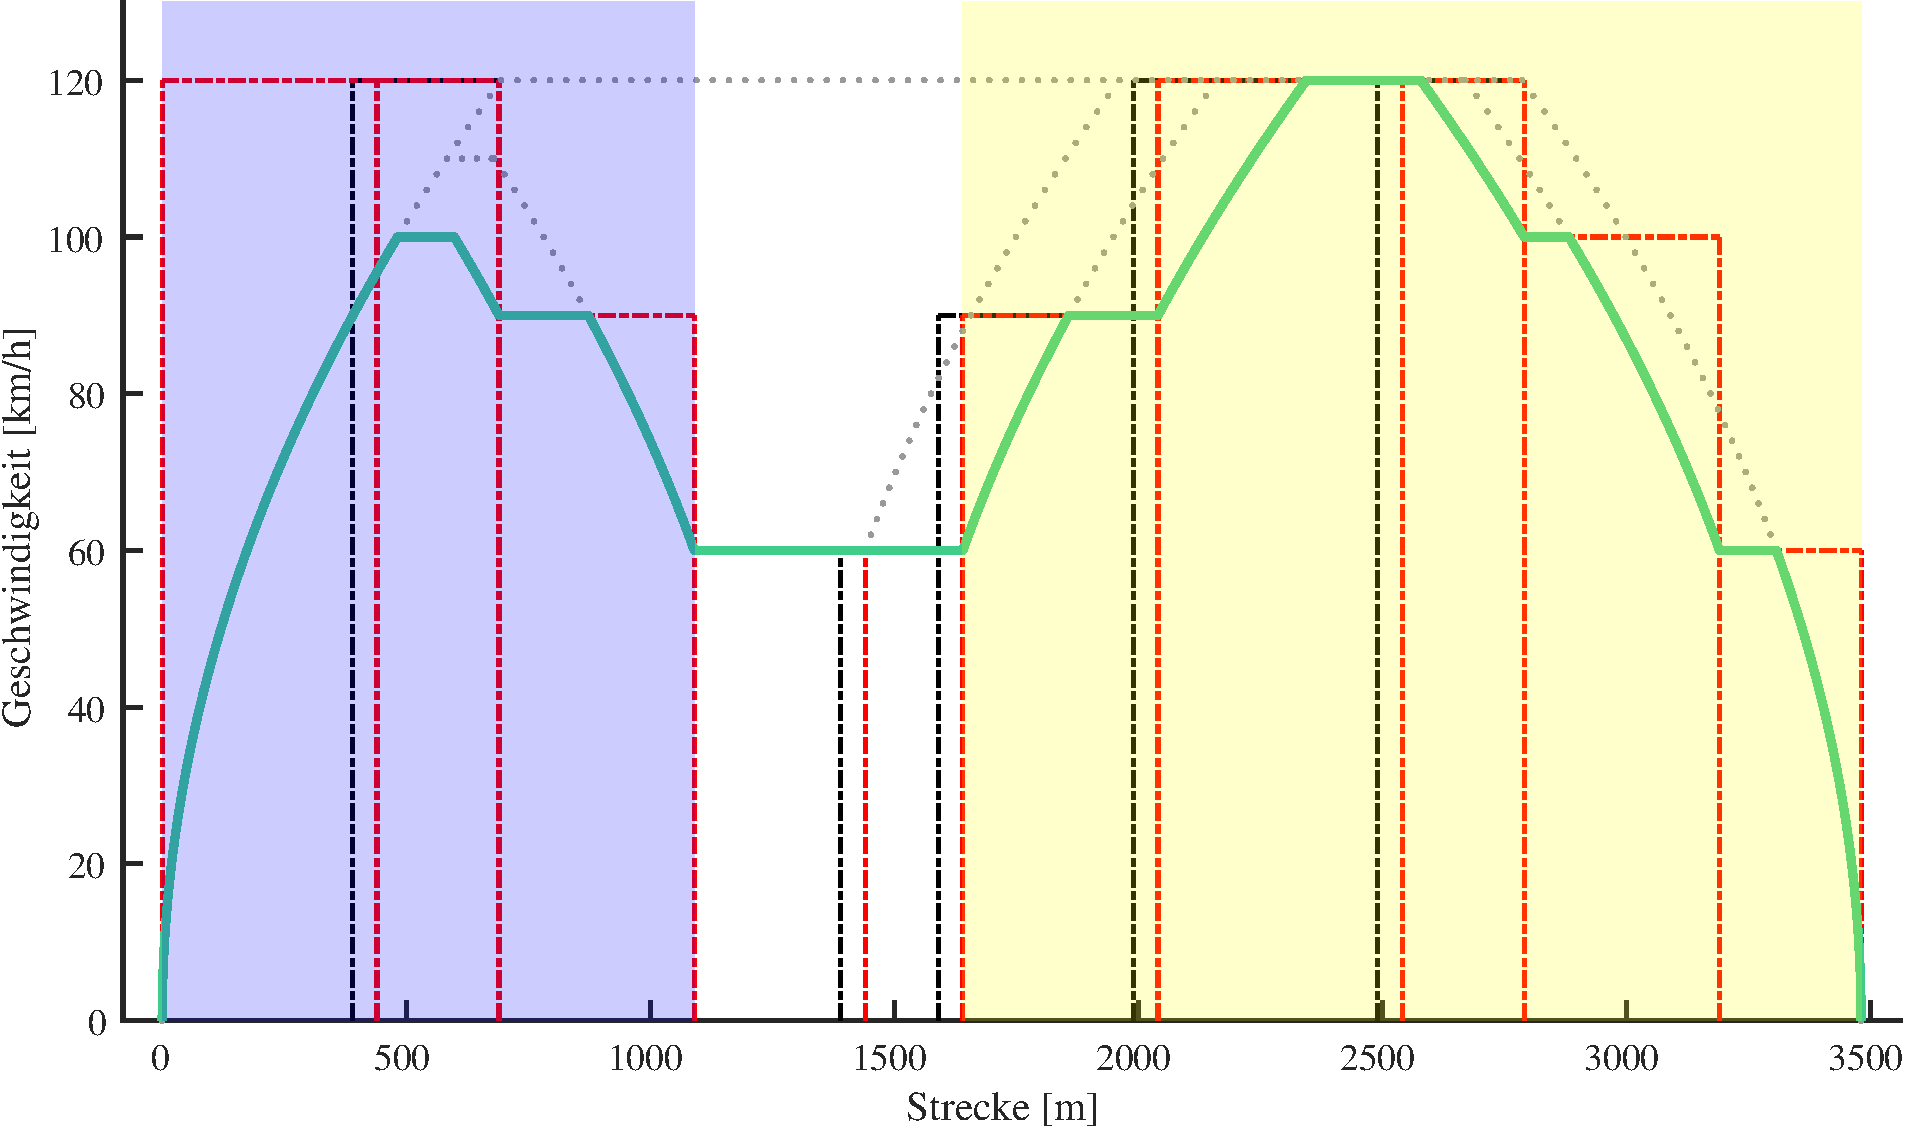
\includegraphics[width=\linewidth]{../images/matlab/it7.pdf}
\caption{Einteilung des \Gls{fahrtverlauf}s in \textit{\$subsections}}
\label{fig:it7}
\end{figure}
Durch diese Einteilung kann verhindert werden, dass es zu Konflikten kommt. Falls die Beschleunigungen bzw. Verzögerungen soweit nach hinten bzw. nach vorne verschoben werden müssen, kann die maximale Geschwindigkeit auf dieser \textit{\$subsection} reduziert werden und die zur Verfügung stehende Strecke vergrößert werden. Wie in Darstellung \ref{fig:it7} zu erkennen wird hierbei im ersten Schritt der Abschnitt zwischen zwei \textit{\$subsections} ausgelassen. Nach der Ermittlung der \textit{\$subsections} wird überprüft, ob auf den Abschnitten zwischen den \textit{\$subsections} die Mindestzeit eingehalten wird. Wenn das nicht der Fall ist, wird der Abschnitt automatisch der in Fahrtrichtung hinteren \textit{\$subsection} zugeordnet. Dadurch wird sichergestellt, dass das Fahrzeug, wenn es an einer Stelle des \Gls{fahrtverlauf}s die Geschwindigkeit reduziert, dies möglichst spät tut.

Nachdem die \textit{\$subsections} mittels der Funktion \textit{createSubsections$($$)$} (\textit{func\_tions\_""fahrt\-ver\-lauf.php}) erstellt wurden und mit der Funktion \textit{array\_reverse$($$)$} in umgekehrter Reihenfolge in dem Array \textit{\$subsection\_list} gesammelt wurden, wurde für jede \textit{\$subsection} ein Array erzeugt, welches die Variablen aus Tabelle \ref{table:subsection} beinhaltet und jede \textit{\$subsection} eindeutig beschreibt.
\begin{table}
\begin{center}
\renewcommand{\arraystretch}{1.2}
\begin{tabular}{c|c}
Index & Funktion \\ \hline
\textit{max\_index}                 	&  	\makecell{Index des \textit{\$keyPoints} mit der Beschleunigung auf die\\maximale Geschwindigkeit in der \textit{\$subsection}}     \\ \hline
\textit{indexes} (Array)                 		&    	Indexe aller beinhalteten \textit{\$keyPoints}                  \\ \hline
\makecell{\textit{is\_prev\_section}\\(Boolescher Wert)}           	&   	Berücksichtigung des Abschnitts vor der \textit{\$subsection}     \\ \hline
\makecell{\textit{is\_next\_section}\\(Boolescher Wert)}           	&     	Berücksichtigung des Abschnitts nach der \textit{\$subsection}                 \\ \hline
\textit{failed} (Boolescher Wert)             & Unterschreitung der Mindestzeit auf der \textit{\$subsection}     \\ 
\end{tabular}
\renewcommand{\arraystretch}{1}
\caption{Aufbau des \textit{\$subsection}-Arrays}
\label{table:subsection}
\end{center}
\end{table}

Bei den \textit{\$subsections}, bei denen die Mindestzeit für die \Gls{beharrungsfahrt}en nicht eingehalten wird (\textit{failed} == \textit{true}), wird überprüft, ob eine Verschiebung der Beschleunigungen bzw. Verzögerungen möglich ist. Bei der Verschiebung einer Beschleunigung bzw. Verzögerung wird die Differenz zwischen der Mindestzeit einer \Gls{beharrungsfahrt} (\textit{\$global\-Time\-On\-One\-Speed}) und der Zeit der vorherigen bzw. folgenden \Gls{beharrungsfahrt} berechnet und die Beschleunigung bzw. Verzögerung um diese Differenz verschoben.

Sollte bei einer Verschiebung die \textit{position\_1} eines \textit{\$keyPoints} hinter \textit{position\_0} des folgenden \textit{\$keyPoints} liegen (bei einer Beschleunigung), wird der zweite \textit{\$keyPoint} gelöscht und die Zielgeschwindigkeit des zweiten \textit{\$keyPoints} wird der Zielgeschwindigkeit des ersten \textit{\$keyPoints} zugewiesen. Gleiches geschieht bei der Verzögerung in umgekehrter Reihenfolge. 

Nach der Verschiebung wird überprüft, ob auf allen konstanten Geschwindigkeit die Mindestzeit eingehalten wird. Wenn das der Fall ist, wird die nächste \textit{\$subsection} überprüft. In dem Fall, dass durch die Verschiebung die Mindestzeit nicht eingehalten werden kann, wird die maximale Geschwindigkeit auf dieser \textit{\$subsection} um 10 $km/h$ reduziert, die \textit{\$subsections} neu berechnet und erneut über alle \textit{\$subsection} iteriert. Die Neuberechnung ist notwendig, da durch die Reduzierung der Geschwindigkeit die \textit{\$subsections} anders aufgeteilt sein können.

Wenn alle \textit{\$subsections} die Mindestzeit einhalten, wird der Algorithmus beendet. In der Darstellung \ref{fig:it9} ist der \Gls{fahrtverlauf} unter Einhaltung der Mindestzeit auf einer Geschwindigkeit abgebildet.
\begin{figure}
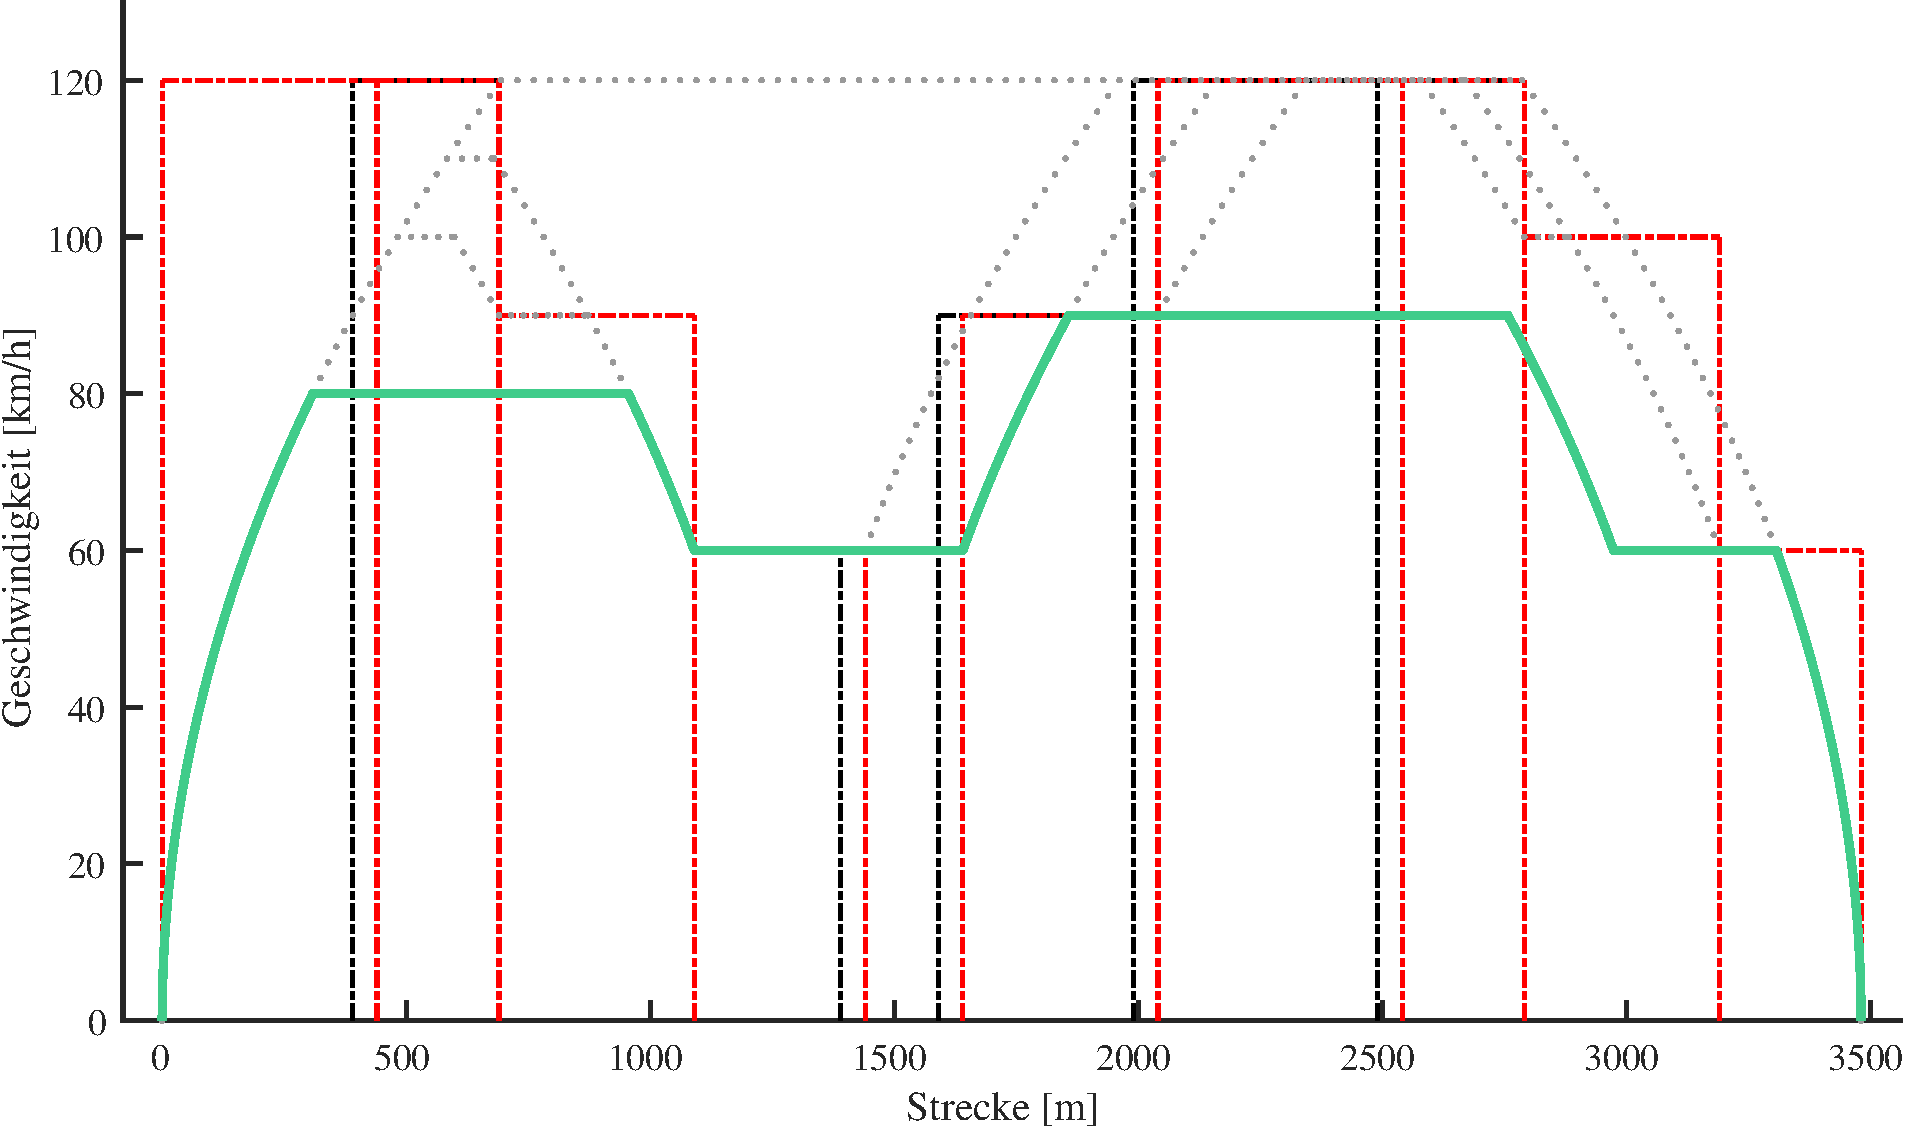
\includegraphics[width=\linewidth]{../images/matlab/it9.pdf}
\caption{\Gls{fahrtverlauf} unter Einhaltung der Mindestzeit}
\label{fig:it9}
\end{figure}
Für den Fall, dass das Fahrzeug auf einer Geschwindigkeit die Mindestzeit nicht einhält und als nächstes beschleunigen würde, kann die Beschleunigung später eingeleitet werden. 

\subsection{Berücksichtigung der Ankunftszeit bei der Berechnung des \Gls{fahrtverlauf}s} \label{time}
Der berechnete \Gls{fahrtverlauf} aus den Kapiteln \ref{v_max}, \ref{überprüfung}, \ref{neuberechnung} und \ref{minTime} ermittelt die frühstmögliche Ankunftszeit am Ziel. In dem Fall, dass der Zug dadurch mit einer Verspätung am Ziel ankommt, wird der \Gls{fahrtverlauf} an das Fahrzeug übergeben. Falls das Fahrzeug mit dem \Gls{fahrtverlauf} zu früh am Ziel ankommen würde, wird überprüft, ob es möglich ist die Geschwindigkeit zu reduzieren, sodass der Zug energieeffizienter fahren kann und ohne Verspätung am Ziel ankommt. 

Im ersten Schritt wird mittels der Funktion \textit{check\-If\-The\-Speed\-Can\-Be\-De\-creased$($$)$} (\textit{func\-tions\_""fahrt\-ver\-lauf\-.php}) überprüft, ob die Geschwindigkeit reduziert werden kann. Dabei werden alle \textit{\$keyPoints} ermittelt, bei denen das Fahrzeug beschleunigt und die beim darauffolgenden \textit{\$keyPoint} abbremsen. Für jeden dieser \textit{\$keyPoints} werden die möglichen Geschwindigkeiten ermittelt, welche das Fahrzeug zwischen den beiden \textit{\$keyPoints} fahren könnte. Für die Berechnung dieser Geschwindigkeiten wird als niedrigste Geschwindigkeit die \textit{speed\_0} des ersten \textit{\$keyPoints} bzw. \textit{speed\_1} des zweiten \textit{\$keyPoints} -- jenachdem, welche niedriger ist -- genommen und in 10 $km/h$-Schritten bis  \textit{speed\_1} des ersten \textit{\$keyPoints} abgespeichert. Daraus ergibt sich für jeden \textit{\$keyPoint} eine \textit{range} an möglichen Geschwindigkeiten. Als Rückgabewert der Funktion wird ein Array zurückgegeben, welches die Einträge \textit{possible} und \textit{range} enthält und als \textit{\$return\-Speed\-Decrease} abgespeichert. Der Eintrag \textit{possible} gibt an, ob das Fahrzeug auf dem gesamten \Gls{fahrtverlauf} die Geschwindigkeit reduzieren könnte und wird als Boolescher Wert (\textit{true}/\textit{false}) abgespeichert und in dem Array \textit{range} werden alle Indexe der möglichen \textit{\$keyPoints} inklusive der ermittelten Geschwindigkeiten abgespeichert.

In dem in Abbildung \ref{fig:it9} dargestellten \Gls{fahrtverlauf} wären für den \textit{\$keyPoint} mit dem Index 0 (die Indexe der \textit{\$keyPoints} entsprechen dem Zahlenbereich der $\mathbb{N}_0$) die Geschwindigkeiten 60, 70 und 80 $km/h$ ermittelt worden und für den \textit{\$keyPoint} mit dem Index 2 die Geschwindigkeiten 60, 70, 80 und 90 $km/h$.

Wenn eine Reduzierung der Geschwindigkeit möglich ist, wird in einer \textit{while}-Schleife versucht die Geschwindigkeit zu reduzieren, bis das Fahrzeug bei der nächsten Reduzierung mit einer Verspätung am Ziel ankommen würde oder eine weitere Reduzierung nicht möglich ist. Innerhalb der \textit{while}-Schleife ermittelt die Funktion \textit{find\-Max\-Speed$($$)$} (\textit{functions\_fahrtverlauf.php}) aus dem \textit{\$returnSpeedDecrease}-Array den \textit{\$keyPoint} mit der höchsten Geschwindigkeit. Für den Fall, dass mehrere \textit{\$keyPoints} die selbe Höchstgeschwindigkeit haben, wird der letzte dieser \textit{\$keyPoints} ermittelt. Im Anschluss wird mit einer \textit{for}-Schleife in 10 $km/h$-Schritten in absteigender Reihenfolge über die möglichen Geschwindigkeiten iteriert und überprüft, ob durch die Anpassung die Ankunftszeit eingehalten werden kann. Sobald die Ankunftszeit nicht eingehalten werden kann, werden die \textit{\$keyPoints} aus dem vorherigen Iterationsschritt gespeichert und die \textit{while}-Schleife wird abgebrochen. Sollte die \textit{for}-Schleife durchlaufen, ohne dass es zu einer Überschreitung der maximal verfügbaren Zeit kommt, wird die Funktion \textit{checkIfTheSpeedCanBeDecreased$($$)$} (\textit{functions\_fahrtverlauf.php}) erneut aufgerufen. 
Das Ergebnis dieser Berechnung ist in der Abbildung \ref{fig:it10} abgebildet.
\begin{figure}
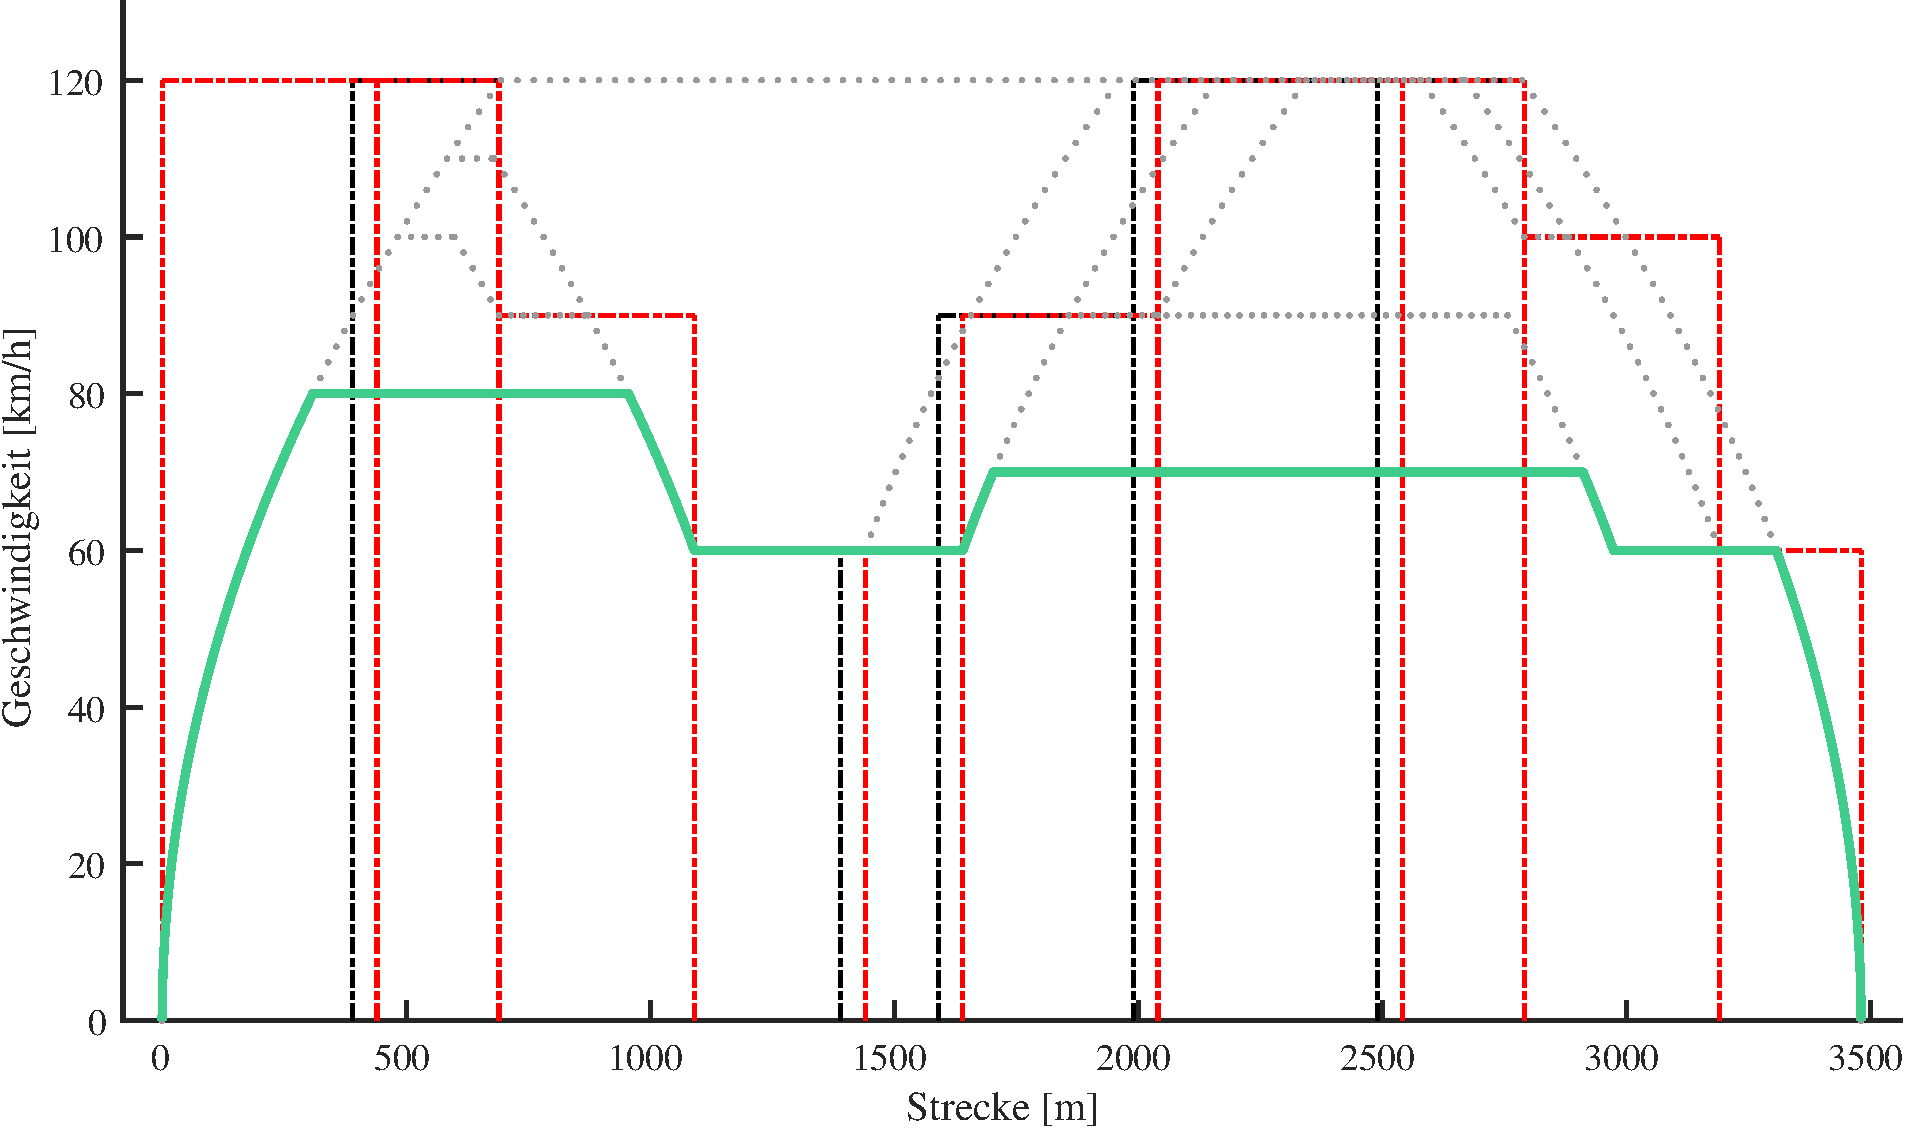
\includegraphics[width=\linewidth]{../images/matlab/it10.pdf}
\caption{\Gls{fahrtverlauf} mit reduzierter Geschwindigkeit unter Einhaltung der An\-kunfts\-zeit}
\label{fig:it10}
\end{figure}
\subsection{Berücksichtigung der exakten Ankunftszeit bei der Berechnung des \Gls{fahrtverlauf}s} \label{time2}
Die in Kapitel \ref{minTime} errechnete Ankunftszeit, beschreibt die spätmöglichste Ankunftszeit am Ziel, ohne dass das Fahrzeug mit einer Verspätung am Ziel ankommt, wenn bei einer Beschleunigung auf eine geringere Zielgeschwindigkeit beschleunigt wird. Dadurch wird das Fahrzeug im Normalfall nicht exakt pünktlich das Ziel erreichen. Über die Variable \textit{\$useSpeedFineTuning} kann festgelegt werden, ob das Fahrzeug eine exakte Ankunftszeit versuchen soll zu erreichen. Wenn diese Funktion aktiviert ist und der Eintrag \textit{possible} aus dem Array \textit{\$returnSpeedDecrease} \textit{true} ist, wird für den letzten \textit{\$keyPoint} aus dem \textit{\$return\-Speed\-De\-crease}-Array überprüft, ob die Verzögerung des nächsten \textit{\$keyPoints} vorzeitiger eingeleitet werden kann. Sollte die Zielgeschwindigkeit der Verzögerung 0 $km/h$ sein, wird die Verzögerung unterteilt in eine Verzögerung auf 10 $km/h$ und eine von 10 $km/h$ auf 0 $km/h$. Die Position der vorzeitig eingeleiteten Verzögerung wird mittels der Funktion \textit{speedFineTuning$($$)$} (\textit{functions\_fahrtverlauf.php}) berechnet, welche als Parameter den Betrag der Differenz zwischen aktueller Soll- und Ist-Ankunftszeit und den Index des vorherigen \textit{\$keyPoints} übergeben bekommt und auf der Gleichung \ref{eq:t_1_tuning} aus Kapitel \ref{formula} basiert.
\begin{figure}
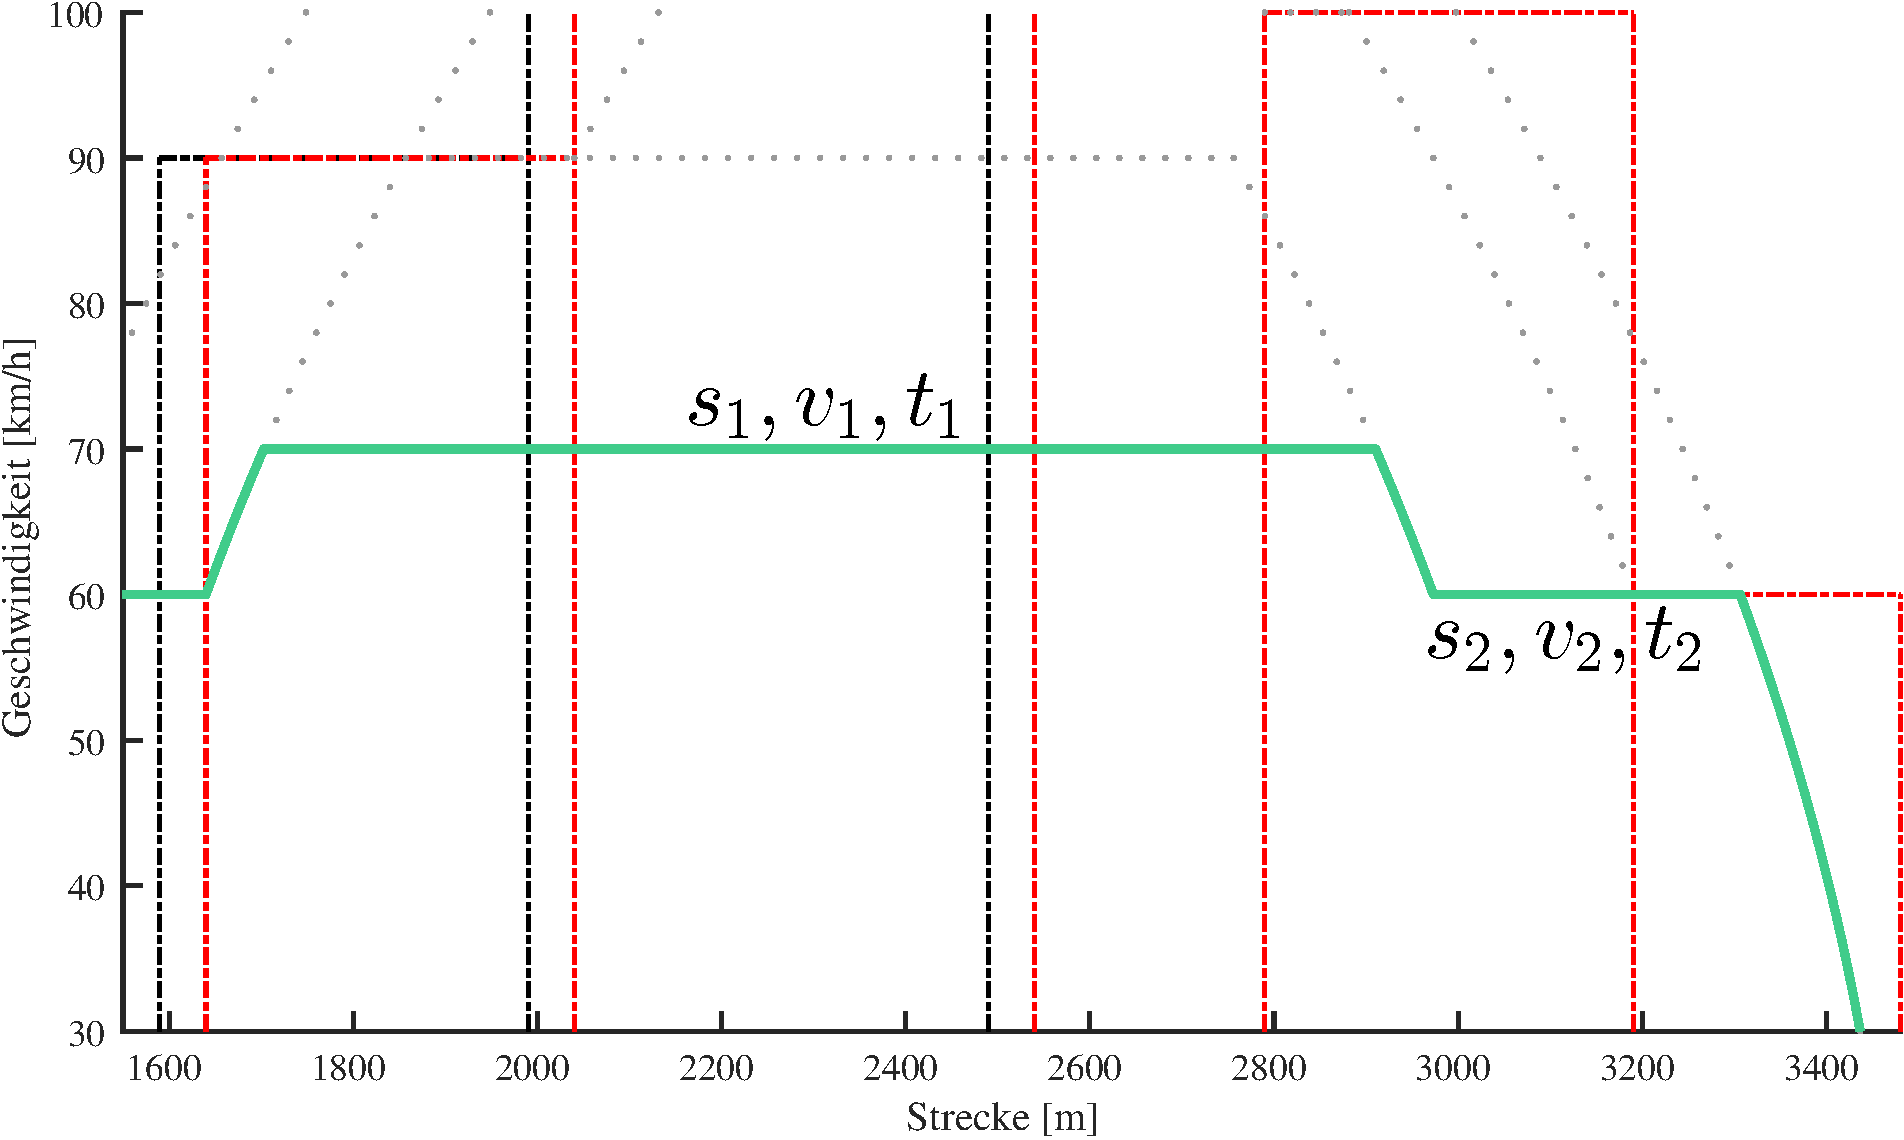
\includegraphics[width=\linewidth]{../images/matlab/it11.pdf}
\caption{\Gls{fahrtverlauf} vor der Anpassung der exakten Ankunftszeit}
\label{fig:it11}
\end{figure}
In Abbildung \ref{fig:it11} werden die Geschwindigkeiten ($v_1$, $v_2$), Strecken ($s_1$, $s_2$) und Zeiten ($t_1$, $t_2$) vor und nach der Verzögerung -- welche vorzeitiger eingeleitet werden soll, um eine pünktliche Ankunft am Ziel zu ermöglichen -- dargestellt und in Tabelle \ref{table:speed_fine_tuning_ex} sind die exakten Werte des exemplarischen \Gls{fahrtverlauf}s aufgelistet. In diesem konkreten Beispiel würde das Fahrzeug 3,31 $s$ ($t_{\varDelta}$) zu früh an der Betriebsstelle ankommen, wodurch das Fahrzeug für die Zurücklegung der Strecken $s_1$ und $s_2$ insgesamt 85,42 $s$ ($t_{ges}=t_1+t_2+t_{\varDelta}$) zur Verfügung hat.
\begin{table}
\begin{center}
\renewcommand{\arraystretch}{1.2}
\begin{tabular}{r l}
$v_1$                   &   70 $km/h$ ($\approx$ 19,44 $m/s$)                         \\ 
$v_2$                   &   60 $km/h$ ($\approx$ 16,67 $m/s$)                         \\ 
$s_1$                   &   1207,67 $m$                         \\ 
$s_2$                   &   333,33 $m$                         \\ 
$s_{ges}$                   &   1541 $m$                         \\ 
$t_1$                   &   62,11 $s$                         \\ 
$t_2$                   &   20 $s$                         \\ 
$t_{\varDelta}$                   &   3,31 $s$                         \\ 
$t_{ges}$                   &   85,42 $s$                         \\ 
\end{tabular}
\renewcommand{\arraystretch}{1}
\caption{Geschwindigkeiten, Strecken und Zeiten vor und nach der Verzögerung vor der Anpassung}
\label{table:speed_fine_tuning_ex}
\end{center}
\end{table}

Durch das Einsetzen der Werte in die Gleichung \ref{eq:t_1_tuning} aus dem Kapitel \ref{formulaGleichfoermig} ergibt sich für $t_3$ ($t_3$, $t_4$, $s_3$ und $s_4$ bezeichnen die Strecken und Zeiten nach der Anpassung) ein Wert von 42,2 $s$. Dementsprechend muss die Verzögerung 19,85 $s$ ($t_1$ - $t_3$) früher eingeleitet werden.
\begin{figure}[H]
\[t_{3} = \frac{1541\:m - 16,67\:m/s \cdot 85,42\:s}{19,44\:m/s - 16,67\:m/s}\]
%\[t_{3} = \frac{1541m - 1423,95 m}{2,77 m/s}\]
%\[t_{3} = \frac{117,05 m}{2,77 m/s}\]
\[t_{3} = 42,26\:s\]
\end{figure}
Die vorzeitige Einleitung der Verzögerung sorgt dafür, dass das Fahrzeug die nächste Betriebsstelle genau pünktlich erreicht und ist in Abbildung \ref{fig:it12} dargestellt, wobei durch die gepunktete Linie der \Gls{fahrtverlauf} vor der Anpassung zu sehen ist. Die neu berechneten Werte sind in Tabelle \ref{table:speed_fine_tuning_ex_2} aufgelistet.
\begin{figure}
  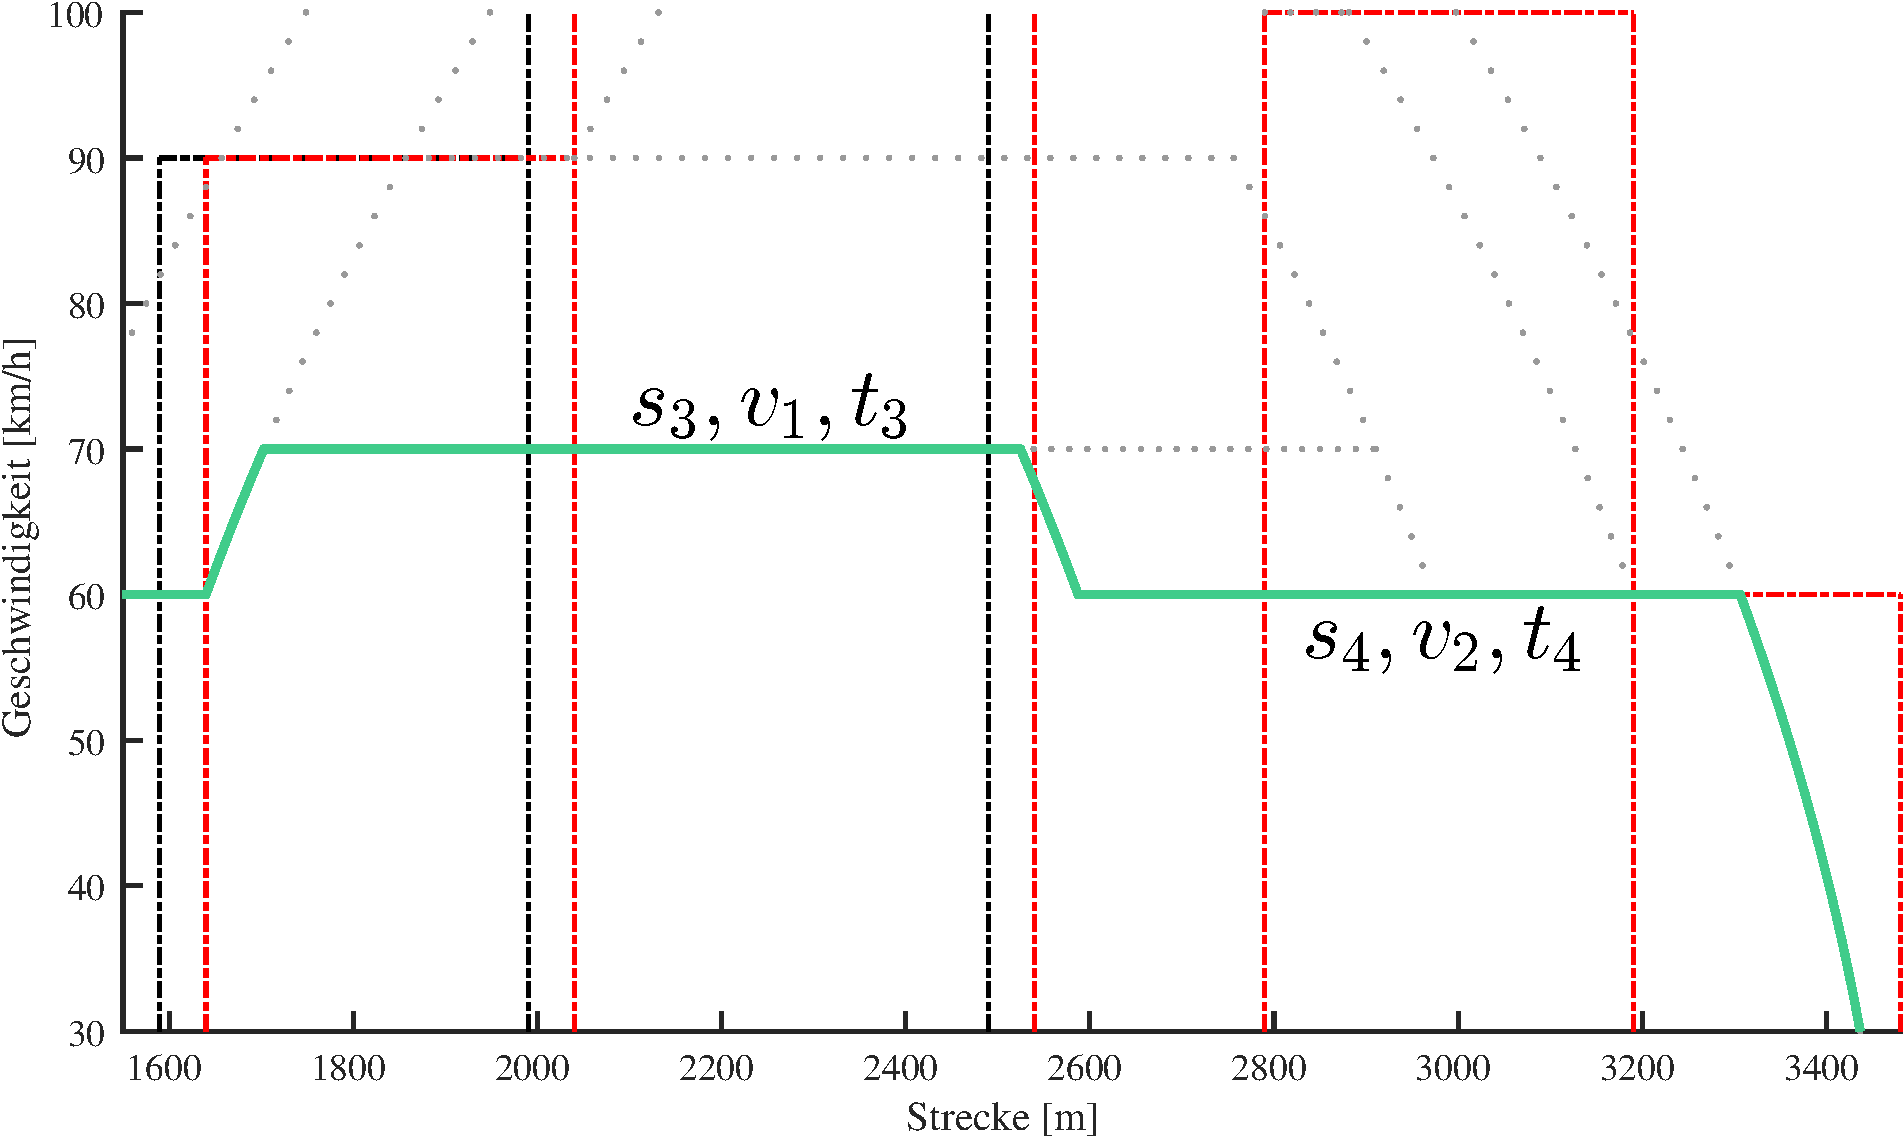
\includegraphics[width=\linewidth]{../images/matlab/it12.pdf}
  \caption{\Gls{fahrtverlauf} nach der Anpassung der exakten Ankunftszeit}
  \label{fig:it12}
\end{figure}
\begin{table}
\begin{center}
\renewcommand{\arraystretch}{1.2}
\begin{tabular}{r L{3cm}}
$s_3$                   	&   821,91 $m$                      	\\ 
$s_4$                   	&   719,1 $m$                         	\\ 
$t_3$                   	&   42,26 $s$                         	\\ 
$t_4$                   	&   43,16 $s$                         	\\ 
%$t_{ges}$           	&   85,42 $s$                         	\\ 
\end{tabular}
\renewcommand{\arraystretch}{1}
\caption{Geschwindigkeiten, Strecken und Zeiten vor und nach der Verzögerung nach der Anpassung}
\label{table:speed_fine_tuning_ex_2}
\end{center}
\end{table}
Der finale \Gls{fahrtverlauf} ist in Abbildung \ref{fig:it13} dargestellt und kann so dem Fahrzeug übergeben werden.
\begin{figure}
  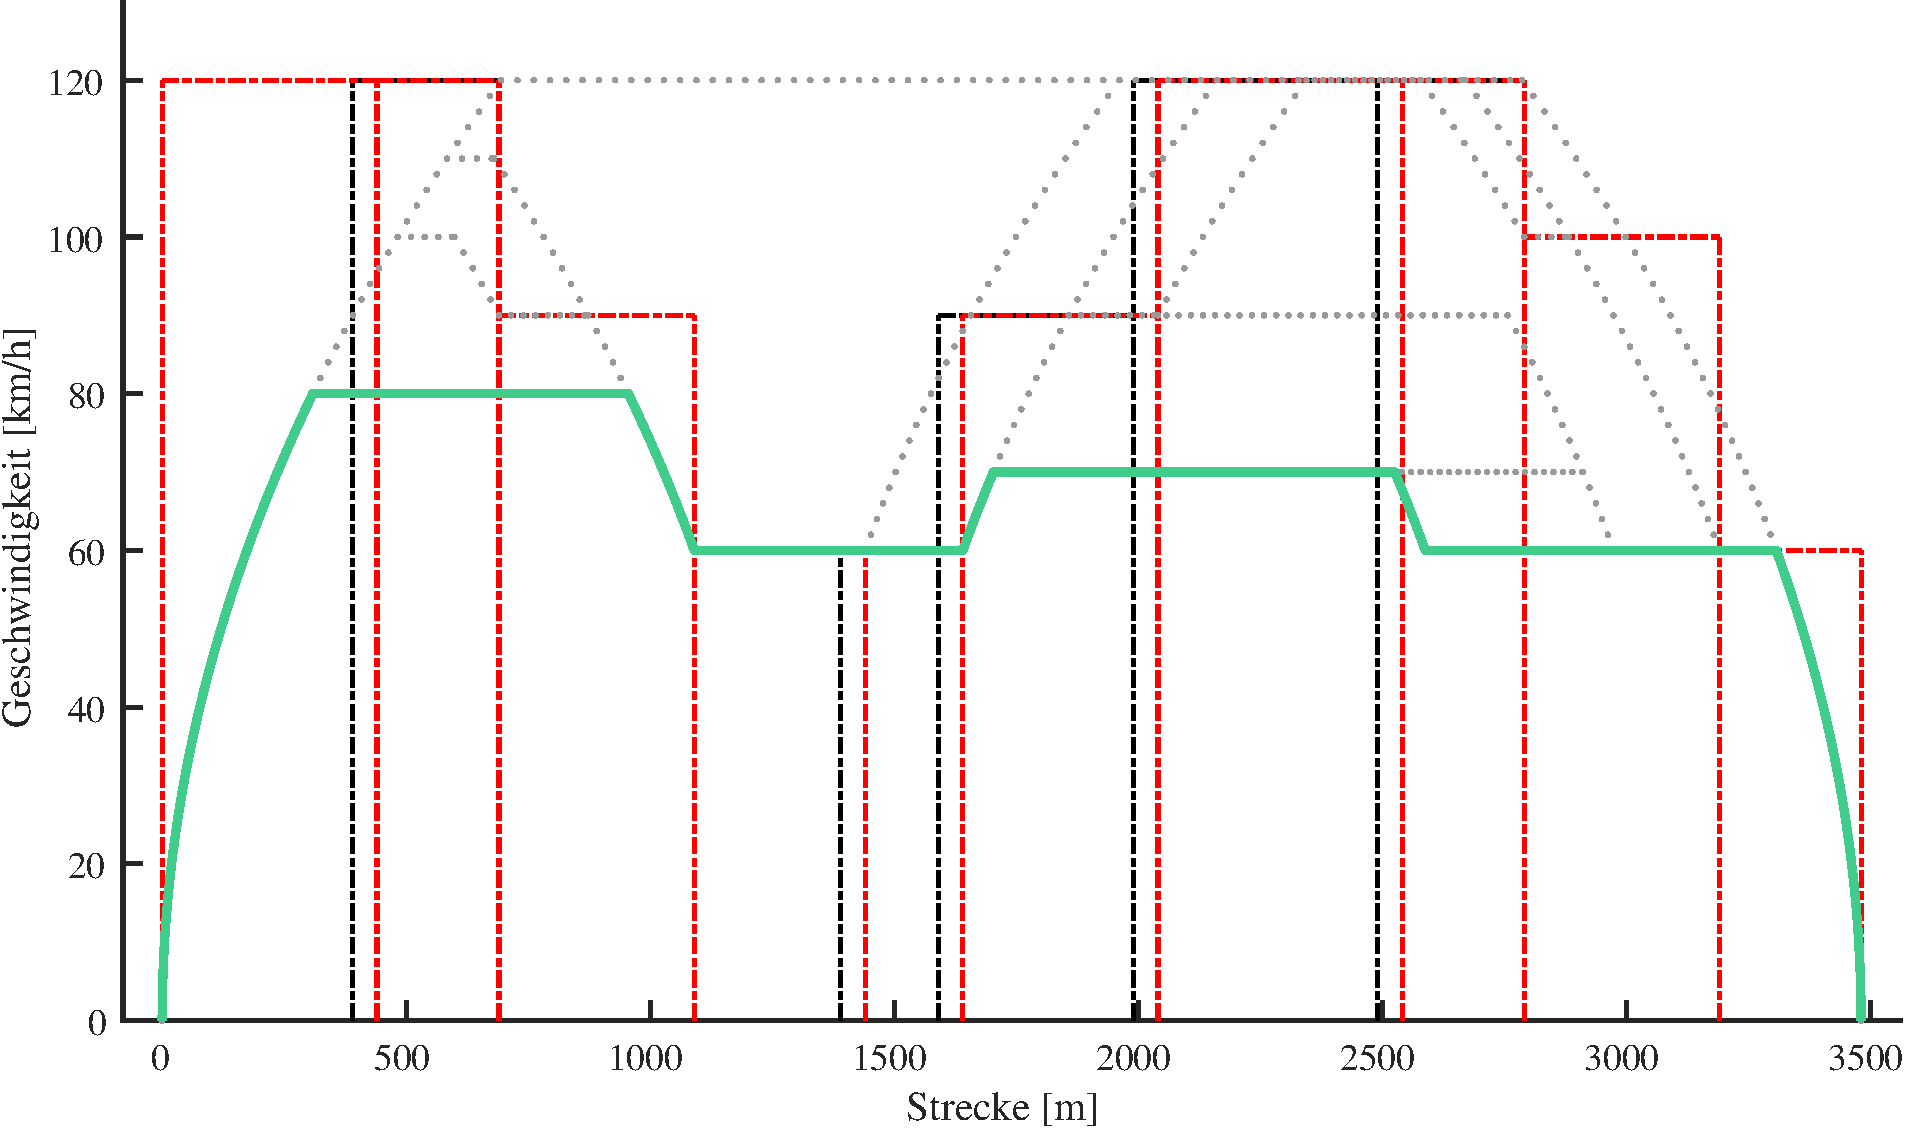
\includegraphics[width=\linewidth]{../images/matlab/it13.pdf}
  \caption{Ergebnis der \Gls{fahrtverlauf}s-Ermittlung}
  \label{fig:it13}
\end{figure}
\subsection{Einleitung einer Gefahrenbremsung} \label{notbremsung}
Eine Gefahrenbremsung wird eingeleitet, sobald ein Fahrzeug bei einer sofortigen Verzögerung ein auf Halt stehendes Signal überfahren würde, in einem \ac{infra} die zulässige Höchstgeschwindigkeit überschreiten würde oder an dem nächsten planmäßigen Halt nicht rechtzeitig zum stehen kommen würde. Bei einer Gefahrenbremsung wird mit einer Notbremsverzögerung von 2 $m/s^2$ abgebremst. Dieser Wert kann in der Datei \textit{global\_variables.php} über die Variable \textit{\$globalNotverzoegerung} angepasst werden. Für eine möglichst realitätsnahe Simulation einer Gefahrenbremsung, bei der das Risiko für Fahrzeugschäden möglichst gering ist, wurde sich dafür entschieden, dass die Fahrzeuge -- wenn sie an der Gefahrenstelle eine Geschwindigkeit haben, für die gilt: $v\geq$ 10 $km/h$ -- nach der Geschwindigkeit von 10 $km/h$ direkt die Geschwindigkeit von 0 $km/h$ übermittelt bekommen. Dadurch wird bei der Berechnung einer Gefahrenbremsung zwischen drei Fällen unterschieden:
\begin{enumerate}
\item Fahrzeug hält mit der Notbremsverzögerung vor der Gefahrenstelle
\item Fahrzeug hat bei der Gefahrenstelle eine Geschwindigkeit von $v<$ 10 $km/h$
\item Fahrzeug hat bei der Gefahrenstelle eine Geschwindigkeit von $v\geq$ 10$ km/h$
\end{enumerate}
Für die Überprüfung, ob das Fahrzeug mit der Notbremsverzögerung vor der Gefahrenstelle zum Stehen kommt, wird mittels der Funktion \textit{getBrakeDistance$($$)$} (\textit{functions.php}) der Bremsweg ($s_{Bremsweg}$) berechnet und mit der Distanz zur Gefahrenstelle ($s_{Gefahrenstelle}$) verglichen. Sollte für den Bremsweg gelten: $s_{Bremsweg}\leq s_{Gefahrenstelle}$, wird das Fahrzeug die Gefahrenbremsung einleiten und in 2 $km/h$-Schritten auf 0 $km/h$ abbremsen. In dem Fall, dass der Bremsweg länger als die Strecke bis zur Gefahrenstelle ist, wird überprüft, welche Geschwindigkeit das Fahrzeug an der Gefahrenstelle hat. Für diese Berechnung wird die Gleichung \ref{eq:gefahrenbremsung} aus dem Kapitel \ref{formulaBeschleunigung} verwendet. 

Sollte das Fahrzeug an der Gefahrenstelle eine Geschwindigkeit von $v\geq$ 10 $km/h$ haben, bremst das Fahrzeug in 2 $km/h$-Schritten auf 10 $km/h$ ab und bekommt nach der Übermittlung der 10 $km/h$ direkt 0 $km/h$ übergeben. In dem Fall, dass das Fahrzeug an der Gefahrenstelle langsamer als 10 $km/h$ ist, bremst das Fahrzeug wie im 1. Fall in 2 $km/h$-Schritten auf 0 $km/h$ ab. Bei einer Gefahrenbremsung bekommt das jeweilige Fahrzeug eine Fehlermeldung übermittelt und wird nicht weiterfahren, da durch die Gefahrenbremsung keine genaue Positionsbestimmung vorgenommen werden kann. Damit das Fahrzeug wieder seinen Fahrtbetrieb aufnehmen kann, muss das Fahrzeug händisch von der Anlage genommen werden, gewartet werden, bis die Fahrzeugsteuerung das Entfernen registriert hat und wieder neu positioniert werden.
\newpage
\section{Beispielrechnung eines Fahrtverlaufs im \ac{ebuef}} \label{beispielrechnungKapitel}
Die in Kapitel \ref{kapitelFahrtverlauf} beschriebene Berechnung des Fahrtverlaufs wird in diesem Kapitel an einer Beispielfahrt von Ausblick (XAB) nach Zoo (XZO) exemplarisch gezeigt. Dafür wurde dem Zug ein Fahrplan zugewiesen, nach dem der Zug nach \Gls{simulationszeit} um 10:00:05 in Ausblick losfahren soll und um 10:02:00 in dem Bahnhof Zoo ankommen soll. Zu Beginn steht der Zug im \ac{infra} 1189 (XAB), hat die Fahrtrichtung 1 und die \Gls{fahrstrasse} ist so eingestellt, dass das Fahrzeug bis zum Ausfahrsignal im Bahnhof Zoo fahren kann und dort im \ac{infra} 1178 zum Stehen kommen kann. Somit beträgt die Strecke bis zum nächsten Halt 672 $m$ und das Fahrzeug hat 115 $s$ zur Verfügung. Die Bremsverzögerung des Fahrzeugs beträgt 0,8 $m/s^{2}$.

Für die Fahrt wurde eine Mindestzeit von 20 $s$ für \Gls{beharrungsfahrt}en (\textit{\$glo\-bal\-Time\-On\-One\-Speed = 20}) festgelegt, den Optionen \textit{\$useSpeedFineTuning}, \textit{\$useMinTimeOnSpeed} und \textit{\$slowDownIfTooEarly} wurde der Wert \textit{true} zugewiesen und der Option \textit{\$errorMinTimeOnSpeed} der Wert \textit{false}.

In der Tabelle \ref{table:beispielebuefkeypoint} sind die berechneten \textit{\$keyPoints} aufgelistet, welche durch die Berechnung des Fahrtverlaufs ermittelt wurden, und in der Darstellung \ref{fig:it14} ist der Fahrtverlauf visuell dargestellt. Bei der Berechnung des \Gls{fahrtverlauf}s wurde laut der Fahrzeugsteuerung die Ankunftszeit exakt eingehalten. Die Zeit-Werte der \textit{\$keyPoints} geben bei der Berechnung die \Gls{simulationszeit} im Unix-Timestamp-Format an und sind deswegen ebenfalls im Format \textit{hh:mm:ss} angegeben.
\begin{table}
\begin{center}
\renewcommand{\arraystretch}{1.2}
\begin{tabular}{c|c|c|c}
\textit{\$keyPoint}-Index & 0 & 1 & 2 \\ \hline
\textit{\$speed\_0}                   &   0 $km/h$    & 30 $km/h$ & 10 $km/h$                     \\ \hline
\textit{\$speed\_1}                &       30 $km/h$& 10 $km/h$ & 0 $km/h$             \\ \hline
\textit{\$position\_0}                  &   0 $m$    & 528.83 $m$ & 667.18 $m$                   \\ \hline
\textit{\$position\_1}                 &       43.40 $m$ & 567.41 $m$ & 672 $m$        \\ \hline
\textit{\$time\_0} (Unix-Timestamp)                 &   1631088005    & 1631088073,67 & 1631088116,53             \\ \hline
\textit{\$time\_1} (Unix-Timestamp)             &       1631088015,41& 1631088080,61 & 1631088120           \\ \hline
\textit{\$time\_0} (hh:mm:ss)                   &   10:00:05    & 10:01:14 & 10:01:57             \\ \hline
\textit{\$time\_1} (hh:mm:ss)               &       10:00:15& 10:01:21 & 10:02:00           \\ 
\end{tabular}
\renewcommand{\arraystretch}{1}
\caption{\textit{\$keyPoints} am Beispiel von der Fahrt von XAB nach XZO}
\label{table:beispielebuefkeypoint}
\end{center}
\end{table}
\begin{figure}
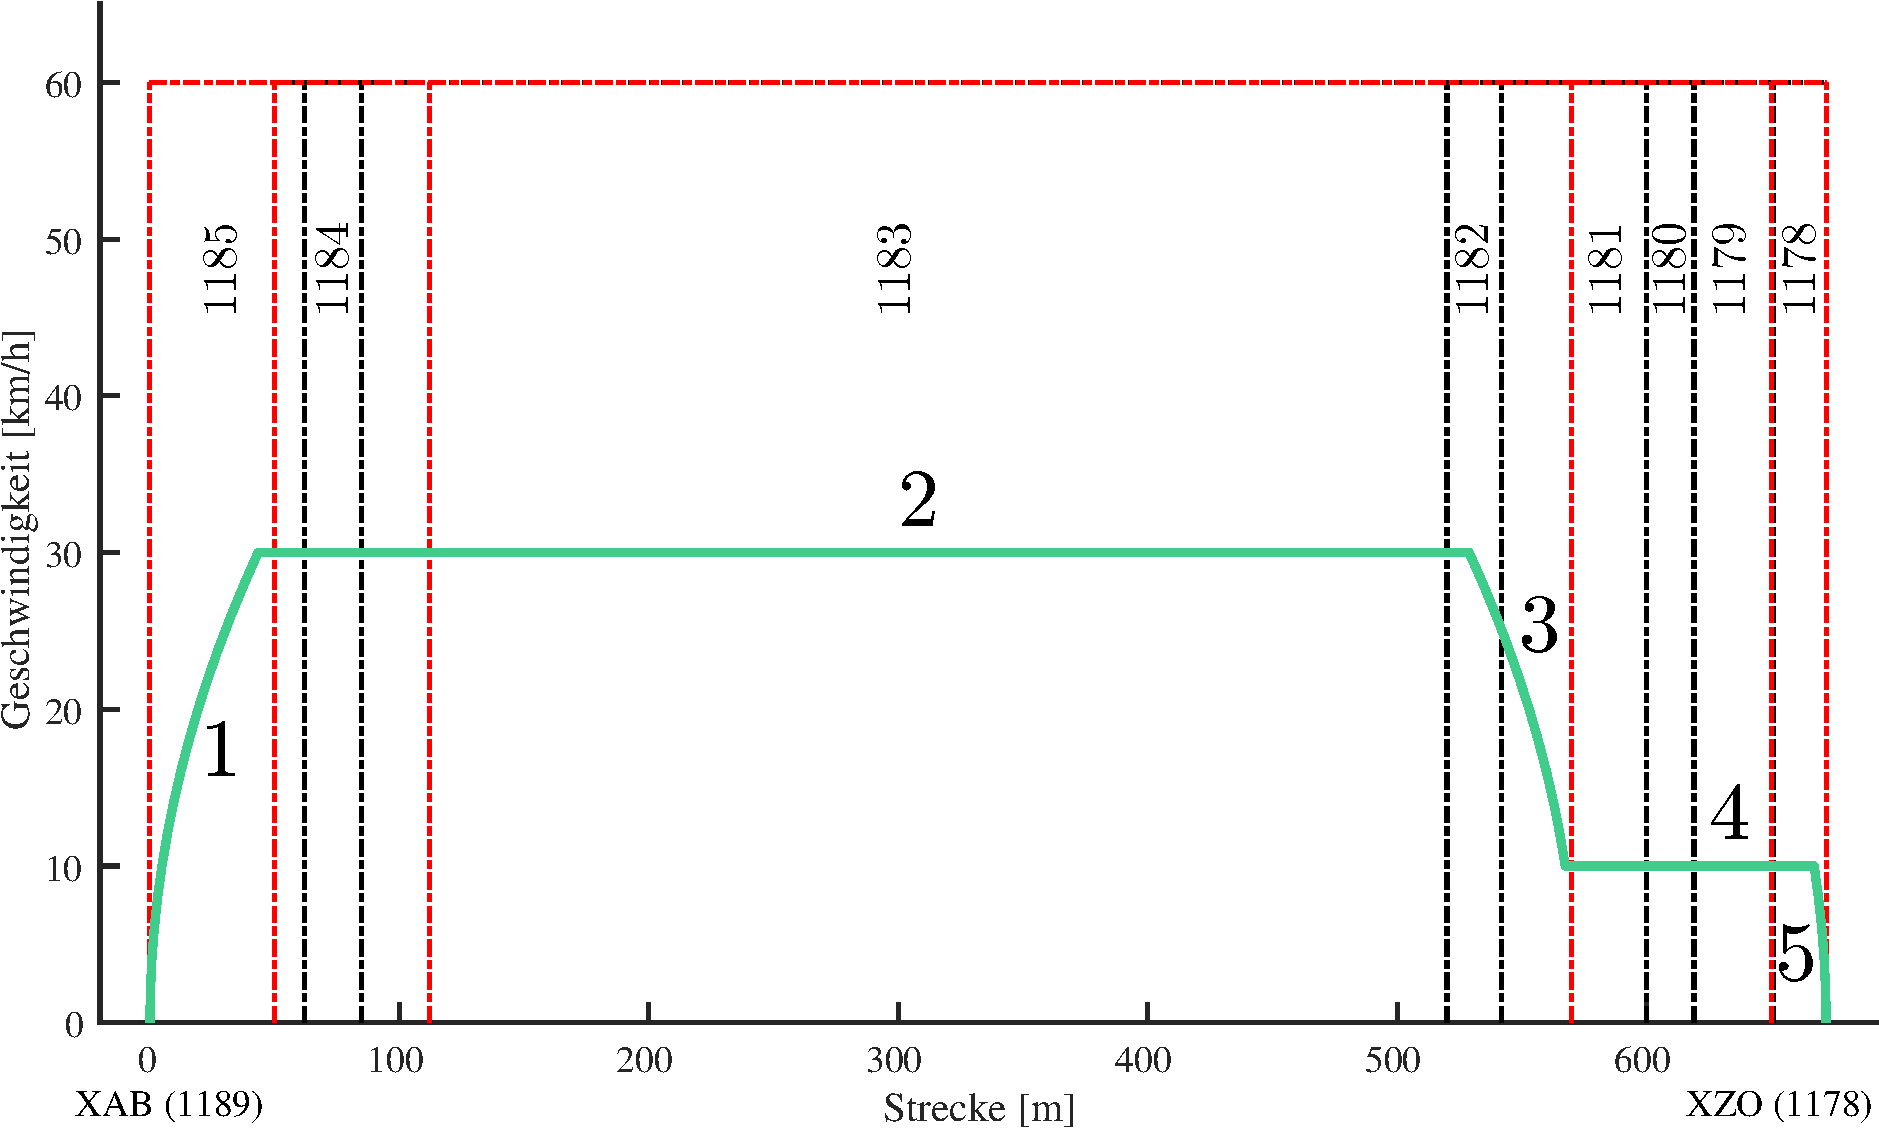
\includegraphics[width=\linewidth]{../images/matlab/it14.pdf}
\caption{\Gls{fahrtverlauf} am Beispiel von der Fahrt von XAB nach XZO}
\label{fig:it14}
\end{figure}
Durch die \textit{\$keyPoints} und die Darstellung des Fahrtverlaufs (Abbildung \ref{fig:it14}) lässt sich der Fahrtverlauf in 5 Abschnitte einteilen. Die Start- und Zielgeschwindigkeit, die Strecke und die Zeit der einzelnen Abschnitte sind in der Tabelle \ref{table:beispielebuef} aufgelistet und werden mittels der Formeln aus Kapitel \ref{formula} überprüft. Bei der Überprüfung werden die Start- und Zielgeschwindigkeiten als Grundlage genommen und untersucht, ob unter Einhaltung der gegebenen Zeit dieselben Werte rauskommen.
\begin{table}
\begin{center}
\begin{threeparttable}
\renewcommand{\arraystretch}{1.2}
\begin{tabular}{c|c|c|c|c|c}
Abschnitt & \makecell{Beschleunigung/\\Verzögerung}& $v_0$ & $v_1$ & Strecke & Zeit\\ \hline
1                   &   ja (Beschleunigung)   & 0 $km/h$ & 30 $km/h$        &         43,40 $m$    & 10,42 $s$   \\ \hline
2                  &       nein& 30 $km/h$ & 30 $km/h$       &    485,43 $m$ & 58,25 $s$   \\ \hline
3                   &       ja (Verzögerung)& 30 $km/h$ & 10 $km/h$           &   38,58 $m$    & 6,94 $s$  \\ \hline
4                   &      nein & 10 $km/h$ & 10 $km/h$       &   99,76 $m$    & 35,92 $s$   \\ \hline
5                   &       ja (Verzögerung)& 10 $km/h$ & 0 $km/h$          &    4,82 $m$  & 3,47 $s$ \\ \hline
$\sum$                   &       ---& --- & ---          &    672 $m$\tnote{1}  & 115 $s$ \\ 
\end{tabular}
\begin{tablenotes}\footnotesize
    \item[1] Die Werte in der Strecken-Spalte sind auf zwei Nachkommastellen gerundet und würden durch das Aufsummieren der Strecken von Abschnitt 1 -- 5 eine Gesamtstrecke von 671,99 $m$ ergeben. Die angegebenen 672 $m$ entsprechen der Summe der Abschnitte\\1 -- 5, ohne dass die einzelnen Strecken gerundet werden.
\end{tablenotes}
\renewcommand{\arraystretch}{1}
\caption{Fahrtverlauf am Beispiel von der Fahrt von XAB nach XZO}
\label{table:beispielebuef}
\end{threeparttable}
\end{center}
\end{table}
\noindent Damit der berechnet Fahrtverlauf den Vorgaben entspricht, muss gelten:
\[t_{ges} = t_1 + t_2 + t_3 + t_4 + t_5 = 115\:s\]
%\[t_{ges} = 115s\]
\[s_{ges} = s_1 + s_2 + s_3 + s_4 + s_5 = 672\:m\]
%\[s_{ges} = 672m\]
Für die Berechnung werden die Strecken und Zeiten in gleichförmige und gleichmäßig beschleunigte Bewegungen unterteilt:
\[t_{ges} = t_{gleichförmige Bewegungen} + t_{gleichmässig Beschleunigte Bewegungen}\]
\[s_{ges} = s_{gleichförmige Bewegungen} + s_{gleichmässig Beschleunigte Bewegungen}\]
\[t_{gleichförmige Bewegungen} = t_2 + t_4\]
\[s_{gleichförmige Bewegungen} = s_2 + s_4\]
\[t_{gleichmässig Beschleunigte Bewegungen} = t_1 + t_3 + t_5\]
\[s_{gleichmässig Beschleunigte Bewegungen} = s_1 + s_3 + s_5\]
Für die gleichmäßig beschleunigten Bewegungen gilt nach den Gleichungen \ref{eq:s_v_ges} und \ref{eq:t_v_ges}:
\[t_1 = \abs{\frac{\frac{30\:km/h}{3,6}-\frac{0\:km/h}{3,6}}{0,8\:m/s^{2}}} = \frac{125}{12}\:s \approx 10,42\:s\]
\[t_3 = \abs{\frac{\frac{10\:km/h}{3,6}-\frac{30\:km/h}{3,6}}{0,8\:m/s^{2}}} = \frac{125}{18}\:s \approx 6,94\:s\]
\[t_5 = \abs{\frac{\frac{0\:km/h}{3,6}-\frac{10\:km/h}{3,6}}{0,8\:m/s^{2}}} = \frac{125}{36}\:s \approx 3,47\:s\]
\[s_1 = \frac{1}{2}\cdot\abs{\frac{{\frac{30\:km/h}{3,6}}^2-{\frac{0\:km/h}{3,6}}^2}{0,8\:m/s^{2}}} = \frac{3125}{72}\:m \approx 43,40\:m\]
\[s_3 = \frac{1}{2}\cdot\abs{\frac{{\frac{10\:km/h}{3,6}}^2-{\frac{30\:km/h}{3,6}}^2}{0,8\:m/s^{2}}} = \frac{3125}{81}\:m \approx 38,58\:m\]
\[s_5 = \frac{1}{2}\cdot\abs{\frac{{\frac{0\:km/h}{3,6}}^2-{\frac{10\:km/h}{3,6}}^2}{0,8\:m/s^{2}}} = \frac{3125}{648}\:m \approx 4,82\:m\]
Dadurch ergibt sich für die Beschleunigungen und Verzögerungen insgesamt eine\linebreak[4]Strecke von:
\[t_{gleichmässig Beschleunigte Bewegungen} = \frac{125}{6}\:s\]
\[s_{gleichmässig Beschleunigte Bewegungen} = \frac{3125}{36}\:m\]
Und für die gleichförmigen Bewegungen gilt dementsprechend:
%\[t_{gleichförmige Bewegungen} = 115s - \frac{125}{6}s\]
\[t_{gleichförmige Bewegungen} = \frac{565}{6}\:s\]
%\[s_{gleichförmige Bewegungen} = 672m - \frac{3125}{36}m\]
\[s_{gleichförmige Bewegungen} = \frac{21067}{36}\:m\]
Für die Berechnung der Strecke und Zeit von der \Gls{beharrungsfahrt} auf 30 $km/h$ gilt nach der Gleichung \ref{eq:t_1_tuning}:
\[t_{2} = \frac{s_{gleichförmige Bewegungen} - \frac{10\:km/h}{3.6} \cdot t_{gleichförmige Bewegungen}}{\frac{30\:km/h}{3.6} - \frac{10\:km/h}{3.6}}\]
\[t_{2} = \frac{\frac{21067}{36}\:m - \frac{10\:km/h}{3.6} \cdot \frac{565}{6}\:s}{\frac{30\:km/h}{3.6} - \frac{10\:km/h}{3.6}}\]
\[t_{2} = \frac{34951}{600}\:s \approx 58,25\:s\]
%\[t_{2} \approx 58,25\:s\]
Daraus folgt nach der Gleichung \ref{eq:s_v_t} für die Abschnitte 2 und 4:
\[t_{4} = \frac{7183}{200}\:s \approx 35,91\:s\]
\[s_{2} = \frac{34951}{600}\:s \cdot \frac{30\:km/h}{3,6}\]
\[s_{2} = \frac{34951}{72}\:m \approx 485,43\:m\]
%\[s_{2} \approx 485,43m\]
\[s_{4} = \frac{7183}{200}\:s \cdot \frac{10\:km/h}{3,6}\]
\[s_{4} = \frac{7183}{72}\:m \approx 99,76\:m\]
%\[s_{4} \approx 99,76m\]
In Summe ergibt das:
\[t_{ges} = \frac{125}{12}\:s + \frac{34951}{600}\:s + \frac{125}{18}\:s + \frac{7183}{200}\:s + \frac{125}{36}\:s = 115\:s\]
%\[t_{ges} = 115s\]
\[s_{ges} = \frac{3125}{72}\:m + \frac{34951}{72}\:m + \frac{3125}{81}\:m + \frac{7183}{72}\:m + \frac{3125}{648}\:m = 672\:m\]
%\[s_{ges} = 672m\]
Wie an den errechneten Werten zu erkennen ist, wurde die Mindestzeit von 20 $s$ auf den \Gls{beharrungsfahrt}en ($t_2$ und $t_4$) eingehalten und die Werte stimmen mit den Werten aus der Tabelle \ref{table:beispielebuef} überein.
\newpage
\section{Visualisierung der Fahrtverläufe} \label{visualisierungFahrtverlaeufe}
Für die Visualisierung der Fahrtverläufe wurde ein MATLAB-Skript geschrieben, welches aus den Arrays \textit{\$cumulativeSectionLengthStart}, \textit{\$cumulativeSectionLengthEnd}, \textit{\$cumulativeSectionLengthStartMod}, \textit{\$cumulativeSectionLengthEndMod}, \textit{\$trainSpeedChange} und \textit{\$trainPositionChange} eines Fahrtverlaufs den kompletten Fahrtverlauf darstellt. Dieses Skript wurde auch verwendet, um die einzelnen Schritte bei der Kalkulation des Fahrtverlaufs in dieser Arbeit darzustellen (wie z. B. in Abbildung \ref{fig:it13}). 

Damit die Daten aus der Berechnung des Fahrtverlaufs von MATLAB eingelesen werden können, wurde die Funktion \textit{safeTrainChangeToJSONFile$($$)$} (Code-Beispiel \ref{lst:safeTrainChangeToJSONFile}) geschrieben, welche die Daten aus den Arrays als JSON-Datei speichert. Für eine bessere Verdeutlichung des Prozesses bei der Ermittlung des Fahrtverlaufs, werden neben dem Ergebnis auch alle vorherigen Iterationsschritte abgebildet.
\begin{lstlisting}[caption={\textit{safeTrainChangeToJSONFile$($$)$}},captionpos=b,label={lst:safeTrainChangeToJSONFile}]
function safeTrainChangeToJSONFile(int $indexCurrentSection, int $indexTargetSection, int $indexCurrentSectionMod, int $indexTargetSectionMod, array $speedOverPositionAllIterations) {
	global $trainPositionChange;
	global $trainSpeedChange;
	global $next_v_max;
	global $cumulativeSectionLengthEnd;
	global $next_v_max_mod;
	global $cumulativeSectionLengthEndMod;

	$speedOverPosition = array_map('toArr', $trainPositionChange, $trainSpeedChange);
	$speedOverPosition = json_encode($speedOverPosition);
	$fp = fopen('../json/speedOverPosition.json', 'w');
	fwrite($fp, $speedOverPosition);
	fclose($fp);

	$v_maxFromUsedSections = array();
	for ($i = $indexCurrentSection; $i <= $indexTargetSection; $i++) {
		array_push($v_maxFromUsedSections, $next_v_max[$i]);
	}
	$VMaxOverCumulativeSections = array_map('toArr', $cumulativeSectionLengthEnd, $v_maxFromUsedSections);
	$VMaxOverPositionsJSon = json_encode($VMaxOverCumulativeSections);
	$fp = fopen('../json/VMaxOverCumulativeSections.json', 'w');
	fwrite($fp, $VMaxOverPositionsJSon);
	fclose($fp);

	$v_maxFromUsedSections = array();
	for ($i = $indexCurrentSectionMod; $i <= $indexTargetSectionMod; $i++) {
		array_push($v_maxFromUsedSections, $next_v_max_mod[$i]);
	}
	$VMaxOverCumulativeSectionsMod = array_map('toArr', $cumulativeSectionLengthEndMod, $v_maxFromUsedSections);
	$VMaxOverPositionsJSon = json_encode($VMaxOverCumulativeSectionsMod);
	$fp = fopen('../json/VMaxOverCumulativeSectionsMod.json', 'w');
	fwrite($fp, $VMaxOverPositionsJSon);
	fclose($fp);

	$jsonReturn = array();
	for ($i = 0; $i < sizeof($speedOverPositionAllIterations); $i++) {
		$iteration = array_map('toArr', $speedOverPositionAllIterations[$i][0], $speedOverPositionAllIterations[$i][1]);
		array_push($jsonReturn, $iteration);
	}
	$speedOverPosition = json_encode($jsonReturn);
	$fp = fopen('../json/speedOverPosition_prevIterations.json', 'w');
	fwrite($fp, $speedOverPosition);
	fclose($fp);
}
\end{lstlisting}
Das MATLAB-Skript ist im Anhang (siehe \ref{anhangMatlab}) dieser Arbeit angehängt und auf weitere Details bezüglich der Funktionsweise wird im Rahmen dieser Arbeit nicht weiter eingegangen.
\newpage
\section{Formeln} \label{formula}
\begin{flushleft}
Für die im folgenden Kapitel verwendeten Einheiten gilt:
\end{flushleft}

\begin{centering}
\begin{conditions}
a     &  Bremsverzoegerung [$m/s^{2}$] \\
v     &  Geschwindigkeit [$m/s$] \\
s     &  Strecke [$m$] \\
t     &  Zeit [$s$]
\end{conditions}
\end{centering}
\subsection{Formeln für gleichmäßig beschleunigte Bewegungen} \label{formulaBeschleunigung}
\noindent Bei einer gleichmäßig beschleunigten Bewegung gilt:\footnote{\citet[S. 22]{richard2011technische}}
\begin{equation}
a(t) = a
\end{equation}
Für die Bestimmung der Geschwindigkeit in Abhängigkeit der Zeit, muss die Beschleunigung $a(t)$ nach der Zeit $t$ integriert werden.\footnote{\citet[S. 20]{richard2011technische}}
\begin{equation}
v(t) = \int a(t) \,dt
\end{equation}
Daraus ergibt sich folgende Gleichung für die Geschwindigkeit in Abhängigkeit der Zeit. Die bei der Integration entstehende Integrationskonstante $v_{0}$ gibt dabei die Startgeschwindigkeit an.
\begin{equation}
v(t) = a \cdot t + v_{0}
\end{equation} %\footnote{ebd. (S. 20)}
Für die Bestimmung der benötigten Zeit muss die Geschwindigkeit erneut integriert werden.\footnote{\citet[S. 20]{richard2011technische}} Die dabei entstehende Integrationskonstante $s_{0}$ gibt die bereits zurückgelegte Strecke an.
\begin{equation}
s(t) = \int v(t) \,dt
\end{equation}
\begin{equation}
s(t) =\frac{1}{2} \cdot a \cdot t^{2} + v_{0}  \cdot t + s_{0}
\end{equation}
Bei der Verwendung dieser Gleichung werden die Integrationskonstanten $v_{0}$ und $s_{0}$ gleich $0$ gesetzt, damit die Gleichungen allgemein gültig sind. Für die Berechnung des Beschleuniguns- und Abbremsverhalten der Fahrzeuge ist es notwendig zu wissen, welche Strecke ein Fahrzeug zurücklegen muss, um von einer Startgeschwindigkeit $v_{0}$ auf eine Zielgeschwindigkeit $v_{1}$ zu beschleunigen bzw. abzubremsen. Dafür wird die Gleichung für die Geschwindigkeit $v(t)$ nach $t(v)$ umgestellt und und in die Gleichung $s(t)$ eingesetzt. Daraus ergibt sich folgende Gleichung für die Strecke in Abhängigkeit von der Geschwindigkeit:
\begin{equation}
t(v) = \frac{v}{a}
\end{equation}
\begin{equation}
s(v) =\frac{1}{2} \cdot \frac{v^{2}}{a}
\end{equation}
Durch die Festlegung von $v_{0} = 0$ wird so die benötigte Strecke ermittelt, welche ein Fahrzeug bei einer gegebenen Bremsverzögerung $a$ benötigt, um von 0 $m/s$ auf eine gegebenen Zielgeschwindigkeit $v_{1}$ zu beschleunigen. Bei der Berechnung des Beschleuniguns- und Abbremsverhalten wird es aber auch zu Situationen kommen, bei denen ein Fahrzeug eine Startgeschwindigkeit hat, für die gilt $v_{0} \neq 0$. Um eine allgemein gültige Gleichung aufzustellen, wird für die Ermittlung der benötigten Strecke bei einer gegebenen Start- und Zielgeschwindigkeit die Strecke berechnet, die das Fahrzeug benötigt, um von 0 $m/s$ auf $v_{1}$ und von 0 $m/s$ auf $v_{0}$ zu beschleunigen. Für die gesuchte Strecke gilt dann: 
\begin{equation}
s(v_{0}, v_{1}) = \abs{s(v_{1}) - s(v_{0})} 
\end{equation}
\begin{equation}
\label{eq:s_v_ges}
s(v_{0}, v_{1}) =\frac{1}{2} \cdot\abs{\frac{v_{1}^{2} - v_{0}^{2}}{a}}
\end{equation}
In der Fahrzeugsteuerung übernimmt diese Berechnung die Funktion \textit{getBrakeDistance()} (Code-Beispiel \ref{lst:getBrakeDistance}). 
\begin{figure}[H]
\begin{lstlisting}[caption={\textit{getBrakeDistance$($$)$} (\textit{functions\_math.php})},captionpos=b,label={lst:getBrakeDistance}]
// Ermittlung der Strecke für eine Beschleunigung bzw. Verzögerung
function getBrakeDistance (float $v_0, float $v_1, float $verzoegerung) {
	return abs(0.5 * ((pow($v_0/3.6,2) - pow($v_1/3.6, 2))/($verzoegerung)));
}
\end{lstlisting}
\end{figure}
\noindent Neben der Berechnung der Strecke ist auch die benötigte Zeit essenziell. Dafür wird mittels $t(v)$ die Zeit berechnet, die das Fahrzeug benötigt, um von 0 $km/h$ auf $v_{0}$ bzw. $v_{1}$ zu beschleunigen und aus der Differenz wird die benötigte Zeit berechnet.
\begin{equation}
\label{eq:t_v_ges}
t(v_{0}, v_{1}) = \abs{\frac{v_{1} - v_{0}}{a}}
\end{equation}
In der Fahrzeugsteuerung übernimmt diese Berechnung die Funktion \textit{getBrakeTime()} (\textit{func\-tions\_""math\-.php}) (Code-Beispiel \ref{lst:getBrakeTime}).
\begin{figure}[H]
\begin{lstlisting}[caption={\textit{getBrakeTime$($$)$} (\textit{functions\_math.php})},captionpos=b,label={lst:getBrakeTime}]
// Ermittelt die Distanz für Brems- und Verzögerungsvorgänge
function getBrakeTime (float $v_0, float $v_1, float $verzoegerung) {
	return abs((($v_1/3.6)/$verzoegerung) - (($v_0/3.6)/$verzoegerung));
}
\end{lstlisting}
\end{figure}
\noindent Für die Berechnung einer Gefahrenbremsung ist es notwendig zu wissen, welche Geschwindigkeit das Fahrzeug an der Position der Gefahrenstelle hat. Dafür wird die Gleichung \eqref{eq:s_v_ges} nach $v_{2}$ umgestellt. Umgesetzt wird diese Gleichung mit der Funktion \textit{get\-Tar\-get\-Brake\-Speed\-With\-Dis\-tance\-And\-Start\-Speed$($$)$} (\textit{func\-tions\_""math\-.php}) (Code-Beispiel \ref{lst:getTargetBrakeSpeedWithDistanceAndStartSpeed}).
\begin{equation}
\label{eq:gefahrenbremsung}
v_{2}(v_{1}, s) = \sqrt{-2 \cdot s \cdot a} + v_{1}
\end{equation}
\begin{figure}[H]
\begin{lstlisting}[caption={\textit{getTargetBrakeSpeedWithDistanceAndStartSpeed$($$)$} (\textit{func\-tions\_""math\-.php})},captionpos=b,label={lst:getTargetBrakeSpeedWithDistanceAndStartSpeed}]
// Ermittelt die Geschwindigkeit, die ein Fahrzeug in einem Bremsvorgang
// nach einer gegebenen Distanz hat.
function getTargetBrakeSpeedWithDistanceAndStartSpeed (float $distance, float $verzoegerung, int $speed) {
	return sqrt((-2 * $verzoegerung * $distance) + (pow(($speed / 3.6), 2)))*3.6;
}
\end{lstlisting}
\end{figure}
\subsection{Formeln für gleichförmige Bewegungen} \label{formulaGleichfoermig}
Bei einer gleichförmigen Bewegung gilt der Grundsatz:\footnote{\citet[S. 22]{richard2011technische}}
\begin{equation}
v(t) = v
\end{equation}
Für die Berechnung der Strecke gilt wie bei der gleichmäßig beschleunigten Bewegung:\footnote{\citet[S. 20]{richard2011technische}}
\begin{equation}
s(t) = \int v(t) \,dt
\end{equation}
\begin{equation}
s(t) =v \cdot t + s_{0}
\end{equation}
Damit die Gleichung allgemeingültig ist, wird die Integrationskonstante $s_{0}$ gleich 0 gesetzt.
\begin{equation}
s(t) =v \cdot t
\label{eq:s_v_t}
\end{equation}
\begin{figure}[H]
\begin{lstlisting}[caption={\textit{distanceWithSpeedToTime$($$)$} (\textit{functions\_math.php})},captionpos=b,label={lst:distanceWithSpeedToTime}]
// Ermittelt die Zeit, die ein Fahrzeug bei einer gegebenen Strecke für
// eine gegebene Distanz benötigt
function distanceWithSpeedToTime (int $v, float $distance) {
	return (($distance)/($v / 3.6));
}
\end{lstlisting}
\end{figure}
\noindent Für die Einhaltung der exakten Ankunftszeit, muss errechnet werden, wie lange das Fahrzeug bei zwei gegebenen Geschwindigkeiten ($v_1$ und $v_2$) auf den jeweiligen Geschwindigkeiten fahren muss, um die Gesamtstrecke ($s_{ges}$) und die Gesamtzeit ($t_{ges}$) einzuhalten. Für die Zeiten und Strecken gilt:
\begin{equation}
\label{eq:t_ges}
t_{ges} = t_{1} + t_{2}
\end{equation}
\begin{equation}
\label{eq:s_ges}
s_{ges} = s_{1} + s_{2}
\end{equation}
Durch das Einsetzen der Gleichung \eqref{eq:s_v_t} in die Gleichung \eqref{eq:s_ges} erhält man folgende Gleichung:
\begin{equation}
\label{eq:s_ges_2}
s_{ges} = v_{1} \cdot t_{1} + v_{2} \cdot t_{2}
\end{equation}
Durch das Umstellen der Gleichung \eqref{eq:t_ges} nach $t_{2}$ und dem Einsetzen in Gleichung \eqref{eq:s_ges_2} gilt für $t_{1}$:
\begin{equation}
\label{eq:t_1_tuning}
t_{1} = \frac{s_{ges} - v_{2} \cdot t_{ges}}{v_{1} - v_{2}}
\end{equation}
\begin{figure}[H]
\begin{lstlisting}[caption={\textit{calculateDistanceforSpeedFineTuning$($$)$} (\textit{functions\_math.php})},captionpos=b,label={lst:calculateDistanceforSpeedFineTuning}]
// Ermittelt die Distanz, um die eine Verzögerung "verschoben" werden müsste,
// damit die exakte Ankunftszeit eingehalten werden kann.
function calculateDistanceforSpeedFineTuning(int $v_0, int $v_1, float $distance, float $time) : float {
	return $distance - (($distance - $time * $v_1 / 3.6)/($v_0 / 3.6 - $v_1 / 3.6)) * ($v_0 / 3.6);
}
\end{lstlisting}
\end{figure}
\newpage
%\addtocontents{toc}{\protect\newpage}
\section{Fazit}
\subsection{Zusammenfassung der Ergebnisse}
Der entwickelte Algorithmus ist in der Lage, für eine gegebene Position und Geschwindigkeit, \acp{infra} inklusive deren Längen und zulässigen Höchstgeschwindigkeiten und einer Zielposition den optimalen \Gls{fahrtverlauf} zu ermitteln, sodass das Fahrzeug ohne eine Überschreitung der zulässigen Höchstgeschwindigkeit und unter Berücksichtigung der Fahrzeuglänge frühestmöglich die Zielposition erreicht. Unter Berücksichtigung der Ankunftszeit wurden Ansätze entwickelt, die dafür sorgen, dass das Fahrzeug -- durch eine Reduzierung der Geschwindigkeit -- pünktlich das Ziel erreicht und durch eine geringere Geschwindigkeit energiesparsamer fährt. Die Ansätze für die Einhaltung der Ankunftszeit ermitteln nicht den optimalsten \Gls{fahrtverlauf}, da in vereinzelten Fällen die Geschwindigkeit reduziert wird, obwohl eine Verschiebung von Brems- bzw. Verzögerungsvorgängen ausreichen würde.

Bei der Entwicklung und Testung der Fahrzeugsteuerung wurden die Fahrten am Rechner auf Grundlage der \textit{MySQL}-Datenbank simuliert. Die dabei ermittelten \Glspl{fahrtverlauf} haben die erforderlichen Bedingungen (Ankunfts-, Abfahrts- und Mindesthaltezeit und zulässige Höchstgeschwindigkeit) eingehalten und die Fahrzeuge haben richtig auf \Glspl{fahrstrasse}-Änderungen reagiert (Einleitung einer Gefahrenbremsung und Berücksichtigung der Signalbegriffe). Bei der Verwendung der Fahrzeugsteuerung im \ac{ebuef} ist es zu Fehlern gekommen, welche in dem folgenden Kapitel \ref{fazit2} erläutert werden.
\subsection{Komplikationen bei dem Betrieb der Fahrzeugsteuerung im \ac{ebuef}} \label{fazit2}
\subsubsection{Einhaltung der Zielposition}
Bei Zugfahrten ist es dazu gekommen, dass die Fahrzeuge den Bremsvorgang zu spät eingeleitet haben und an dem Ausfahrsignal bzw. einem Halt zeigenden Signal vorbei gefahren sind. Für die Fehlerbehebung wurde überprüft, ob die eingetragenen Längen der \ac{infra}e aus der \textit{MySQL}-Datenbank mit den realen Werten des \acp{ebuef} übereinstimmen. Diese mögliche Ursache konnte ausgeschlossen werden und weitere Ursachen konnten nicht ermittelt werden.
\subsubsection{Ermittlung der \Glspl{fahrstrasse}}
Bei der Ermittlung der \Gls{fahrstrasse}n hat die Funktion \textit{getNaechsteAbschnitte$($$)$}$^\ast$ (\textit{functions\_ebuef.php}) in manchen Fällen nicht die eingestellte \Gls{fahrstrasse} und die erwarteten \ac{infra}e wiedergegeben, wodurch für Fahrzeuge kein \Gls{fahrtverlauf} berechnet wurde.
\subsubsection{Kalibrierung der Position}
Bei der Kalibrierung der Fahrzeugposition wurden Positionen ermittelt, welche stark von der realen Position abwichen. Mögliche Ursachen könnten eine falsche Positionsermittlung bei der Berechnung des \Gls{fahrtverlauf}s oder eine nicht rechtzeitige Eintragung der aktuellen Abschnitte in die \textit{MySQL}-Tabelle \textit{fahrzeuge\_abschnitte} sein. Keine der beiden Ursachen konnte eindeutig widerlegt oder belegt werden.
\subsection{Möglichkeiten für eine Weiterentwicklung der Fahrzeugsteuerung}
Durch die kontinuierliche Positionsbestimmung der Fahrzeuge ist es in zukünftigen Weiterentwicklungen der Fahrzeugsteuerung möglich, anstatt der Zugfolge im festen Raumabstand, einen Zugbetrieb im Bremswegabstand (Moving Block) zu realisieren, wodurch die Zugfolgezeiten zweier aufeinander folgender Züge deutlich reduziert werden können.\footnote{\citet[S. 37]{etr}}





















\appendix
\newpage
\bibliography{paper}  % implement the name of the bibtex.bib file
\newpage
%\pagenumbering{Roman} % roman pagenumbers
%\setcounter{page}{8}

\section{Anhang}

\subsection{fahrzeugsteuerung.php} \label{anhangMain}

\lstinputlisting[language=php,nolol]{../php/fahrzeugsteuerung.php}

\newpage

\subsection{functions.php} \label{sortFunctions}

\lstinputlisting[language=php,nolol]{../php/functions/functions.php}

\newpage

\subsection{functions\_fahrtverlauf.php} \label{fahrtverlaufFunctions}

\lstinputlisting[language=php,nolol]{../php/functions/functions_fahrtverlauf.php}

\newpage

\subsection{functions\_math.php} \label{functionsMath}

\lstinputlisting[language=php,nolol]{../php/functions/functions_math.php}

\newpage

\subsection{functions\_cache.php} \label{cacheFunctionsOwn}

\lstinputlisting[language=php,nolol]{../php/functions/functions_cache.php}

\newpage

\subsection{functions\_db.php} \label{functionsDatabase}

\lstinputlisting[language=php,nolol]{../php/functions/functions_db.php}

\newpage

\subsection{global\_variables.php} \label{anhangGlobalVariables}

\lstinputlisting[language=php,nolol]{../php/global_variables.php}

\newpage

\subsection{speed\_over\_position.m} \label{anhangMatlab}

\lstinputlisting[language=matlab,nolol]{../matlab/speed_over_position.m}

\newpage
\newpage
\thispagestyle{empty}
\section*{Eidesstattliche Erklärung}

Ich erkläre hiermit an Eides statt, dass ich die vorliegende Arbeit selbständig und ohne Benutzung anderer als der angegebenen Hilfsmittel angefertigt habe. Die aus fremden Quellen direkt oder indirekt übernommenen Gedanken wurden als solche kenntlich gemacht. Diese Arbeit wurde in gleicher oder ähnlicher Form keiner anderen Prüfungsbehörde vorgelegt und auch noch nicht veröffentlicht.


\vspace{3cm}

\hspace{0.4cm} Berlin, 1. Oktober 2021 \hfill  
\includegraphics[width=115pt]{../images/signature/signature.png} \hspace{1.6cm}



\hspace{1.5cm} Ort, Datum \hfill Unterschrift \hspace{2.1cm}

\end{document}